%!TEX root = main.tex
\chapter{Analyse kohärenter Konstruktionen mit TT-MCTAG}\label{sec-ttmctag}

Eine ausführliche Darstellung des TT-MCTAG-Formalismus wird in Abschnitt~\ref{sec-ttmctag-formalismus} unternommen. Anschlie\ss end werden in Abschnitt~\ref{sec-ttmctag-beispiele} Analysebeispiele für eine Auswahl von Aspekten der kohärenten Konstruktion geliefert. Ein Augenmerk liegt dabei auf dem Vergleich mit HPSG-Modellierungen\is{Head-driven Phrase Structure Grammar (HPSG)}, da hier der Vorteil einer erweiterten Lokalitätsdomäne\is{erweiterte Lokalitätsdomäne} deutlich wird. Dann werde ich in Abschnitt~\ref{sec-ttmctag-grenzen} auf die Grenzen der Ausdrucksstärke von TT-MCTAG eingehen und abschlie\ss end in Abschnitt~\ref{sec-ttmctag-spinal} eine Weiterentwicklung von TT-MCTAG, spinale TT-MCTAG, vorschlagen. 

\section{TT-MCTAG: Der Formalismus}\label{sec-ttmctag-formalismus}\is{TT-MCTAG|(}

TT-MCTAG (SN-MCTAG with Tree Tuples)\footnote{TT-MCTAG wurde zuerst in \cite{Lichte:07} vorgestellt} kombiniert Eigenschaften von SN-MCTAG und V-TAG. Von SN-MCTAG\is{TL-MCTAG with Shared Nodes (SN-MCTAG)} wird die Idee des Node-Sharings\is{Node Sharing} übernommen: Im Fall der \isi{Adjunktion} wird der Zielknoten vom Hilfsbaum nicht vollständig ersetzt, sondern der Wurzelknoten des Hilfsbaums wird in die Lokalitätsdomäne beider Elementarbäume einverleibt. An V-TAG\is{Vector-MCTAG (V-TAG)} erinnert dagegen die valenztheoretische Auf"|fassung von Elementarbaummengen, im Gegensatz zur bewegungsbezogenen Auf"|fassung der Elementarbaummengen in der SN-MCTAG. Dies ist dem Umstand geschuldet, dass TT-MCTAG keiner \isi{Simultanitätsbedingung} unterliegt.

Ein hervorstechender Unterschied zu SN-MCTAG und V-TAG ist sicher auch die Art der Elementarstrukturen in TT-MCTAG. Diese sind nämlich 2-Tupel der Form $\langle \gamma, \{\beta_1,\ldots,\beta_2\}\rangle$, bestehend aus einem lexikalisierten Elementarbaum $\gamma$, dem \textsc{Kopfbaum}\is{Kopfbaum}, und einer Baummenge $\{\beta_1,\ldots,\beta_2\}$, den \textsc{Argumentbäumen}\is{Argumentbaum}. Die derivationelle Bedeutung eines solchen Baumtupels besteht darin, dass die Argumentbäume an den Kopfbaum angeknüpft werden müssen, wobei die Anknüpfungslokalität um das \isi{Node Sharing} erweitert ist. Ein wichtiger Unterschied zur Node-Sharing-Definition bei \cite{Kallmeyer:05} (siehe Abschnitt~\ref{sec-snmctag}), aber auch zur TT-MCTAG-Definition bei \cite{Kallmeyer:09}, ist allerdings, dass die Substitutionsknoten keine geteilten Knoten sein sollen. Im \isi{Ableitungsbaum} muss daher der Kopfbaum den Argumentbaum so dominieren, dass der Pfad ausschlie\ss lich aus Adjunktionen besteht. Mit anderen Worten, Substitutionen\is{Substitution} konstituieren immer Lokalitätsinseln\is{Bewegungsinsel}. All dies erhält eine formalere Explikation in Abschnitt~\ref{sec-ttmctag-definitionen}. Zunächst folgt jedoch ein Beispiel und eine Charakterisierung der Ausdrucksstärke.  

\subsection{Funktionsweise und Ausdrucksstärke} \label{sec-ttmctag-funktionausdruck}

Ein linguistisches Exemplar eines Baumtupels ist in Abbildung \ref{fig-ttmctag-tupel} zu sehen. Entsprechend des valenztheoretischen Verständnisses eines Baumtupels lexikalisiert das valenztragende Verb {\it isst} den \isi{Kopfbaum}, während seine Valenzrollen in den Argumentbäumen\is{Argumentbaum}, d.\,h.\ mittels der dortigen Substitutionsknoten, repräsentiert werden. Die restlichen Formeigenschaften des Kopfbaumes, d.\,h.\ die Struktur der Innenknoten und die Annahme eines leeren Terminals $\epsilon$,  entspricht einem Phrasenstrukturschema, das das System der topologischen Felder\is{topologische Felder} adaptiert. Dazu mehr in Abschnitt~\ref{sec-feldermodell}. Basierend auf dem Baumtupel in Abbildung~\ref{fig-ttmctag-tupel} lassen sich also bei Zuhilfenahme geeigneter Merkmalsstrukturen in den VP-Knoten (siehe ebenfalls Abschnitt~\ref{sec-ttmctag-beispiele}) u.\,a.\ die folgenden V2-Sätze generieren:  

\ex. \label{ex-scrambling}
\a. Peter isst eine Pizza. \label{ex-scrambling-a}
\b. Eine Pizza isst Peter. \label{ex-scrambling-b}
\c. Bei Giovanni isst Peter eine Pizza. \label{ex-scrambling-c}
\d. Bei Giovanni isst eine Pizza Peter. \label{ex-scrambling-d}

\begin{figure}[t]
\centering
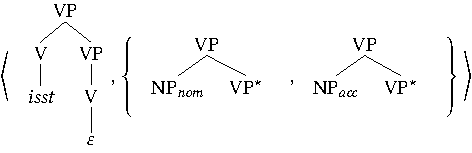
\includegraphics{graphics/abb71.pdf}
\caption{\label{fig-ttmctag-tupel}Baumtupel für das Verb {\it isst}}
\end{figure}

\noindent Die dazugehörigen Ableitungsbäume in Abbildung \ref{fig-ttmctag-ableitung} machen deutlich, warum die Erweiterung der Lokalität mittels Node Sharing notwendig ist. 
\begin{figure}[t]
\begin{center}
\ref{ex-scrambling-a}
\raisebox{-\height}{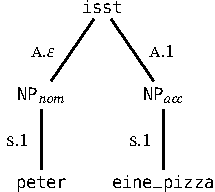
\includegraphics{graphics/abb72a.pdf}}
\hfil
\ref{ex-scrambling-b}
\raisebox{-\height}{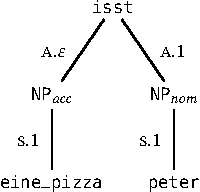
\includegraphics{graphics/abb72b.pdf}}


\vspace{5ex}

\ref{ex-scrambling-c}
\raisebox{-\height}{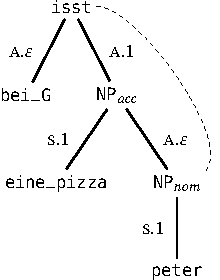
\includegraphics{graphics/abb72c.pdf}}
\hfil
\ref{ex-scrambling-d}
\raisebox{-\height}{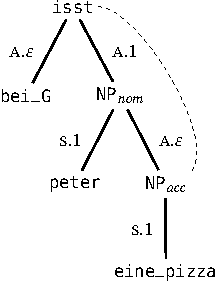
\includegraphics{graphics/abb72d.pdf}}


\end{center}
\caption{\label{fig-ttmctag-ableitung}Ableitungsbäume für die Scramblingdaten in \ref{ex-scrambling}}
\end{figure}
Die Kantenlabel zeigen hier der Übersichtlichkeit halber auch die Art der Verknüpfungsoperation an, also {\sc s}.$p$ für Substitution und {\sc a}.$p$ für Adjunktion an der Adresse $p$. Während die Argumente in \ref{ex-scrambling-a} und \ref{ex-scrambling-b} direkt an den Kopfbaum adjungieren, d.\,h.\ im \isi{Ableitungsbaum} direkt vom Kopfbaum dominiert werden, ist dies in der Ableitung von \ref{ex-scrambling-c} und \ref{ex-scrambling-d} nicht der Fall. Hier ist jeweils eines der Argumente nur indirekt vom Kopfknoten dominiert, angedeutet durch die gestrichelte Linie.\footnote{Um diese indirekte Verknüpfung mit dem Kopfbaum in diesem Fall zu vermeiden, könnte man im Kopfbaum genügend VP-Knoten als Argumentlandeplätze zur Verfügung stellen. So würde die Notwendigkeit des Node Sharings\is{Node Sharing} jedoch nicht gänzlich eliminiert, da weiterhin Modifizierer\is{Angabe} intervenieren können: {\it Bei Giovanni isst heute Peter eine Pizza nach Feierabend.} Hier müssten also noch zusätzliche Landeplätze für Modifizierer angelegt werden. Wir erhielten damit für ein zweistelliges Verb ein dreigliedriges \isi{Mittelfeld}. Diese Multiplizierung der Innenknoten ist mit Rücksicht auf das Ökonomieprinzip\is{Wohlgeformtheitsprinzip!Oekonomieprinzip@Ökonomieprinzip} natürlich fragwürdig. Zudem ist die indirekte Verknüpfung qua Node Sharing bei der Modellierung kohärenter Konstruktionen unvermeidbar.} Dies ist jedoch durch das \isi{Node Sharing} lizenziert, da der \isi{Argumentbaum} über einen Pfad von Wurzeladjunktionen von einem Baum dominiert wird, der wiederum direkt an den \isi{Kopfbaum} adjungiert. Im Ableitungsbaum für \ref{ex-scrambling-c} trifft das zu: {\tt NP$_{nom}$} wird über einen (ein-gliedrigen) Dominanzpfad aus Wurzeladjunktionen von dem Knoten {\tt NP$_{acc}$} dominiert, der eine unmittelbare Tochter des Kopfes {\tt isst} ist. Ebenso im Ableitungsbaum für \ref{ex-scrambling-d}, wo der Kopf {\tt isst} sein Argument {\tt NP$_{acc}$} node-sharing-gerecht dominiert.\is{TT-MCTAG|)}

\is{TT-MCTAG!Ausdrucksstärke|(}
Die \isi{derivationelle Mächtigkeit} von TT-MCTAG reicht aus, um die indizierte Scrambling-Sprache $\mathsf{SCR}^{ind}$\is{indizierte Scramblingsprache ($\mathsf{SCR}^{ind}$)} abzuleiten, z.\,B.\ anhand der Baumtupel in Abbildung~\ref{fig-ttmctag-scr}.  
\begin{figure}[t]
\centering
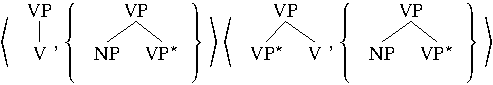
\includegraphics{graphics/abb73.pdf}
\caption{Baumtupel für $\mathsf{SCR}^{ind}$\label{fig-ttmctag-scr}}
\end{figure}
Während der \isi{Verbalkomplex} mit den Kopfbäumen auf der rechten Seite der VP-Projektion gebildet wird, können die NPs mit den Argumentbäumen auf der linken Seite der VP-Projektion in beliebiger Abfolge generiert werden. Es kann dabei immer sichergestellt werden, dass der Argumentbaum an einem vom Kopfbaum geteilten Knoten adjungiert, oder anders ausgedrückt, dass im Ableitungsbaum der Kopfbaum den Argumentbaum node-sharing-gerecht dominiert. Wie  \citet{Sogaard:Lichte:Maier:07} au\ss erdem gezeigt haben, reicht die Ausdrucksstärke von TT-MCTAG  aus, um die \isi{MIX-Sprache} zu generieren.\footnote{In der \isi{MIX-Sprache} über einem Alphabet $A=\{a,b,c\}$ bestehen die Wörter aus einer gleichen Anzahl von $a$'s, $b$'s und $c$'s. Dies ist quasi der Extremfall der freien Wortstellung \citep{Bach:88}.}

Da $\mathsf{SCR}^{ind}$\is{indizierte Scramblingsprache ($\mathsf{SCR}^{ind}$)} jenseits der Ausdrucksstärke von LCFRS\is{Linear Context-Free Rewriting Systems (LCFRS)} liegt und damit TT"=MCTAG womöglich keine MCS-Sprache\is{schwache Kontextsensitivität} ist, stellt sich wie schon bei SN-MCTAG die Frage nach einer Reduzierung der Ausdrucksstärke. Wieder kann man hierfür eine Komplexitätsschranke $k$ bestimmen, die im Fall von TT"=MCTAG die maximale Anzahl von Argumentbäumen angibt, die zu einem Zeitpunkt der Ableitung noch nicht in den abgeleiteten Baum eingefügt wurden, deren Kopfbaum aber schon. $k$ ist also auch die maximale Anzahl der Argumentbäume in einem Baumtupel. Da $k$ beliebig gewählt werden kann, kann auch eine beliebig gro\ss e echte Teilmenge von $\mathsf{SCR}^{ind}$, nämlich $k$-$\mathsf{SCR}^{ind}$, erfasst werden, darunter auch die im Sprachgebrauch vorkommenden Fälle. Diese TT-MCTAG-Variante hei\ss t $k$-TT-MCTAG.

Handelt es sich nun bei TT-MCTAG um einen schwach kontextsensitiven Grammatikformalismus, d.\,h., genügt TT-MCTAG den vier MCS-Kriterien\is{schwache Kontextsensitivität} (siehe S.\,\pageref{ex-kriterien-mcs})? \cite{Kallmeyer:Parmentier:08} zeigen, dass prinzipiell $k$-TT-MCTAG und TAG dieselbe generative Ausdrucksstärke besitzen, indem sie dieselben abgeleiteten Strukturen erzeugen können. Allerdings unterscheiden sie sich hinsichtlich der derivationellen Ausdrucksstärke: TT-MCTAG ist in Bezug auf die Elementarstrukturen flexibler als TAG. Daraus folgt erfreulicherweise, dass TT-MCTAG die Mindestanforderung an seine Ausdrucksstärke erfüllt, indem es wie TAG alle kontextfreien Sprachen und bestimmte kreuzende Abhängigkeiten generieren kann. Was die Verarbeitungskomplexität betrifft, sind die Ergebnisse zwiespältig: Das universelle Erkennungsproblem\is{universelles Erkennungsproblem}\footnote{Die Grammatik ist Teil der Eingabe: Gegeben eine Grammatik $G$ und ein String $s$, ist $s$ in $L(G)$?} für TT-MCTAG ist NP"=vollständig \citep{Sogaard:Lichte:Maier:07}, möglicherweise auch für $k$-TT-MCTAG. Das festgelegte Erkennungsproblem\is{festgelegtes Erkennungsproblem}\footnote{Die Grammatik ist nicht Teil der  Eingabe: Die Grammatik sei immer $G$. Gegeben ein String $s$, ist $s$ in $L(G)$?} kann dagegen für TT-MCTAG (ohne Einschränkung) in polynomieller Zeit gelöst werden \citep{Kallmeyer:Satta:09}. Und letzteres Ergebnis ist das entscheidende in dieser Frage, da wir es, zumindest im Parsingfall, mit einer festgelegten Grammatik zu tun haben. Fehlt noch das Kriterium des konstanten Wachstums\is{konstantes Wachstum} (oder der \isi{Semi-Linearität}). Hierfür liegt noch kein Beweis vor. Zusammenfassend kann man dennoch sagen, dass TT-MCTAG ein ernstzunehmender Kandidat für einen schwach kontextsensitiven Grammatikformalismus darstellt.
\is{TT-MCTAG!Ausdrucksstärke|)}


\subsection{Das Valenzprinzip für TT-MCTAG}\is{Wohlgeformtheitsprinzip!Valenzprinzip für TT-MCTAG|(}

Das Valenzprinzip für TT-MCTAG kann an die Formulierung des Valenzprinzips für TAG in \ref{ex-valenzprinzip-tag} angelehnt werden, muss aber der Auf"|trennung einer Elementarbaumdomäne auf mehrere Teilbäume mit unterschiedlicher Funktion gerecht werden:

\ex. \label{ex-valenzprinzip-mctag}{\bf Valenzprinzip (für TT-MCTAG)} \\ 
Baumtupel entsprechen genau einem Valenzrahmen, wobei gilt:
\a. Der lexikalische Anker im Kopfbaum ist der Valenzträger.
\b. Es besteht ein bijektives Abbildungsverhältnis zwischen Valenzrollen einerseits und Substitutionsknoten in der Elementarbaummenge bzw.\ Substitutionsknoten und Fu\ss knoten im Kopfbaum andererseits.

Die \isi{Fu\ss knoten} der Argumentbäume\is{Argumentbaum} dienen allein der Verknüpfung und haben keinen Valenzbezug. Es liegt in der Natur der Sache, dass eine gewisse Ähnlichkeit zu Rambows CETM für V-TAG\is{Wohlgeformtheitsprinzip!CETM für V-TAG} (vgl.\ \ref{ex-vtag-cetm}, S.\,\pageref{ex-vtag-cetm}) hinsichtlich der Differenzierung der Fu\ss knoten besteht. Nur greift dort  eine Unterscheidung anhand von relativ willkürlich gesetzten Dominanzlinks, während bei TT-MCTAG die Rolle eines Fu\ss knotens aus der Zugehörigkeit zu einem Argumentbaum oder Kopfbaum folgt.   

Zwei weitere wesentliche Unterschiede zu V-TAG\is{Vector-MCTAG (V-TAG)} bestehen darin, dass bei TT-MCTAG Substitutionsknoten immer Lokalitätsinseln\is{Bewegungsinsel} darstellen, was dazu führt, dass maximal eine \isi{Ergänzung} disjunkt sein kann, nämlich die des Fu\ss knotens im \isi{Kopfbaum}. Dagegen ist bei V-TAG eine beliebige Annotation von Lokalitätsinseln mittels Integrity Constraints\is{Integrity Constraint} möglich und daher auch eine beliebige Anzahl disjunkter Ergänzungen per Valenzrahmen.

Kein wesentlicher Unterschied besteht dagegen hinsichtlich der Modellierung der Fakultativität von Valenzrollen\is{Ergänzung!fakultative}. Die kann sowohl bei TT-MCTAG als auch bei V-TAG durch lexikalische Ambiguität erreicht werden, indem es im Lexikon z.\,B.\ zwei Einträge (d.\,h.\ Baumtupel bzw.\ Baummengen) für {\it isst} gibt -- einen mit Akkusativobjekt, einen ohne. Dank der tupelartigen Globalstruktur ist es jedoch leicht denkbar, anders als bei TAG und den angesprochenen Varianten, diese Baumtupel-Alternativen mittels einer simplen Erweiterung der Baumtupelstruktur zu vereinigen: Die obligatorischen und fakultativen Valenzrollen können nämlich in unterschiedlichen Argumentmengen repräsentiert werden. Ein solches 3-stelliges Baumtupel für {\it isst} mit zwei Argumentmengen ist in Abbildung \ref{fig-ttmctag-3tupel} dargestellt. 
\begin{figure}[t]
\centering
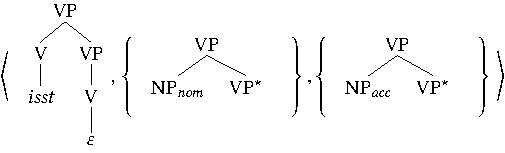
\includegraphics{graphics/abb74.pdf}
\caption{\label{fig-ttmctag-3tupel}3-stelliges Baumtupel für das Verb {\it isst} mit getrennten Argumentmengen für obligatorische und fakultative Ergänzungen}
\end{figure} 
Die obligatorischen Argumente befinden sich hier in der ersten Argumentmenge und die fakultativen Argumente in der zweiten. Im Weiteren werde ich jedoch auf diese Faktorisierung verzichten und durchgehend zweistellige Baumtupel verwenden.
\is{Wohlgeformtheitsprinzip!Valenzprinzip für TT-MCTAG|)}   


\subsection{Definitionen}\label{sec-ttmctag-definitionen}\is{TT-MCTAG!Definition|(}

Die folgenden Definitionen orientieren sich an denen in \cite{Kallmeyer:05} und \cite{Kallmeyer:09}, wobei die dortigen Definitionen bedingt durch unterschiedliche Zielsetzungen nicht vollständig kongruent sind. Der Zwischenweg, den ich hier gehe, versucht von beiden Ansätzen zu einer möglichst passgenauen, dem Verständnis förderlichen Definitionsvariante zu gelangen. 

Die Definition von TAG\is{Tree Adjoining Grammar (TAG)}, d.\,h.\ der Elementarstrukturen ohne Operationen, kennt keine gro\ss e Variationsbreite und kann direkt aus \cite{Kallmeyer:09} übernommen werden:   
\begin{definition}[Tree Adjoining Grammar]
Eine {\it Tree Adjoining Grammar} (TAG) ist ein Tupel $G = \langle N,T,S,I,A,f_{\mathit{OA}},f_{\mathit{SA}} \rangle$, wobei gilt:
\begin{itemize}
  \item $N,T$ sind disjunkte Alphabete nicht-terminaler und terminaler Symbole.
  \item $S \in N$ ist das Startsymbol.
  \item $I$ ist die endliche Menge der Initialbäume und $A$ ist die endliche Menge der Hilfsbäume.
  \item $f_{\mathit{OA}}$: $\{ v | v$ ist ein Knoten eines Elementarbaums $\gamma \in I \cup A \} \to \{0,1\}$, \\
        $f_{\mathit{SA}}$: $\{ v | v$ ist ein Knoten eines Elementarbaums $\gamma \in I \cup A \} \to P(A)$ ,\\
        wobei $P(A)$ die Potenzmenge von $a$ ist und für jedes Blatt $v$ gilt: $f_{\mathit{OA}}(v) = 0$ und $f_{\mathit{SA}}(v) = \emptyset$. 
\end{itemize}
\end{definition}
Eine TAG wird oft als 5-Tupel notiert, indem die Adjunktionsbeschränkungen\is{Adjunktionsbeschränkung} weggelassen werden. Die Adjunktionsbeschränkungen sind hier enthalten, da sie die NA-Beschränkung\is{Adjunktionsbeschränkung} auf den Blättern explizit machen, die in weiten Teilen der TAG-Literatur stillschweigend angenommen wird. Eine Definition der \isi{Substitution} und \isi{Adjunktion} überspringe ich hier und verweise auf \citet[59f]{Kallmeyer:09}.

Eine TAG-Ableitung wird gemeinhin als \isi{Ableitungsbaum}, d.\,h.\ als baumförmiger Ableitungsgraph, repräsentiert. Die folgende Definition des TAG"=Ableitungsbaums legt fest, wie die Repräsentation einer vollständige TAG-Ableitung als Ableitungsbaum bestimmt ist (siehe \citealt[196]{Kallmeyer:05}):   
\begin{definition}[TAG-Ableitungsbaum]
Sei $G = \langle N,T,S,I,A,f_{\mathit{OA}},f_{\mathit{SA}} \rangle$ eine TAG und $D = \langle V,E \rangle$ ein Baum mit Knoten $V$ und gelabelten Kanten $E \subset V \times V \times \mathbb{N}^*$. $D$ ist ein TAG-Ableitungsbaum, falls gilt:
\begin{itemize}
  \item $V$ ist eine Menge von Instanzen von Elementarbäumen aus $I \cup A$.
  \item Für jede Kante $\langle \gamma_1, \gamma_2 , p\rangle \in E$ gilt:
  \begin{itemize}
    \item Entweder $\gamma_2$ ist ein Initialbaum, dann ist $p$ die Gorn-Adresse eines nicht"=terminalen Blattes in $\gamma_1$, das $\gamma_2$ substituiert;
    \item oder $\gamma_2$ ist ein Hilfsbaum, dann ist $p$ die Gorn-Adresse eines nicht"=terminalen Innenknotens in $\gamma_1$, an den $\gamma_2$ adjungiert;  
  \end{itemize}
  \item Für jedes nicht-terminale Blatt $n$ mit Gorn-Adresse $p_n$ in einer Elementarbauminstanz $\gamma_n \in V$ gilt:
  \begin{itemize}
    \item Entweder $n$ ist kein Fu\ss knoten, dann gibt es genau eine Kante $\langle \gamma_n , \gamma,$ $p_n \rangle \in E$ mit $\gamma \in V$;
    \item oder $n$ ist ein Fu\ss knoten, dann gibt es genau eine Kante $\langle \gamma , \gamma_n, p \rangle \in E$ mit $\gamma \in V$ und $p \in \mathbb{N}^*$.   
  \end{itemize}
  \item Für jeden Innenknoten $n$ einer Elementarbauminstanz $\gamma_n \in V$ mit Gorn-Adresse $p_n$ und OA-Adjunktionsbeschränkung gilt: Es gibt genau eine Kante $\langle \gamma_n , \gamma, p_n \rangle \in E$ mit $\gamma \in V$.
\end{itemize}
\end{definition}
Eine Elementarbauminstanz eines Elementarbaums $\gamma$ aus der Grammatik $G$ ist ein konkretes Objekt mit genau den Eigenschaften von $\gamma$. Analog verhält es sich bei Baummengeninstanzen.\footnote{Ein Einwand könnte lauten, dass hier durch den Einsatz von Elementarbauminstanzen die Menge der Ableitungsbäume\is{Ableitungsbaum} für einen gegebenen abgeleiteten Baum\is{abgeleiteter Baum} unendlich sei, da auch die Menge der Instanzen einer Elementarbaumklasse unendlich ist. Das ist jedoch beabsichtigt und kein Nachteil. Ein bijektives Verhältnis zwischen Ableitungsbaum und dem abgeleiteten Baum kann nur bezogen auf die Grammatik gefordert werden, d.\,h.\ wenn die Elementarbauminstanzen wieder auf Elementarbäume der Grammatik abgebildet werden. Der Ableitungsbaum repräsentiert hier also einen einzelnen, konkreten Parse.}

Bei der Definition von MCTAG\is{Multi-Component TAG (MCTAG)} werden der Definition von TAG Baummengen hinzugefügt:
\begin{definition}[MCTAG]
Eine Multi-Komponenten TAG (MCTAG) ist ein Tupel \linebreak $G = \langle N,T,S,$ $I,A,\mathcal{A} \rangle$, wobei $G_{TAG} = \langle N,T,S,I,A\rangle$ eine TAG und $\mathcal{A}$ eine Teilmenge der Potenzmenge von $I \cup A$ ist.
\end{definition}
Dies deckt sich ebenfalls mit der MCTAG-Definition in \cite{Kallmeyer:05}. Dagegen definiert \cite{Kallmeyer:09} $\mathcal{A}$ als die Partition von $I \cup A$. Eine Partition $\mathcal{P}$ einer Menge $M$ schlie\ss t jedoch aus, dass ein  $\gamma \in M$ ein Element in zwei oder mehr Mengen aus $\mathcal{P}$ ist. In der Menge $I \cup A$ befinden sich deshalb Elementarbäume identischer Form, quasi Instanziierungen einer Elementarbaum-Superklasse, die jeweils genau einer Elementarbaummenge zugeordnet werden. Die Zugehörigkeit eines Elementarbaums zu mehreren Baummengen in der Grammatik erscheint unter diesen Voraussetzungen als Täuschung. Für unsere Zwecke ist diese zweifache Instanziierung, sowohl innerhalb der Grammatik als auch beim Parsen, nicht notwendig, denn für eine eindeutige Zuordnung der Elementarbäume zu den Baummengen im Ableitungsbaum reicht die Parsing-Instanziierung aus. Es bieten sich dann die folgenden Definitionsansätze für $\mathcal{A}$ an: Entweder $\mathcal{A}$ ist eine Teilmenge der Potenzmenge von $I \cup A$, wobei dann ein Elementarbaum der Grammatik zwar in mehreren Baummengen auf"|treten kann, aber nicht in einer Baummenge mehr als einmal. Oder $\mathcal{A}$ ist eine Menge von Baumlisten oder Baumsequenzen wie bei \cite{Weir:88}, wodurch keine Einschränkung dieser Art besteht. Ob man die Baumlisten schlie\ss lich "`Baummengen"' nennt, kann als die Folge einer terminologische Konventionalisierung betrachtet werden. In meinen Augen reicht jedoch erstere Definitionsalternative bei der Grammatikimplementierung aus.

Die Einschränkungen bei der Verwendung von Elementarbaummengen können deklarativ über Einschränkungen auf den MCTAG-Ableitungsbäumen\is{Ableitungsbaum} festgehalten werden:  
\begin{definition}[MCTAG-Ableitungsbaum]
Sei $G = \langle N,T,S,I,A,\mathcal{A} \rangle$ eine MCTAG mit einer TAG $G_{TAG} = \langle N,T,S,I,A\rangle$ und sei $D = \langle V,E \rangle$ ein  TAG-Ableitungsbaum. $D$ ist ein MCTAG-Ableitungsbaum gdw.:
\begin{itemize}
  \item Für jedes $v \in V$ gibt es genau eine Baummengeninstanz $\Gamma$ einer Baummenge $\Gamma^e \in \mathcal{A}$, so dass $v \in \Gamma$.
  \item (MC) Wenn $\Gamma$ eine Baummengeninstanz einer Baummenge $\Gamma^e \in \mathcal{A}$ ist und es gibt ein $v \in V$, so dass $v \in \Gamma$, dann gilt für jedes $\gamma \in \Gamma$, $\gamma \in V$.
\end{itemize}
\end{definition}
Die erste Einschränkung bewirkt, dass die benutzen Elementarbäume tatsächlich immer aus Baummengeninstanzen stammen. Die zweite Einschränkung, die sogenannte MC-Einschrän\-kung (\citealt[197]{Kallmeyer:05}; \citealt[64]{Kallmeyer:09}), fordert andererseits, dass alle Elementarbäume aus Baummengeninstanzen verwendet werden müssen. Diese beiden Einschränkungen sind allen MCTAG"=Varianten eigen. Abhängig von der MCTAG-Variante kommen noch weitere Einschränkungen hinzu, wie etwa bei NL-MCTAG die \isi{Simultanitätsbedingung} (siehe \citealt[66]{Kallmeyer:09}). Zu den spezifischen Einschränkungen für TT-MCTAG-Ableitungs\-bäume, die bisher unter dem Begriff des Node Sharings\is{Node Sharing} angesprochen wurden, kommen wir gleich. Zunächst jedoch folgt die Definition der TT"=MCTAG"=Elementarstrukturen. Diese werden, ähnlich wie bei \citet[71]{Kallmeyer:09}, als MCTAG"=Baummengen definiert, in denen mittels der Kopfabbildung $h$ ein Elementarbaum als \isi{Kopfbaum} festgelegt wird:\footnote{\citet[71]{Kallmeyer:09} legt den Kopfbaum als denjenigen Elementarbaum fest, der lexikalisiert ist. Da ich nicht ausschlie\ss en möchte, dass mehr als ein Elementarbaum eines Baumtupels lexikalisiert ist oder dass der Kopfbaum keinen lexikalischen Anker (oder nur ein leeres Wort als Anker) besitzt, gebe ich hier eine etwas allgemeinere Definition.}
\begin{definition}[TT-MCTAG]
Sei $G = \langle N,T,S,I,A,\mathcal{A} \rangle$ eine MCTAG und $h: \mathcal{A} \to I\cup A$ eine Kopfabbildung, dann ist $G'= \langle N,T,S,I,A,\mathcal{A},h \rangle$ eine Baumtupel-MCTAG mit Node Sharing (TT-MCTAG). 
\end{definition}
Jedes Baumtupel $\Gamma$ hat also eigentlich die Form $\{ \gamma, \beta_1,\ldots,$ $\beta_n\}$ mit $h(\Gamma) = \gamma$. $\gamma$ ist der Kopfbaum und $\beta_1 \ldots \beta_n$ sind die Argumentbäume. Wir notieren solch eine Baummenge aber weiterhin als 2-Tupel $\langle \gamma, \{\beta_1, \ldots, \beta_n\} \rangle$. Für eine Verkürzung der Schreibweise sagen wir außerdem: Die Menge der Argumentbäume in einer Baummenge $\Gamma$ ist $arg(\Gamma)$. Ein TT-MCTAG-Ableitungsbaum\is{Ableitungsbaum} kann dann folgenderma\ss en definiert werden:
\begin{definition}[TT-MCTAG-Ableitungsbaum]\label{def-ttmctag-ab}
Sei $G = \langle N,T,S,I,A,\mathcal{A},h \rangle$ eine TT-MC\-TAG und sei $D = \langle V,E \rangle$ ein MCTAG-Ableitungsbaum. $D$ ist ein TT-MCTAG-Ablei\-tungs\-baum gdw.:
Für jedes $v \in V$, wobei $v \in arg(\Gamma)$ mit einer Baummengeninstanz $\Gamma$, gilt:
\begin{itemize} 
  \item $\langle h(\Gamma),v,p \rangle \in E$ für beliebiges $p$, oder
  \item es gibt Instanzen von Hilfsbäumen $u_1, \ldots, u_n \in V$ mit $n>1$ , so dass
  \begin{itemize}
    \item $\langle h(\Gamma),u_1,p \rangle \in E$ für beliebiges $p$, und
    \item $\langle u_i,u_{i+1},\epsilon \rangle \in E$ für $1 \leq i < n$, und
    \item $\langle u_n,v,\epsilon \rangle \in E$.
  \end{itemize}
\end{itemize}  
\end{definition}
Die spezifischen Einschränkungen für TT-MCTAG-Ableitungbäume enthalten die Bedingungen des Node Sharings\is{Node Sharing}, die wir bereits informell kennengelernt haben, d.\,h.\ ein Argumentbaum ist entweder unmittelbare Tochter des Kopfbaums, oder der Kopfbaum dominiert seinen Argumentbaum Node-Sharing-gerecht. In Definition~\ref{def-ttmctag-ab} manifestiert sich zudem ein wichtiger, ebenfalls bereits angesprochener Unterschied zu SN-MCTAG\is{TL-MCTAG with Shared Nodes (SN-MCTAG)} \citep{Kallmeyer:05,Kallmeyer:09} bezüglich der Reichweite des Node-Sharings: Anders als bei SN-MCTAG werden bei TT-MCTAG die Substitutionsknoten nicht geteilt.\footnote{Die formalen Eigenschaften ändern sich dadurch jedoch nicht (Kallmeyer, persönliche Mitteilung 2011).} Die Dominanzpfade zwischen Kopfbaum und Argumentbaum sind also nur dann Node-Sharing-gerecht, wenn sie ausschlie\ss lich aus Adjunktionen am Wurzelknoten bestehen.
Man beachte schlie\ss lich, dass unter den spezifischen Einschränkungen für TT-MCTAG die \isi{Simultanitätsbedingung} fehlt, und dass daher die Baumtupel-Elemente nicht-simultan verwendet werden können.

Um die schwache Äquivalenz mit LCFRS\is{Linear Context-Free Rewriting Systems (LCFRS)} und damit eine Kompatibilität mit MCS zu erreichen, wird dem TT-MCTAG-Ableitungsbaum\is{Ableitungsbaum} eine weitere Ein"-schränkung auferlegt:
\begin{definition}[$k$-TT-MCTAG] Ein TT-MCTAG-Ableitungsbaum $D = \langle V,E \rangle$ hat den Rang $k$, falls es kein $v \in V$ gibt, so dass
\begin{itemize}
  \item[] $|\{ v'| $ 
  \begin{itemize}
  \item[]$\langle v,v',p\rangle \in E^+ $ und 
  \item[]$v' \in arg(\Gamma)$ und 
  \item[]$ \langle v,h(\Gamma)\rangle \not\in E^*$ 
  \end{itemize} 
  \item[]$\}|  > k$  
\end{itemize}
\end{definition}
$E^+$ ist die transitive Hülle und $E^*$ die reflexiv-transitive Hülle von $E$, wobei von der Gorn-Adresse abgesehen wird.
Die Begrenzung der Anzahl noch unverknüpfter Argumentbäume (bereits verknüpfter Kopfbäume) in jedem Ableitungsschritt durch eine Komplexitätschranke $k$ entspricht in Form und Funktion dem $k$ aus SN-MCTAG[$k$] (siehe Abschnitt~\ref{sec-snmctag}).  
\is{TT-MCTAG!Definition|)}

\section{Analysebeispiele} \label{sec-ttmctag-beispiele}

In diesem Abschnitt werden beispielhaft TT-MCTAG-Analysen von Kohärenz"-phänomenen des Deutschen vorgeführt. Abdeckungslücken prinzipieller Art werden separat in Abschnitt~\ref{sec-ttmctag-grenzen} behandelt. 

\subsection{Die Integration des topologischen Feldermodells}\label{sec-feldermodell}\is{topologische Felder|(}

Das topologische Feldermodell vereint grundlegende Abfolgeregeln des deutschen Satzbaus in einem linear geordneten Schema sogenannter \textsc{Felder}.\footnote{Siehe \cite{Reis:80}, \cite{Askedal:86} und \cite{Hoehle:86} für eine umfassendere Darstellung und weitere Literaturangaben.} Die Benennung und Definition der Felder erfolgt zwar nicht immer ganz einheitlich (gerade bei älteren Arbeiten), aber es hat sich seit den 1980ern ein gewisser Konsens herausgebildet.\footnote{Vgl.\ aber die Bemerkung von \citet[286]{Sternefeld:06}, dass man sich auf keine "`Standardversion"' berufen könne. Warum das so sei, erklärt er leider nicht.} Ich halte mich im Folgenden an das  Feldermodell in Tabelle~\ref{ex-feldermodell}, das u.\,a.\ der Darstellung in \citet[216ff]{Askedal:86} recht nahe kommt. 

\begin{table}[t]
\centering
\begin{tabular}{c|c|c|c|cc}
{\bf Vorfeld} & {\bf LK} & {\bf Mittelfeld} & {\bf RK} & {\bf Nachfeld} \\
\cline{1-5}
\multicolumn{3}{c|}{Restfeld} & Schlussfeld \\
\cline{1-5}
\cline{1-5}
{\it Marlene} & {\it isst} & {\it heute Plätzchen} & & {\it obwohl \ldots} & (V2) \\
{\it Heute} & {\it hat} & {\it Marlene} & {\it durchgeschlafen} & {\it obwohl \ldots} & (V2) \\
& {\it hat} & {\it Marlene} {\it heute} & {\it durchgeschlafen} & & (V1) \\
 & {\it dass} & {\it Marlene} {\it heute} & {\it durchgeschlafen} {\it hat} & & (VE)
\end{tabular}
\caption{\label{ex-feldermodell}Topologisches Feldermodell und Satztypen}
\end{table}

Dreh- und Angelpunkt des Feldermodells ist die Unterscheidung zwischen den Verben, deren Verbalfelder\is{Verbalfeld} ein \isi{Kohärenzfeld} bilden, und allen anderen unmittelbaren Konstituenten des Satzes, d.\,h.\ Nominalphrasen, Adjektive, Gliedsätze, etc. Die linke \isi{Satzklammer} (LK) und die rechte Satzklammer (RK) werden von den Verben besetzt, während die restlichen Satzglieder über \isi{Vorfeld}, \isi{Mittelfeld} und \isi{Nachfeld} verteilt sind. Wie in Tabelle~\ref{ex-feldermodell} angezeigt, entspricht das Vorfeld, die linke Satzklammer und das Mittelfeld in der Bechschen Terminologie dem \isi{Restfeld} und die rechte Satzklammer dem \isi{Schlussfeld}.\footnote{Zur Bechschen Terminologie siehe Abschnitt \ref{sec-kohaerenz-einf}.} Darüber hinaus gelten \textsc{feldspezifische Besetzungsregeln}: (i) Das Vorfeld wird von maximal einem \isi{Satzglied} besetzt; (ii) die linke Satzklammer enthält nur das finite Verb (exklusive abtrennbaren Verbzusatz) oder einen \isi{Komplementierer}; (iii) die rechte Satzklammer kann finite und infinite Verben enthalten; (iv) das Nachfeld enthält meist Präpositionalphrasen, Nebensätze und Infinitivphrasen, aber auch Adverbial- und Nominalphrasen \citep[Kapitel~13]{Mueller:99}.

Abhängig von der Position des finiten Verbs werden die Satztypen\is{Satz} V1, V2 und VE unterschieden. Steht das finite Verb satzinitial, ist also das Vorfeld leer, dann liegt V1\is{Satz!V1-} (oder Verberst-Stellung) vor. Ist das Vorfeld besetzt und steht das finite Verb weiterhin in der linken Satzklammer, dann liegt V2\is{Satz!V2-} (oder Verbzweit-Stellung) vor. Während V1 und V2 nur in der Besetzung des Vorfelds voneinander abweichen und das Stellungspezifikum sogennanter Haupsätze darstellen, ist der Satztyp VE\is{Satz!VE-} (mit Verbend- oder Verbletzt-Stellung) bei sogenannten Nebensätzen anzutreffen. Das finite Verb steht hier im Schlussfeld, potentiell flankiert von infiniten Verben, während das Vorfeld leer bleibt und in der linken Satzklammer nur Komplementierer stehen können.\footnote{\cite{Hoehle:86} sieht jeweils eigene Positionen für Komplementierer und vorangestellte finite Verben vor ("`C"' und "`FINIT"'), doch eine Reihe empirischer Belege spricht für eine Besetzung desselben Feldes (siehe \citealt[Section~2]{Kathol:01}).} 

Das lineare Felderschema kann auf unterschiedlichste Weise in einer hierarchischen \isi{Phrasenstruktur} ausgedrückt werden. Bei den folgenden Analysen werde ich mich weitgehend an das rechtsverzweigende Phrasenstrukturschema\is{Phrasenstruktur!rechtsverzweigende} in Abbildung~\ref{fig-ttmctag-ps-1} halten.\footnote{Bei Analysen der partiellen Voranstellung\is{Voranstellung!partielle} verwende ich aus Ökonomiegründen eine ternäre Struktur unterhalb des Vorfeldknotens. Siehe z.\,B.\ Abbildung~\ref{fig-ttmctag-front}, S.\,\pageref{fig-ttmctag-front}.}
\begin{figure}[t]
\centering
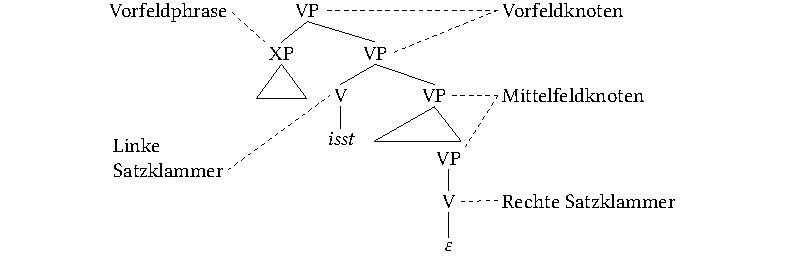
\includegraphics{graphics/abb75.pdf}
\caption{\label{fig-ttmctag-ps-1} Phrasenstrukturschema eines V2-Satzes}
\end{figure} 
Wie durch gestrichelte Linien angedeutet entsprechen darin unterschiedliche Felder (abgesehen vom Nachfeld) unterschiedlichen nicht-termi\-nalen Knoten der Phrasenstruktur. Die Vorfeldknoten\is{Vorfeld} dominieren also den Knoten der linken Satzklammer\is{Satzklammer} und die Mittelfeldknoten\is{Mittelfeld}, und letztere wiederum den Knoten der rechten Satzklammer. Diese rechtsverzweigende Gestalt der Phrasenstruktur\is{Phrasenstruktur!rechtsverzweigende} ist in Syntaxmodellen weit verbreitet und wird u.\,a.\ durch transformationsgrammatische Überlegungen\footnote{Überaus wirkungsmächtig  ist z.\,B.\ die Vorstellung, dass das Verb in der rechten Satzklammer basisgeneriert wird und dann im Zuge von Transformationsprozessen aus dieser Basisposition in die linke Satzklammer bewegt wird (siehe \citealt[Abschnitt~2.2.2]{Stechow:Sternefeld:88}; \citealt[Abschnitte~III.4 und III.5]{Sternefeld:06}; \citealt[Abschnitt~3.2]{Mueller:10}). Bewegungstransformationen\is{Bewegung} zielen dabei auf eine "`höhere"' Position im Syntaxbaum ab.} und Überlegungen zur Syntax-Semantik-Schnittstelle\footnote{Eine der Kernannahmen ist die Korrelation von \isi{c-Kommando} und \isi{Skopus}. Daraus und aus der Annahme, dass im \isi{Mittelfeld} (in der Basisposition) eine Konstituente Skopus über nachfolgende Konstituenten nimmt (und nicht anders herum), ist der rechtsverzweigende Charakter des Mittelfelds notwendig gegeben.% Man beachte, dass zwar in bisherigen Vorschlägen zur Syntax-Semantik-Schnittstelle bei LTAG (\citealt{Gardent:Kallmeyer:03, Kallmeyer:Romero:08}) nicht der abgeleiteten Baum sondern der Ableitungsbaum Grundlage der semantischen Komposition ist, dass aber auch dort die Skopusfestlegung anhand der Reihenfolge auf der verbalen Projektionslinie im abgeleiteten Baum erfolgt.
} motiviert.

Eine wichtige Einschränkung dieser Phrasenstrukturen\is{Phrasenstruktur} wird im Folgenden als \textsc{Vorfeldbündelung}\is{Vorfeldbündelung} bezeichnet: Das Vorfeld nimmt nicht mehr als eine Projektionsstufe der VP ein, d.\,h.\ es gibt maximal eine Vorfeldphrase. Diese Einschränkung entspricht der  Besetzungsregel für Vorfelder (siehe Tabelle~\ref{ex-feldermodell}), nämlich dass das Vorfeld von maximal einem Satzglied besetzt wird. Es stellt sich allerdings die Frage, ob diese Besetzungsregel nicht zu restriktiv und tatsächlich unter bestimmten Umständen eine \isi{mehrfache Vorfeldbesetzung} möglich ist. Eine mehrfache Vorfeldbesetzung scheint es etwa in \ref{ex-vorfeld-mehrfach} zu geben:

\ex.  [Alle Träume] [gleichzeitig] lassen sich nur selten verwirklichen.\\
\citep[(3b)]{Mueller:05b}\label{ex-vorfeld-mehrfach}

Ich schließe mich der Einschätzung von \cite{Mueller:03,Mueller:05b} an, dass auch in Fällen wie \ref{ex-vorfeld-mehrfach} eine Vorfeldbündelung (bestehend aus einer VP mit leerem Kopf) angenommen werden sollte.
\is{topologische Felder|)}


%\subsubsection*{Implementierung}

Die abgeleiteten Bäume der hier vorgestellten TT-MCTAG-Implementierung sollen Instanzen des Phrasenstrukturschemas in Abbildung \ref{fig-ttmctag-ps-1} sein, so weit es V2-Sätze\is{Satz!V2-} betrifft. Die TT-MCTAG-Implementierung unterliegt also einem Phrasenstrukturprinzip\is{Wohlgeformtheitsprinzip!Phrasenstrukturprinzip}, dass spezifischer ist als das Phrasenstrukturprinzip aus Abschnitt \ref{sec-tag-ling} (S.\,\pageref{ex-psprinzip-1}):

\ex. \label{ex-psprinzip} {\bf Phrasenstrukturprinzip (für V2-Sätze):}
Der abgeleitete Baum enthält nur die vollständigen Projektionen der lexikalischen Anker und ist eine Instanz des Phrasenstrukturschemas in Abbildung \ref{fig-ttmctag-ps-1}. 

Dem genügte bereits das Baumtupel für {\it isst} in Abbildung \ref{fig-ttmctag-tupel}, welches angereichert mit {\sc top}-{\sc bottom}-Merkmalsstrukturen\is{top-Merkmal@\textsc{top}-Merkmal}\is{bot-Merkmal@\textsc{bot(tom)}-Merkmal} in Abbildung \ref{fig-ttmctag-v12} wiederholt wird.\footnote{Ich erinnere an die Darstellung der Unifikation von {\sc top}- und {\sc bottom}-Merkmalen im Zusammenhang mit TAG in Abschnitt \ref{sec-tag-formalismus}. $\svar{1},\ldots,\svar{n}$ \ sind Variablen über Merkmalsstrukturen\is{Merkmalsstruktur}, deren Namensraum sich über ein elementares Baumtupel erstreckt.}  
\begin{figure}[t]
\centering
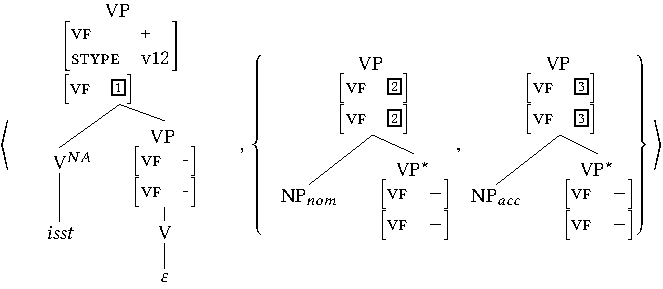
\includegraphics{graphics/abb76.pdf}
\caption{\label{fig-ttmctag-v12} Baumtupel für V1/V2-Sätze}
\end{figure} 
Bezogen auf den Kopfbaum entspricht der Wurzelknoten dem Vorfeld, der hiervon dominierte V-Knoten entspricht der linken Satzklammer, der Geschwisterknoten mit VP-Label entspricht dem Mittelfeld und schlie\ss lich der vom Mittelfeldknoten dominierte V-Knoten der rechten Satzklammer. Diese Zuordnung wird auch mittels des binären Merkmals {\sc vf} (für Vorfeld) angezeigt: Im {\sc top}-Bereich des Vorfeldknotens ist {\sc vf} $= +$, im Mittelfeldknoten {\sc vf} $= -$. Darüber hinaus wird ein unbesetztes Vorfeld dadurch angezeigt, dass der Vorfeldknoten den {\sc vf}-Wert des {\sc bottom}-Bereichs unspezifiziert lässt. Zur Durchsetzung der einmaligen Vorfeldbesetzung\is{Vorfeldbündelung} müssen die an VP adjungierende Elementarbäume, wie etwa die Argumentbäume des Tupels, in geeigneter Weise spezifiziert sein: Sie müssen (i) gewisserma\ss en erkennen, ob an ein bereits besetztes Vorfeld adjungiert werden soll oder nicht, und sie  müssen (ii) dafür Sorge tragen, dass nach der Adjunktion die Vorfeldbesetzung in den {\sc vf}-Merkmalen des Wurzelknotens angezeigt ist. Ersteres wird in Abbildung \ref{fig-ttmctag-v12} im Fu\ss knoten eines Hilfsbaums realisiert, der ja mit dem {\sc bottom}-Bereich des Zielknotens unifiziert und hier eine Verträglichkeit mit {\sc vf} $=-$ verlangt. Liegt eine Adjunktion an einem Vorfeldknoten vor, dann erreicht die Spezifizierung der Wertidentität der {\sc vf}-Merkmale im Wurzelknoten, dass nach der Adjunktion beide {\sc vf}-Merkmale des Wurzelknotens auf $+$ gesetzt sind. Damit ist eine weitere Adjunktion eines entsprechenden Hilfsbaums nicht mehr möglich, da dies zu einem Merkmalskonflikt führt. Abbildung \ref{fig-ttmctag-vorfeld2} stellt solch eine Situation dar. 
\begin{figure}[t]
\centering
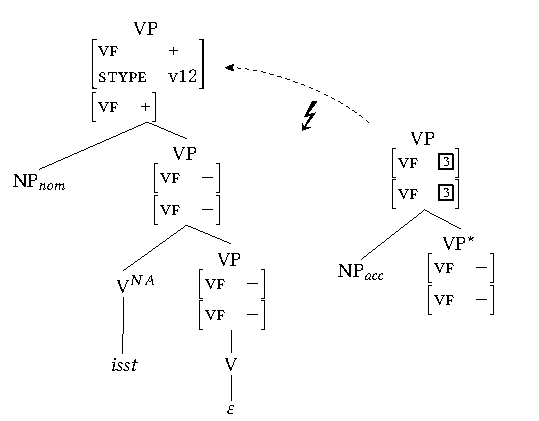
\includegraphics{graphics/abb77.pdf}
\caption{\label{fig-ttmctag-vorfeld2}Merkmalskonflikt bei mehrfacher Vorfeldbesetzung}
\end{figure} 
Im Unterschied zum Vorfeldknoten ist der Mittelfeldknoten so spezifiziert, dass auch mehrere Hilfsbäume sukzessiv adjungieren können.\footnote{Die Regulierung der Vorfeldbesetzung mit \textsc{vf} funktioniert im Prinzip so wie bei \citeauthor{Gerdes:02b} (\citeyear{Gerdes:02}; \citeyear[Section~4.3.2]{Gerdes:02b}). Nur komme ich ohne ein zusätzliches Merkmal (\textsc{novf}) aus, das Gerdes für einen bestimmten Sonderfall ("`un ou plus"', \citealt[Figure~126, 178]{Gerdes:02b}) benötigt, der aber meiner Ansicht nach bei Vorfeldern gar nicht eintritt. Außerdem wird bei meiner Analyse wert darauf gelegt, dass die Mittelfeldknoten kein positives \textsc{vf}-Merkmal besitzen. Rein kombinatorisch würde es schon ausreichen, nur den Vorfeldknoten entsprechend zu spezifizieren.}  

Für die Modellierung der Verbletztstellung\is{Satz!VE-}, bei der das finite Verb in der rechten Satzklammer steht und kein Vorfeld existiert, wird das Tupel in Abbildung \ref{fig-ttmctag-v3} verwendet. Es unterscheidet sich folgerichtig nur bezüglich der Form des Kopfbaumes von dem Tupel in Abbildung \ref{fig-ttmctag-v12}.   

\begin{figure}[t]
\centering
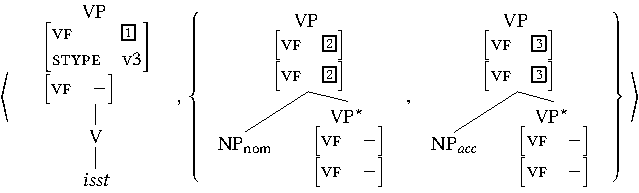
\includegraphics{graphics/abb78.pdf}
\caption{\label{fig-ttmctag-v3}Baumtupel für VE-Sätze}
\end{figure} 

Zuletzt möchte ich noch ein Schlaglicht auf die Modellierung der \isi{Komplementierer} von Verbletztsätzen\is{Satz!VE-} werfen, um zu verdeutlichen, warum sie in diesem TT-MCTAG-Ansatz topologisch weder der linken Satzklammer noch dem Vorfeld zuzuordnen sind. Der Komplementierer {\it dass} erhält grob den Elementarbaum in Abbildung~\ref{fig-ttmctag-comp}. Darin sorgt wiederum das binäre Merkmal {\sc vf} dafür, dass kein anderes Satzglied dem Komplementierer vorangestellt wird, während das  Merkmal {\sc stype} die Kombination mit VE-Sätzen sicherstellt.

\begin{figure}[t]
\centering
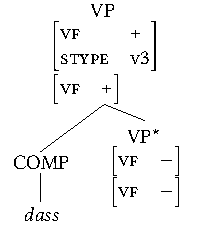
\includegraphics{graphics/abb79.pdf}
\caption{\label{fig-ttmctag-comp}Kopfbaum für \emph{dass}-Komplementierer}
\end{figure} 
  

\subsection{Stellungen des Verbalkomplexes}

Ich beschränke mich hier auf Verbalkomplexe\is{Verbalkomplex} mit drei Elementen und verwende die in Abschnitt \ref{sec-kohaerenz-einf} eingeführten Rangschemata mit schlussfeldbezogenem Index. Ich abstrahiere damit von den konkreten Status und Statusrektionen der beteiligten Verben. Des weiteren wird zunächst von den Argumentbäumen abgesehen.

%\subsubsection*{Grundstellung}

Die Grundstellung\is{Verbalkomplex!Grundstellung} entspricht dem Rangschema $V_3 V_2 V_1$, wobei $V_1$ für das ranghöchste, potenziell finite Verb und $V_3$ für das rangniedrigste Verb steht. Zur Derivation dieser Grundstellung werden die Elementarbäume in Abbildung \ref{fig-ttmctag-grund} eingesetzt. Die statusregierenden Verben werden als Hilfsbäume repräsentiert, in deren Fu\ss knoten der Status des regierten Verbs mittels des Merkmals {\sc stat(us)} spezifiziert ist. Die Spezifizierung des jeweils eigenen Status findet dagegen im Wurzelknoten platz. %Man beachte, dass hier angepasste {\sc stat}-Werte zu sehen sind, die sich von denen in der konkreten Grammatikimplementierung unterscheiden.
\begin{figure}[t]
\centering
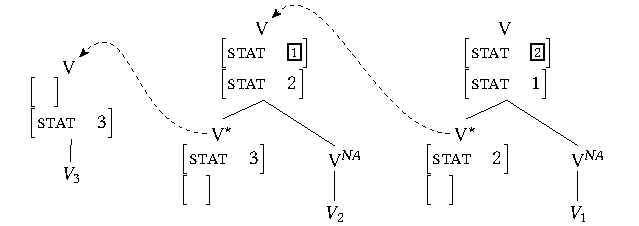
\includegraphics{graphics/abb710.pdf}
\caption{\label{fig-ttmctag-grund}Kopfbäume für die Grundstellung im Verbalkomplex}
\end{figure}


%\subsubsection*{Oberfeldumstellung}
\is{Verbalkomplex!Oberfeldumstellung|(}

Für die Derivation der Oberfeldumstellung $V_1 V_3 V_2$  müssen zwei Änderungen an den Elementarbäumen in Abbildung~\ref{fig-ttmctag-grund} vorgenommen werden: (i) der Fu\ss knoten des $V_1$-Baums muss rechtsperipher liegen, da sich das statusregierte Verb rechts von $V_1$ befindet; (ii) ein binäres Merkmal {\sc of} ist notwendig, um die Mindestgrö\ss e des Unterfelds\is{Verbalkomplex!Unterfeld} von zwei Verben wahren zu helfen. Beide Änderungen ergeben für die Derivation der Oberfeldumstellung die Elementarbäume in Abbildung~\ref{fig-ttmctag-ober}. Würde hier der $V_1$-Baum direkt am $V_3$-Baum adjungieren, dann würde das zu einem Konflikt der jeweiligen \textsc{of}-Merkmale führen (abgesehen vom Konflikt der \textsc{stat}-Merkmale). Erst der intervenierende $V_2$-Baum trägt ein kompatibles \textsc{of}-Merkmal.\footnote{Das {\sc of}-Merkmal entspricht dem \textsc{puf}-Merkmal in der HPSG-Analyse\is{Head-driven Phrase Structure Grammar (HPSG)} von \citet[201]{Meurers:99}. Zum \textsc{flip}-Merkmal bei \cite{Hinrichs:Nakazawa:94} besteht zwar auch eine gewisse funktionale Ähnlichkeit, aber anders als das \textsc{flip}-Merkmal löst das \textsc{of}-Merkmal die Oberfeldumstellung nicht direkt aus. Siehe \citet[201]{Meurers:99} für eine Gegenüberstellung von \textsc{flip} und \textsc{puf}.}   

\begin{figure}[t]
\centering
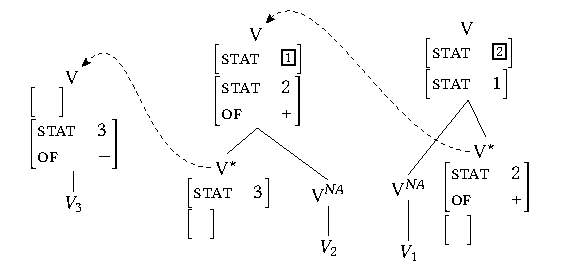
\includegraphics{graphics/abb711.pdf}
\caption{\label{fig-ttmctag-ober}Elementarbäume für die Oberfeldumstellung im Verbalkomplex}
\end{figure}

Die Oberfeldregel\is{Verbalkomplex!Oberfeldregel}, nach der das Oberfeld\is{Verbalkomplex!Oberfeld} kein Verb im 2.~Status enthält (siehe S.\,\pageref{ex-ofr}), wird in der TT-MCTAG-Modellierung durch das Fehlen entsprechender Oberfeld-Elementarbäume für Status-2-Verben implementiert.

Eine Verbalstellung wie $V_2 V_4 V_3 V_1$, in der die Oberfeldumstellung $V_2 V_4 V_3$ durch ein rechtsadjazentes $V_1$ zerstört wird, kann dagegen durch ein spezielles Merkmal verhindert werde, das die Adjunktion von $V_1$ an den Wurzelknoten von $V_2$ blockiert. Ich verzichte hier auf ein ausführliches Beispiel.
\is{Verbalkomplex!Oberfeldumstellung|)}


%\subsubsection*{Zwischenstellung}
\is{Verbalkomplex!Zwischenstellung}

Das wesentliche Merkmal der Zwischenstellung $V_3 V_1 V_2$ ist die lineare Einbettung eines ranghöheren Verbs zwischen rangniedrigeren Verben. Wenn entsprechend der Hilfsbaum von $V_2$ an $V_3$ und der Hilfsbaum von $V_1$ wiederum an $V_2$ adungieren soll, ist im Hilfsbaum von $V_2$ der Abbildungen~\ref{fig-ttmctag-grund} und~\ref{fig-ttmctag-ober} ein Präterminal ohne NA-Beschränkung\is{Adjunktionsbeschränkung} notwendig. Diese Anpassung ist in Abbildung~\ref{fig-ttmctag-zwisch} vorgenommen. $V_1$ kann nun alternativ an dem Knoten mit Gorn-Adresse 2 adjungiern und so die Zwischenstellung erzeugen. In diesem Knoten enthält das {\sc bottom}-Merkmal {\sc stat} den Status von $V_2$. Die Spezifizierung der Merkmalsidentität mittels \svar{3} dient hier dazu, die Adjunktion eines weiteren $V_1$-Verbs am Wurzelknoten von $V_2$ auszuschlie\ss en: Adjungiert $V_1$ am unteren Knoten, so kann keine weitere Instanz von $V_1$ am Wurzelknoten adjungieren (und vice versa), da es andernfalls zu einem Merkmalskonflikt bei {\sc stat} kommt.          

\begin{figure}[t]
\centering
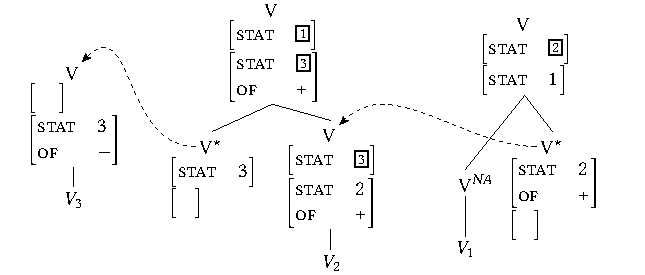
\includegraphics{graphics/abb712.pdf}
\caption{\label{fig-ttmctag-zwisch}Kopfbäume für die Zwischenstellung im Verbalkomplex}
\end{figure}




\subsection{Diskontinuierliche Kohärenzfelder}\label{sec-ttmctag-permutation}\is{Kohärenzfeld}

Zunächst soll auf die Grundstellung oder Intraposition der Kohärenzfeldtopologie eingegangen werden. Abweichungen hiervon folgen dann im Anschluss. Dieser Phänomenbereich wurde in Abschnitt~\ref{sec-permutation-kohaerenzfeld} ausführlich vorgestellt. Anders als bei der schematischen Darstellung der Implementierung von Verbalkomplexpermutationen empfiehlt sich hier die Verwendung konkreteren Anschauungsmaterials.

\subsubsection*{Grundstellung/Intraposition}\is{kohärente Konstruktion!Intraposition|(}

Die Intraposition des regierten Verbs eines Kohärenzfelds mit finitem Verb ist in \ref{ex-ttmctag-intra} zu sehen. \ref{ex-ttmctag-intra-b} zeigt eine Verbletzt"=Satzstellung und \ref{ex-ttmctag-intra-a} eine Verbzweit-Satzstellung.

\ex. \label{ex-ttmctag-intra}
\a. dass den Kühlschrank Peter zu reparieren versucht \label{ex-ttmctag-intra-b}
\b. Den Kühlschrank versucht Peter zu reparieren. \label{ex-ttmctag-intra-a}

Zur Modellierung der Verbletzt"=Stellung setze ich die Tupel in Abbildung~\ref{fig-ttmctag-koh2} ein. Das Schema der Kopfbäume sollte aus dem vorangegangenem Abschnitt über Verbalkomplexe vertraut sein. Die dort eingeführten Merkmale fehlen hier und im Weiteren der Übersichtlichkeit halber. Dagegen kommt nun ein neues binäres Merkmal {\sc phrase} zum Vorschein, das den phrasalen Status eines Knotens anzeigt. Im Wesentlichen dient es dazu, unechte Ambiguität zu vermeiden, ohne dabei das Lexikon aufzublähen.\footnote{Vergleichbares leistet in manchen HPSG-Modellen\is{Head-driven Phrase Structure Grammar (HPSG)}, z.\,B.\ in dem von \cite{Hinrichs:Nakazawa:94}, ein {\sc lex}-Merkmal (siehe \citealt{Mueller:96b,Mueller:97, Meurers:99b}). Man beachte, dass es sich bei diesen Modellen um Valenzvereinigungsansätze handelt.} Wie in Abbildung~\ref{fig-ttmctag-koh2} zu sehen, ist der Wurzelknoten von {\it zu reparieren} hinsichtlich {\sc phrase} unterspezifiziert, wodurch hier sowohl ein Argumentbaum (mit {\sc phrase} $ = +$) als auch {\it versucht} (mit {\sc phrase} $ = -$) adjungieren können. Zugleich ermöglicht die Unterscheidung qua {\sc phrase} die kontinuierliche Derivation des \isi{Verbalkomplex}, an dessen Wurzelknoten sukzessive die Restfeldglieder adjungieren. Dies ist im Ableitungsbaum darin zu erkennen, dass der Verbalkomplex einen verbundenen Teilbaum bildet. Eine unechte derivationelle Ambiguität durch die Alternation von links- und rechtsverzweigenden Hilfsbäumen wird somit an dieser Stelle verhindert. 

\begin{figure}[p]
\centering
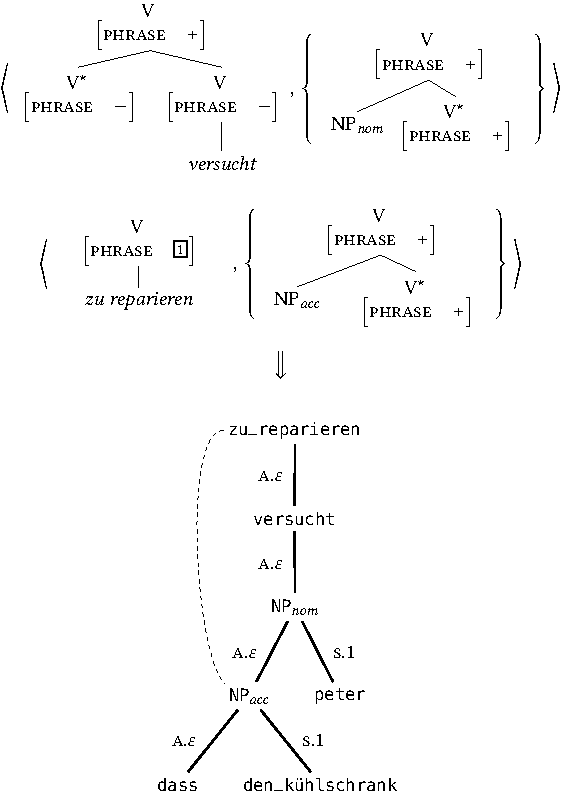
\includegraphics{graphics/abb713.pdf}
\caption{\label{fig-ttmctag-koh2}TT-MCTAG-Ableitung der Intraposition bei Verbletzt"=Satzstellung in Satz \ref{ex-ttmctag-intra-b}}
\end{figure}

Für eine bessere Lesbarkeit werde ich im Folgenden auf eine explizite Erwähnung des {\sc phrase}-Merkmals verzichten und stattdessen die implizite Notation in \ref{ex-ttmctag-notation} anwenden: 

\ex. \label{ex-ttmctag-notation}
\begin{tabular}[t]{ccl}
VP & $\approx$ & \begin{minipage}{7em}\begin{avm}\[phrase & +\]\end{avm}\end{minipage} \\[2ex] 
V & $\approx$ & \begin{minipage}{7em}\begin{avm}\[phrase & $-$\]\end{avm}\end{minipage} \\[2ex]
V(P) & $\approx$ & \begin{minipage}{7em}\begin{avm}\[ phrase & \@2\] \end{avm} \\ \begin{avm} \[phrase & \@1\]\end{avm}\end{minipage}
\end{tabular}

Daran hält sich auch die Darstellung der Tupel für die Derivation der Verbzweit-Stellung\is{Satz!V2-} von \ref{ex-ttmctag-intra-a} in Abbildung~\ref{fig-ttmctag-koh1}. Man erkennt au\ss erdem, dass der Kopfbaum des {\it versucht}-Tupels die Form des Kopfbaums des {\it isst}-Tupels aus Abbildung~\ref{fig-ttmctag-v12} wiederaufnimmt und durch einen Fu\ss knoten an der rechten Satzklammer erweitert. Der Rest bleibt verglichen mit Abbildung~\ref{fig-ttmctag-koh2} unverändert.

\begin{figure}[t]
\centering
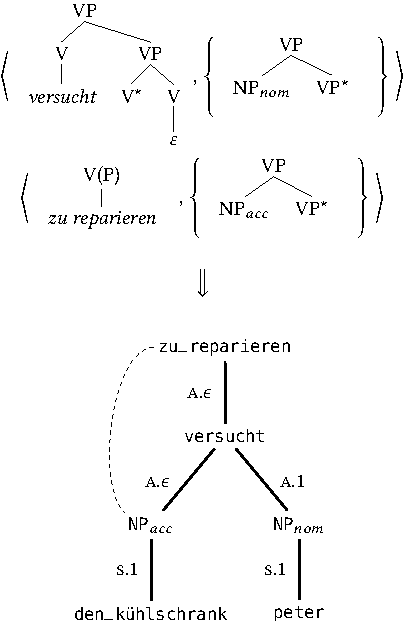
\includegraphics{graphics/abb714.pdf}
\caption{\label{fig-ttmctag-koh1}TT-MCTAG-Ableitung der Intraposition bei Verbzweit"=Satzstellung in Satz \ref{ex-ttmctag-intra-a}}
\end{figure}

Der Kopfbaum des {\it versucht}-Tupels in Abbildung~\ref{fig-ttmctag-koh1} lässt jedoch bereits eine gravierende Einschränkung dieser TT-MCTAG-Analyse erkennen: Die Argumentbäume der statusregierten Verben können nach Vorgabe der Node-Sharing-Lokalität\is{Node Sharing} nicht an seinem Mittelfeldknoten adjungieren, da dieser kein Wurzelknoten des Kopfbaums ist. Das \isi{Scrambling} von Ergänzungen unterschiedlicher Verbalfelder im Mittelfeld ist dadurch nicht abgedeckt. Dazu mehr in Abschnitt~\ref{sec-ttmctag-grenzen}.
\is{kohärente Konstruktion!Intraposition|)}

% \begin{figure}[ht]
% \begin{center}
% 
% $\left <
% \mbox{
% \begin{tabular}{cc}
% \multicolumn{2}{c}{\node{0}{VP}} \\[2ex]
% \node{1}{V} & \node{2}{VP*} \\[2ex]
% \node{11}{{\tt hat}}
% \end{tabular}
% \nodeconnect{0}{1} \nodeconnect{0}{2}
% \nodeconnect{1}{11}
% \hspace{-2em} , %%%
% $\left \{
% \right \}$
% }
% \right >$
% 
% $\left <
% \mbox{
% \begin{tabular}{cc}
% \multicolumn{2}{c}{\node{0}{V(P)}} \\[2ex]
% \node{1}{V*} & \node{2}{V} \\[2ex]
%  & \node{21}{{\tt versucht}}
% \end{tabular}
% \nodeconnect{0}{1} \nodeconnect{0}{2}
% \nodeconnect{2}{21}
% \hspace{-2em} , %%%
% $\left \{
% \mbox{
% \begin{tabular}{cc}
% \multicolumn{2}{c}{\node{vps0}{VP}} \\[2ex]
% \node{vps1}{NP$_{nom}\!\downarrow$} & \node{vp2}{VP*} \\[2ex]
% \end{tabular} %\\[4ex]
% \nodeconnect{vps0}{vps1}
% \nodeconnect{vps0}{vp2}
% }
% \right \}$
% }
% \right >$
% 
% $\left <
% \mbox{
% \begin{tabular}{c}
% \node{0}{V(P)} \\[2ex]
% \node{1}{{\it zu reparieren}}
% \end{tabular}
% \nodeconnect{0}{1}
% , %%%
% $\left \{
% \mbox{
% \begin{tabular}{cc}
% \multicolumn{2}{c}{\node{vpo0}{VP}} \\[2ex]
% \node{vpo1}{NP$_{acc}\!\downarrow$} & \node{vp2}{VP*} \\[2ex]
% \end{tabular} %\\[4ex]
% \nodeconnect{vpo0}{vpo1}
% \nodeconnect{vpo0}{vp2}
% }
% \right \}$
% }
% \right >$
% 
% \bigskip
% 
% \rotatebox{90}{$\Longleftarrow$}
% 
% \bigskip
% 
% \pstree[nodesep=3pt,levelsep=1.5cm]{\Tr{\node{head}{{\tt zu\_reparieren}}}}{% 
%   \pstree{\Tr{{\tt versucht}}\tlput{a.0}}{
%     \pstree{\Tr{{\tt NP$_{nom}$}}\tlput{a.0}}{
%       \pstree{\Tr{\node{arg}{{\tt hat}}}\tlput{a.0}}{
%         \pstree{\Tr{\node{arg}{{\tt NP$_{acc}$}}}\tlput{a.0}}{\Tr{{\tt den\_kühlschrank}}\trput{s.1}}
%       }
%       \Tr{{\tt peter}}\trput{s.1}
%     }
%   }
% }
% {\makedash{2pt}
% \nodecurve[l]{head}[l]{arg}{30pt}
% }
% 
% \end{center}
% \caption{\label{fig-ttmctag-koh3}  }
% \end{figure}


% \ex. 
% \a. Den Kühlschrank hat Peter zu reparieren versucht.
% \b. dass den Kühlschrank Peter zu reparieren versucht hat.


\subsubsection*{3.~Konstruktion}\is{kohärente Konstruktion!3.~Konstruktion|(}

Die Herausforderung der 3.~Konstruktion besteht in dem Nebeneinander von kohärenten und inkohärenten topologischen Bereichen bei zwei Verbfeldern $V^i$, $V^{i+1}$: der inkohärente Bereich ist zwar für die Bestandteile von $V^{i+1}$ zugänglich, aber die Bestandteile des regierenden Verbalfeldes $V^i$ sind hiervon ausgeschlossen; zum anderen gibt es kohärente Bereiche, zu denen die Bestandteile beider Verbalfelder prinzipiell gleicherma\ss en Zugang haben. Deutlich wird dies an den Beispielen in \ref{ex-ttmctag-extra}. Die Ergänzung {\it den Kühlschrank} des extraponierten regierten Verbs {\it zu reparieren} kann zwar sowohl im Mittelfeld der extraponierten VP als auch im Mittelfeld des Matrixsatzes platziert werden, wie \ref{ex-ttmctag-extra-a} und \ref{ex-ttmctag-extra-b} zeigen, die \isi{Extraposition} der Ergänzung des ranghöheren Finitums {\it Peter} zusammen \textit{zu reparieren} ist dagegen unzulässig (vgl.\ \ref{ex-ttmctag-extra-c}): 

\ex. \label{ex-ttmctag-extra}
\a. dass Peter den Kühlschrank versucht, zu reparieren. \label{ex-ttmctag-extra-a}
\b. dass Peter versucht, den Kühlschrank zu reparieren. \label{ex-ttmctag-extra-b}
\c. *dass den Kühlschrank versucht, Peter zu reparieren. \label{ex-ttmctag-extra-c}

Die TT-MCTAG-Modellierung der 3.~Konstruktion muss also erreichen, dass die rechtsverzweigenden Argumentbäume von {\it versucht} nicht in einem Bereich adjungieren, der extraponiert ist (bzw.\ im \isi{Nachfeld} steht).\footnote{Selbstverständlich können bestimmte Ergänzungen finiter Verben extraponiert werden; sie sind dann aber unmittelbare Bestandteile des Nachfelds und nicht im Kohärenzfeld eines regierten Verbs eingebettet. Im Rahmen einer TT-MCTAG-Theorie der Extraposition kann das mittels linksverzweigender Argumentbäume modelliert werden.} Dafür ist tatsächlich nicht viel zu tun: Die Hinzunahme des Tupels für {\it versucht} in Abbildung \ref{fig-ttmctag-3konstr} reicht dafür aus. Der Fu\ss knoten steht hier gleichsam für den extraponierten Teil des regierten Verbalfelds. Dank der Beschränkung durch die Node-Sharing-Lokalität\is{Node Sharing} ist es nicht möglich, einen Argumentbaum von {\it versucht} "`unterhalb"' des Fu\ss knotens zu adjungieren.\footnote{Eine entscheidende Rolle spielt dabei natürlich auch die generelle NA-Beschränkung\is{Adjunktionsbeschränkung} auf den Fu\ss knoten.} Stattdessen muss die Adjunktion am Wurzelknoten oder "`darüber"' erfolgen. 


\begin{figure}[t]
\centering
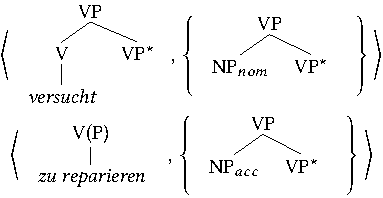
\includegraphics{graphics/abb715.pdf}
\caption{\label{fig-ttmctag-3konstr}Baumtupel für die Ableitung der 3.~Konstruktion in \ref{ex-ttmctag-extra}}
\end{figure}

Was das extraponierte Verb {\it zu reparieren} betrifft, können seine Argumentbäume entsprechend der Node-Sharing-Lokalität\is{Node Sharing} entweder "`zwischen"' dem Wurzelknoten von {\it zu reparieren} und dem Fu\ss knoten von {\it zu versuchen} adjungieren, oder "`oberhalb"' des Wurzelknotens von {\it zu versuchen}, in gleicher Weise wie die Argumentbäume von {\it zu versuchen}. Damit wird die Verteilungsasymmetrie der Er\-gän\-zungen erfasst. 

Leider können nicht alle Instanzen der 3.~Konstruktion erfasst werden, ohne wesentlich von den bis hierhin befolgten Designrichtlinien abzuweichen. Zwar erwachsen bei Verbletzt-Sätzen wie \ref{ex-ttmctag-extra} keine Schwierigkeiten, doch erweisen sich Verbzweit-Sätze\is{Satz!V2-} wie \ref{ex-ttmctag-extra2} als problematisch: 

\ex. Peter fängt den Kühlschrank an zu reparieren. \label{ex-ttmctag-extra2}

Dies erinnert an die Bemerkung am Ende des letzten Abschnitts: Wieder ist es ein im Elementarbaum nicht als Wurzelknoten realisierter und deshalb nicht er"-reichbarer Mittelfeldknoten, der eine umfassende Modellierung verhindert. Wir werden uns damit im Detail in Abschnitt~\ref{sec-ttmctag-grenzen} auseinandersetzen. Diese Einschränkung wird bei der Voranstellung, zu der wir nun kommen, noch deutlicher, da sie ausschlie\ss lich in V2-Sätzen auf"|tritt.
\is{kohärente Konstruktion!3.~Konstruktion|)}       


\subsubsection*{Partielle Voranstellung}\is{Voranstellung!partielle|(}

Vergleichbar der Extraposition zeigt auch die Voranstellung regierter Verben ins \isi{Vorfeld} ein Nebeneinander von Kohärenz und Inkohärenz. Die Ergänzung des vorangestellten infiniten Verbs {\it zu reparieren} kann sowohl vorangestellt sein wie in \ref{ex-ttmctag-front-a} als auch im Mittelfeld auf"|tauchen wie in \ref{ex-ttmctag-front-b}. Diese distributionelle Freiheit hat die Ergänzung des Finitums, {\it Peter}, dagegen nicht, vgl.\ \ref{ex-ttmctag-front-c}: 

\ex. \label{ex-ttmctag-front}
\a. Den Kühlschrank zu reparieren versucht Peter. \label{ex-ttmctag-front-a}
\b. Zu reparieren versucht Peter den Kühlschrank. \label{ex-ttmctag-front-b}
\c. *Peter zu reparieren versucht den Kühlschrank. \label{ex-ttmctag-front-c}

Für die Modellierung der vollständigen Voranstellung in \ref{ex-ttmctag-front-a} wird wieder ein zusätzliches Tupel für das regierende Verb eingesetzt. Der Kopfbaum von {\it versucht} in Abbildung~\ref{fig-ttmctag-front} entspricht dem Elementarbaum eines Finitums für die V1- und V2-Satzstellung\is{Satz!V1-}\is{Satz!V2-}, ergänzt durch einen linksperipheren Fu\ss knoten für eine regierte Verbalphrase.

\begin{figure}[t]
\centering
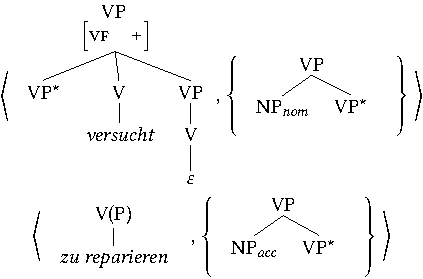
\includegraphics{graphics/abb716.pdf}
\caption{\label{fig-ttmctag-front}Baumtupel für die Ableitung der VP-Voranstellung in \ref{ex-ttmctag-front}}
\end{figure}

Die mit den Tupeln in Abbildung~\ref{fig-ttmctag-front} erfasste Voranstellung ist zwangsläufig vollständig, denn die Argumentbäume des vorangestellten Verbs können nicht am Mittelfeldknoten des {\it versucht}-Kopfbaums adjungieren. Gemä\ss\ der Node"=Sharing"=Lokalität\is{Node Sharing} ist nämlich nur der Wurzelknoten eines an den Kopfbaum adjungierenden Hilfsbaums erreichbar. Wie können aber Instanzen einer partiellen Voranstellung wie \ref{ex-ttmctag-front-b} modelliert werden? Die unbefriedigende Antwort lautet: wohl nicht ohne wesentliche Änderungen an den Designprinzipien. An diesem Punkt erleben wir, dass durch die überschneidenden Geltungsbereiche von Node"=Sharing-Lokalität, Valenzprinzip\is{Wohlgeformtheitsprinzip!Valenzprinzip} und Annahme einer rechtsverzweigenden Phrasenstruktur\is{Phrasenstruktur!rechtsverzweigende} technische Grenzen gesetzt sind, die bei der partiellen Voranstellung überschritten werden. In Abschnitt~\ref{sec-ttmctag-grenzen} werde ich auf diese Grenze und mögliche Auswege genauer eingehen.

Was die Voranstellung von Subjekten\is{Subjekt} bzw.\ Nominativ-NPs mit einer infiniten Verbalphrase betrifft, z.\,B.\ in \ref{ex-ttmctag-part-1}, werde ich in Abschnitt~\ref{sec-ttmctag-rekt} einen Mechanismus mit indirekter Kasusmarkierung (d.\,h.\ mittels \isi{Merkmalsperkolation} in der syntaktischen Struktur) implementieren, der aus der üblichen TAG-Analyse von Anhebungskonstruktionen\is{Anhebung} \citep[Chapter~9]{xtag:01} übernommen und auch bei der Analyse des Fernpassivs\is{Passiv!Fern-} verwendet werden kann:    

\ex. \label{ex-ttmctag-part-1} Ein Au\ss enseiter zu gewinnen scheint hier eigentlich nie. \\ 
\citep[(265)]{Meurers:99}

Dieses Vorgehen setzt sich deutlich von Analysevorschlägen im Rahmen der HPSG\is{Head-driven Phrase Structure Grammar (HPSG)} ab, wo die \isi{Kasusmarkierung} anhand der Valenzinformationen in der {\sc subcat}"=Liste vollzogen wird \citep{Heinz:Matiasek:94,Meurers:99,Mueller:01}. 
 
Noch eine Bemerkung zur ternären Phrasenstruktur\is{Phrasenstruktur} des Voranstellungsbaums in Abbildung~\ref{fig-ttmctag-front}: Hier wird aus Ökonomiegründen vom binären Phrasenstrukturschema in Abbildung~\ref{fig-ttmctag-ps-1} (S.\,\pageref{fig-ttmctag-ps-1}) abgewichen. Die Implementierung einer binären Struktur wäre zwar ohne Weiteres möglich, aber dann gäbe es einen internen Vorfeldknoten mit NA-Beschränkung\is{Adjunktionsbeschränkung}, an den nichts adjungieren könnte, der also aus kombinatorischer Sicht bedeutungslos wäre. Solche Knoten sind an sich unschädlich, widersprechen aber dem Ökonomieprinzip\is{Wohlgeformtheitsprinzip!Oekonomieprinzip@Ökonomieprinzip} (siehe S.\,\pageref{ex-oekonomieprinzip-tag}). 
\is{Voranstellung!partielle|)}

\subsubsection*{Linksstellung}\is{Linksstellung}

Wie in Abschnitt~\ref{sec-linksstellung} beschrieben, sind zwei Formen der Linksstellung zu unterscheiden. Zum einen kann das Oberfeld\is{Verbalkomplex!Oberfeld} in das Mittelfeld verschoben sein, wie in Beispiel \ref{ex-ttmctag-links1-a} das finite Hilfsverb {\it hat}:\is{Linksstellung!des Oberfelds}

\ex. \label{ex-ttmctag-links1}
\a. dass Peter den Kühlschrank hat neulich reparieren lassen \label{ex-ttmctag-links1-a}
\b. dass Peter den Kühlschrank hat müssen neulich reparieren lassen \label{ex-ttmctag-links1-b}
\c. *dass hat Peter den Kühlschrank neulich reparieren lassen \label{ex-ttmctag-links1-c}

Satz \ref{ex-ttmctag-links1-b} beweist, dass das linksversetzte Oberfeld tatsächlich auch mehrgliedrig sein kann. Und Satz \ref{ex-ttmctag-links1-c} zeigt schlie\ss lich, dass das linksversetzte Oberfeld nicht adjazent zum \isi{Komplementierer} stehen kann. In Abschnitt~\ref{sec-linksstellung} wurde letztere Einsicht als Linksstellungsregel bezeichnet. 

Zum anderen besteht die Möglichkeit, das maximal untergeordnete Verb\is{Linksstellung!des maximal untergeordneten Verbs} einer kohärenten subordinativen Kette im Mittelfeld zu platzieren. Vermutlich ist dies jedoch auf Verben mit 2.~Status beschränkt. Beispiele hierfür finden sich in \ref{ex-ttmctag-links2}:

\ex. \label{ex-ttmctag-links2}
\a. Den Kühlschrank hat er zu reparieren noch nicht versucht. \label{ex-ttmctag-links2-a}
\b. dass zu reparieren Peter den Kühlschrank nicht versucht hat \label{ex-ttmctag-links2-b}


\is{Linksstellung!des Oberfelds|(}
Wenden wir uns zunächst der TT-MCTAG-Analyse der Oberfeld-Links\-stel\-lung (OF-Links\-stellung) zu. Hier beschränke ich mich auf OF-Linksstellungen mit einstelligem Oberfeld wie in \ref{ex-ttmctag-links1-a}, um die Darstellung einfach zu halten.\footnote{Mehrgliedrige linksversetzte Oberfelder können mit geeigneten Merkmalen in der VP-Projektion des Mittelfelds modelliert werden. Die Ausbuchstabierung dessen fügt an diesem Punkt  der TT-MCTAG-Analyse kohärenter Konstruktionen keinen neuen Aspekt hinzu.} Abbildung~\ref{fig-ttmctag-links1} enthält die entsprechenden Kopfbäume der verbalen Tupel.  
\begin{figure}[t]
\centering
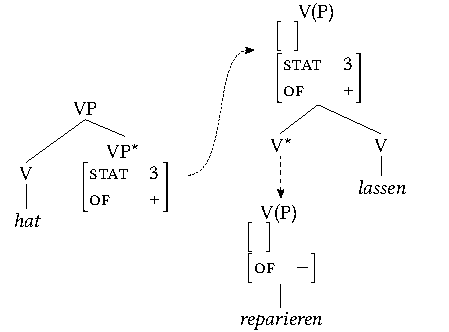
\includegraphics{graphics/abb717.pdf}
\caption{\label{fig-ttmctag-links1}Kopfbäume für die Ableitung der Oberfeld-Linksstellung in \ref{ex-ttmctag-links1}. Der gepunktete Pfeil vom {\it hat}-Baum zum {\it lassen}-Baum drückt ein Dominanzverhältnis im abgeleiteten Baum aus.}
\end{figure}
Neu ist hieran der Elementarbaum des linksversetzten {\it hat}: Im Unterschied zum $V_1$-Elementarbaum des Oberfeldschemas in Abbildung~\ref{fig-ttmctag-ober} adjungiert {\it hat} an einen VP-Knoten. Au\ss erdem wird bei der Analyse in Abbildung~\ref{fig-ttmctag-links1} implizit angenommen, dass das {\sc of}-Merkmal und das {\sc stat}-Merkmal in der VP-Projektion weitergereicht werden. Dies reicht aus, um zu erreichen, dass beliebiges Material des Mittelfelds zwischen Oberfeld und Unterfeld intervenieren kann. Aufgrund der Node-Sharing-Lokalität\is{Node Sharing} sind jedoch die Argumentbäume des linksversetzten Verbs, hier die Nominativ"=NP, zu solch einer Intervention unfähig, da sie in diesem Fall nicht mittelbar am Kopfbaum adjungieren. Diese Einschränkung deckt sich leider nicht mit dem empirischen Befund, demzufolge die Nominativ-NP sehr wohl Teil des intervenierenden Restfeldmaterials sein kann. Dazu gehört z.\,B.\ \ref{ex-ttmctag-links3}: 

\ex. \label{ex-ttmctag-links3} Da\ss\ ihn gestern hätte jemand besiegen können, ist unwahrscheinlich. \\
(Wiederholung von \ref{ex-meurers-146b}, S.\,\pageref{ex-meurers-146b})

Was die Linksstellungsregel betrifft, nach der das linksversetzte Oberfeld nicht adjazent zum \isi{Komplementierer} stehen darf, reicht wiederum der unspektakuläre Einsatz entsprechender Merkmale in der VP-Projektion aus. Ich übergehe hier eine detaillierte Darstellung.
\is{Linksstellung!des Oberfelds|)}  

\is{Linksstellung!des maximal untergeordneten Verbs|(}
Die Linksstellung des maximal untergeordneten Verbs in \ref{ex-ttmctag-links2}, die ich in Abschnitt~\ref{sec-permutation-kohaerenzfeld} auch als Unterfeld-Linksstellung\is{Verbalkomplex!Unterfeld} bezeichnet habe, ist ungleich interessanter, weil für den hier vorgestellten TT-MCTAG-Ansatz problematischer. Der Satz \ref{ex-ttmctag-links2-a} ist dabei der einfachere und kann mittels der verbalen Kopfbäume in Abbildung~\ref{fig-ttmctag-links2-1} deriviert werden. Die Anpassung erfolgt am {\it versucht}"=Elementarbaum, indem dort der Geschwisterknoten des Fu\ss knotens für Restfeldmaterial zugänglich gemacht wird.   
\begin{figure}[t]
\centering
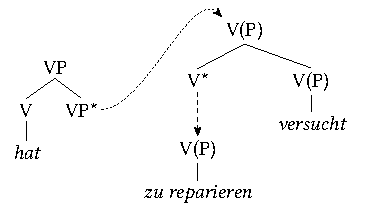
\includegraphics{graphics/abb718.pdf}
\caption{\label{fig-ttmctag-links2-1}Kopfbäume für die Ableitung der Unterfeld-Linksstellung in \ref{ex-ttmctag-links2-a}. Der gepunktete Pfeil vom {\it hat}-Baum zum {\it versucht}-Baum drückt ein Dominanzverhältnis im abgeleiteten Baum aus.}
\end{figure}
Dagegen entzieht sich Satz \ref{ex-ttmctag-links2-b} einer Derivation innerhalb der Grenzen des hier verfolgten TT-MCTAG-Ansatzes. Die verbalen Kopfbäume in Abbildung~\ref{fig-ttmctag-links2-2} sollten dies deutlich machen. Da hier eine Verbletzt"=Satzstellung vorliegt, adjungiert der {\it hat}-Elementarbaum an den Verbalkomplex in der rechten Satzklammer. Der kritische Punkt dieser Analyse ist wieder der optional phrasale Geschwisterknoten des Fu\ss knotens, an den unmittelbar oder mittelbar das intervenierende Restfeldmaterial adjungieren muss. Dem kann nämlich der Argumentbaum des linksversetzen Verbs {\it zu reparieren} nicht nachkommen, da diese Position nicht im Bereich der Node-Sharing-Lokalität\is{Node Sharing} liegt. Da eine Analysealternative, d.\,h.\ eine sinnvolle Anpassung der Elementarbäume, nicht verfügbar zu sein scheint, ist die Derivation von Satz \ref{ex-ttmctag-links2-b} nicht möglich. Es wiederholt sich also die Modellierungssackgasse, in die wir schon bei Fällen der 3.~Konstruktion und der partiellen Voranstellung geraten sind. Und wieder verweise ich auf Abschnitt \ref{sec-ttmctag-grenzen} für eine eingehende Untersuchung und das Ausloten von Modellierungsauswegen.     

\begin{figure}[t]
\centering
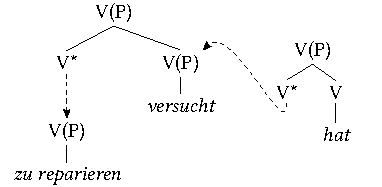
\includegraphics{graphics/abb719.pdf}
\caption{\label{fig-ttmctag-links2-2}Kopfbäume für die Ableitung der Unterfeld-Linksstellung in \ref{ex-ttmctag-links2-b}}
\end{figure}
\is{Linksstellung!des maximal untergeordneten Verbs|)}


\subsection{Rektionsbesonderheiten} \label{sec-ttmctag-rekt}

Interessant sind an dieser Stelle solche Rektionsbesonderheiten\is{Rektion}, die mit einer syntaktischen Beschränkung einhergehen, d.\,h.\ von der Position des Regens und des Rektums abhängig sind. Ich werde auf diesen Aspekt bei Ersatzinfinitiven, Ersatz-\emph{zu}-Infinitven und bei Fernpassiv-Konstruktionen eingehen. 

\subsubsection*{Ersatzinfinitiv}\is{Ersatzinfinitiv|(}

Die Existenz einer Ersatzinfinitivform bei bestimmten Verben wird durch die sogenannte Unterfeldregel\is{Ersatzinfinitiv!Unterfeldregel} (siehe S.\,\pageref{ex-ufr}) syntaktisch eingeschränkt, derzufolge das regierende Verb des Ersatzinfinitivs nicht im Unterfeld stehen darf.\footnote{Möglicherweise ist die Unterfeldregel zu strikt. Siehe S.\,\pageref{ex-ufr}f für eine kurze Diskussion.} Dadurch sind die Grammatikalitätsurteile in \ref{ex-ttmctag-ersatz} korrekt erfasst:

\ex. \label{ex-ttmctag-ersatz}
\a. *dass er heute Schokolade essen dürfen hat
\b. ?dass er heute Schokolade essen hat dürfen
\c. dass er heute Schokolade hat essen dürfen

Die Unterfeldregel kann im TT-MCTAG-Ansatz mittels eines binären Merkmals {\sc e-inf} implementiert werden, das die Existenz eines Ersatzinfinitivs anzeigt. Für das regierende Verb ist damit also sichtbar, ob das regierte Verb im Ersatzinfinitiv realisiert ist. Der Elementarbaum des regierenden Verbs für die Grundstellung\is{Verbalkomplex!Grundstellung} wird schlie\ss lich bezüglich {\sc e-inf} so spezifiziert, dass es mit der Existenz des Ersatzinfinitivs unverträglich ist. Dagegen sind die Elementarbäume des regierenden Verbs für die anderen Verbalkomplexstellungen\is{Verbalkomplex} bezüglich {\sc e-inf} unterspezifiziert.
\is{Ersatzinfinitiv|(}

\subsubsection*{Ersatz-\emph{zu}-Infinitiv}\is{Ersatz-\emph{zu}-Infinitiv|(}

Wie in Abschnitt \ref{sec-abweichung-rektion} (S.\,\pageref{ex-kohaerenz-zuersatz-1}) ausführlich dargestellt, muss die Modellierung des Ersatz-\emph{zu}-Infinitivs in \ref{ex-ttmctag-zuersatz-1-a} zwei Eigenschaften erfassen: (i) das ranghöchste Verb des Schlussfelds, {\it haben}, hat den 1.~Status anstelle des 2.~Status; (ii) das von {\it haben} regierte Verb trägt den 2.~Status anstelle des Ersatzinfinitivs. Die beiden zu erwartenden Alternativen in \ref{ex-ttmctag-zuersatz-1-b} und \ref{ex-ttmctag-zuersatz-1-c} werden durch die Oberfeldregel\is{Verbalkomplex!Oberfeldregel} bzw.\ durch die Unterfeldregel\is{Ersatzinfinitiv!Unterfeldregel} verhindert:

\ex. \label{ex-ttmctag-zuersatz-1}
\a. Ich glaube es haben$_1$ tun$_3$ zu können$_2$. \label{ex-ttmctag-zuersatz-1-a} 
\b. *Ich glaube es zu haben$_1$ tun$_3$ können$_2$. \label{ex-ttmctag-zuersatz-1-b}
\c. *Ich glaube es tun$_3$ können$_2$ zu haben$_1$. \label{ex-ttmctag-zuersatz-1-c}

Ich schlage hier eine TT-MCTAG-Modellierung vor, bei der ein zusätzlicher Elementarbaum für {\it haben} wie der in Abbildung~\ref{fig-ttmctag-ersatzzu} angenommen wird. Anders als das sonst gebrauchte infinite \isi{Hilfsverb} {\it haben}, regiert dieses {\it haben} einen Infinitiv im 2.~Status mit Ersatzinfinitiv-Marker\is{Markierer} (d.\,h.\ {\sc e-inf} $=$ +). Dieser Ersatzinfinitiv-Marker zeigt im Grunde die Ersatzinfinitiv-Fähigkeit eines Verbs an und wird lexikalisch bestimmt. Dadurch findet sich der auslösende Faktor für die Existenz der Ersatz-\emph{zu}-Infinitive tatsächlich alleine im dargestellten {\it haben}-Hilfsbaum.

\begin{figure}[t]
\centering
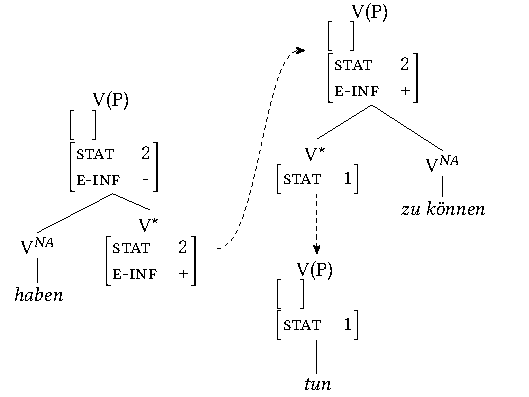
\includegraphics{graphics/abb720.pdf}
\caption{\label{fig-ttmctag-ersatzzu}Kopfbäume für die Ableitung des Ersatz-\emph{zu}-Infinitivs in \ref{ex-ttmctag-zuersatz-1-a}}
\end{figure}

Die Eigenart des TT-MCTAG-Ansatzes, für jede Abweichung von einem vermeintlichen Kernregularium einen zusätzlichen Elementarbaum (und folglich ein zusätzliches Tupel) zu stipulieren, mag auf den ersten Blick wenig attraktiv wirken, wenn man hier wie \cite{Bech:63} oder \cite{Vogel:09} das Dilemma zweier Stellungsregeln am Werk sieht, aus dem die Existenz des Ersatz-\emph{zu}-Infinitivs irgendwie hervorgehen soll. Diese Betrachtungsweise übersieht jedoch, dass an dieser Stelle irgendetwas zusätzlich stipuliert werden muss, denn stipulationsfrei wäre allein das Fehlen des Ersatz-\emph{zu}-Infinitivs zu erklären, wenn man die Bechsche Systematik zugrunde legt. Natürlich lässt sich trotzdem darüber streiten, wie die zusätzliche Stipulation beschaffen sein soll.\footnote{Allerdings bin ich der Meinung, dass man alternative Stipulationsmöglichkeiten nur bezüglich einer konkreten Implementierung in einem bestimmten Grammatikframework evaluieren kann. Nur bezüglich einer konkreten Implementierung kann man etwas über den Umfang einer Stipulation sagen und diesen mit dem Umfang anderer Stipulationen vergleichen. Es ist jedoch völlig hoffnungslos, etwa eine Implementierung der \isi{Optimalitätstheorie} oder der HPSG\is{Head-driven Phrase Structure Grammar (HPSG)} einer TT-MCTAG-Implementierung in ebensolcher Weise gegenüberzustellen. Oder mit anderen Worten: Es kann zwar verglichen werden, was Implementierungen unterschiedlicher Grammatikframeworks zu erfassen vermögen; es kann aber nicht verglichen werden, wie sie dies jeweils bewerkstelligen, ohne die Grundunterschiede der betroffenen Grammatikframeworks zu berücksichtigen.} Im Rahmen des TT-MCTAG-Ansatzes scheint es beispielsweise erstrebenswerter zu sein, statt eines weiteren Tupels "`nur"' ein weiteres Merkmal oder besser noch die Modifizierung eines bereits vorhandenen Merkmals zu stipulieren. Man könnte dahingehend annehmen, dass ein infinites {\it haben} im Oberfeld durch den Elementarbaum in Abbildung~\ref{fig-ttmctag-ersatzzu-2} repräsentiert wird.
\begin{figure}[t]
\centering
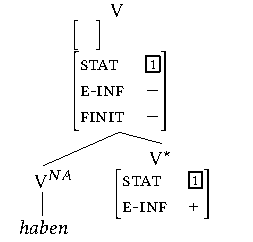
\includegraphics{graphics/abb721.pdf}
\caption{\label{fig-ttmctag-ersatzzu-2}Kopfbaum für {\it haben} im Oberfeld}
\end{figure}
Statt einer konkreten Statusspezifizierung wie in Abbildung~\ref{fig-ttmctag-ersatzzu} ist hier nur eine Identität zwischen dem regierten Status und dem Status des Verbalkomplexes\is{Verbalkomplex} spezifiziert. Au\ss erdem ist dieser {\it haben}-Elementarbaum weiterhin nur auf Verbalkomplexe mit Ersatzinfinitiv-Beteiligung anwendbar. Dadurch wird tatsächlich nicht nur die Durchlässigkeit für den Ersatzinfinitiv-Status in \ref{ex-ttmctag-zuersatz-3} erfasst, sondern auch die  Nichtverfügbarkeit der Oberfeldumstellung bei einem Fehlen des Ersatzinfinitivs, vgl.\ \ref{ex-ttmctag-zuersatz-2}:

\ex. \label{ex-ttmctag-zuersatz-3}
\a. Peter könnte den Kühlschrank haben reparieren lassen. \label{ex-ttmctag-zuersatz-3-a}
\b. ohne den Kühlschrank haben reparieren zu lassen \label{ex-ttmctag-zuersatz-3-a}

\ex. \label{ex-ttmctag-zuersatz-2}
\a. Peter könnte den Kühlschrank zu reparieren versucht haben. \label{ex-ttmctag-zuersatz-2-a}
\b. Peter könnte den Kühlschrank haben zu reparieren *versucht/*ver\-su\-chen. \label{ex-ttmctag-zuersatz-2-b} 

Dieser Ansatz hat starke Ähnlichkeiten zum HPSG-Ansatz\is{Head-driven Phrase Structure Grammar (HPSG)} von \citet[Section~8.2]{Meurers:99}, wo Oberfeld-Elemente als Marker\is{Markierer} modelliert werden, die zwar nicht die Statusinformationen der Verbprojektion (in {\sc vform}) beeinflussen, aber deren Finitheits"= und Kongruenzmerkmale abgreifen können. 
\is{Ersatz-\emph{zu}-Infinitiv|)}


\subsubsection*{Kasusrektion bei Fernpassiv und VP-Voranstellung} \label{sec-ttmctag-fern}

Abschlie\ss end möchte ich kurz auf die Modellierung des Fernpassivs und der Voranstellung von Subjekt (bzw.\ Nominativ-NP) und infinitem Verb eingehen. Beiden Phänomenen ist gemein, dass sie als eine Folge indirekter Kasusrektion modelliert werden.

\is{Passiv!Fern-|(} 
Die Sätze in \ref{ex-ttmctag-fern} exemplifizieren nochmals die wichtigsten Eigenschaften des Fernpassivs (siehe auch Abschnitt~\ref{sec-fernpassiv}, S.\,\pageref{sec-fernpassiv}):

\ex. \label{ex-ttmctag-fern}
\a. wenn Peter den Kühlschrank zu reparieren versucht \label{ex-ttmctag-fern-a}
\b. wenn der Kühlschrank von Peter zu reparieren versucht wird \label{ex-ttmctag-fern-b}
\c. wenn den Kühlschrank zu reparieren versucht wird \label{ex-ttmctag-fern-c}
\d. *wenn den Kühlschrank von Peter zu reparieren versucht wird \label{ex-ttmctag-fern-d}

Der aktivische Satz in \ref{ex-ttmctag-fern-a} enthält ein regiertes Verbalfeld bestehend aus dem Verb {\it zu reparieren} und dem Akkusativobjekt {\it den Kühlschrank}. Bei Passivierung der höherrangigen Verben wie in \ref{ex-ttmctag-fern-b} kann jedoch dieses Akkusativobjekt nur im Nominativ realisiert werden ("`Kasuskonversion"'). Der Akkusativkasus scheint zwar weiterhin verwendbar zu sein (vgl.\ \ref{ex-ttmctag-fern-c}), er ist aber mit einer kohärenten Konstruktion wie in \ref{ex-ttmctag-fern-d}, wo die {\it von}-PP als Ergänzung von \textit{versucht} zu verstehen ist, unvereinbar. Die Akkusativ-Nominativ-Konversion bei Passivierung betrifft also nicht nur die Ergänzungen des unmittelbar passivierten Verbs, sondern auch die Ergänzungen eines (prima facie) unpassivierten, tiefer eingebetteten Verbs einer kohärenten Rektionskette.

Die Modellierung dieser Fernpassiv-Daten baut auf der Modellierung des regulären Passivs\is{Passiv} auf. Eine einfache Passivkonstruktion wie in \ref{ex-ttmctag-pass} kann beispielsweise mittels der Baumtupel in Abbildung~\ref{fig-ttmctag-pass-1} deriviert werden:

\ex. \label{ex-ttmctag-pass} wenn der Kühlschrank von Peter repariert wird

\begin{figure}[t]
\centering
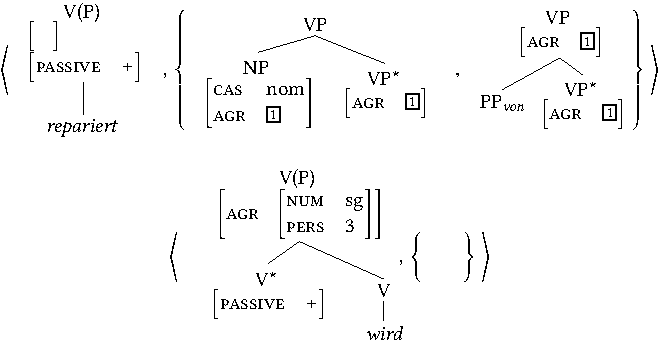
\includegraphics{graphics/abb722.pdf}
\caption{\label{fig-ttmctag-pass-1}Baumtupel für die Derivation der Passivkonstruktion in \ref{ex-ttmctag-pass}}
\end{figure} 
Das \isi{Hilfsverb} {\it wird} selegiert per {\sc passive}-Merkmal ein Passiv-Partizipium wie {\it repariert}, dessen Argumentbäume aus einer Nominativ-NP und einer \emph{von}-PP bestehen. In Baumtupeln für Perfekt-Partizipia\is{Perfekt} würde u.\,a.\ der Argumentbaum für \emph{von}-PPs fehlen. Die Subjekt-Verb-Kongruenz\is{Kongruenz} wird indirekt durchgesetzt: Die Kongruenzmerkmale im komplexen Merkmal {\sc agr(eement)} werden ausgehend vom Hilfsverb entlang der Verbprojektion  weitergereicht und von der Nominativ"=NP abgegriffen. Dagegen erfolgt die Nominativ-Kasusmarkierung lexikalisch, d.\,h.\ direkt im Baumtupel von {\it repariert}.

Schauen wir nun die Fernpassiv-Konstruktion in \ref{ex-ttmctag-pass-2} an:

\ex. \label{ex-ttmctag-pass-2} wenn der Kühlschrank von Peter zu reparieren versucht wird

Hier regiert das Passiv-Partizip {\it versucht} den 2.~Status des Verbs {\it zu reparieren}, dessen Objekt {\it der Kühlschrank} im Nominativ steht und nicht wie bei der Aktiv-Diathese in \ref{ex-ttmctag-fern-a} im Akkusativ. Die \emph{von}-PP {\it von Peter} realisiert eine \isi{semantische Rolle} sowohl von {\it versucht} als auch von {\it zu reparieren}, wird aber im Folgenden als Ergänzung des Passiv-Partizips behandelt. Es stellt sich dann die Frage, wie die Kasusvariabilität des Objekts des Status-2-Verbs modelliert werden soll. Zwei Modellierungsmöglichkeiten im Rahmen der TT-MCTAG bestehen: (i) Der Kasus\is{Kasusmarkierung} wird lexikalisch im Baumtupel von {\it zu reparieren} zugewiesen. Dann benötigt man zwei Arten von Baumtupeln, nämlich je eine für Akkusativ und Nominativ, die durch spezielle Merkmale (analog zum {\sc passive}-Merkmal bei Partizipia) unterschieden und selegierbar gemacht werden müssen. Oder (ii) der Kasus\is{Kasusmarkierung} wird mittels \isi{Merkmalsperkolation} von einem regierenden Verb zugewiesen. Das erspart zwar die Annahme spezieller Baumtupel-Paare für {\it zu reparieren}, macht aber einen Spezifizierung der Merkmalsperkolation nötig. Mir erscheint der zweite Modellierungsweg attraktiver, da eine Merkmalsperkolation in der syntaktischen Struktur unabhängig davon auch für die Modellierung der Subjekt-Verb-Kongruenz\is{Kongruenz} in Anhebungskonstruktionen\is{Anhebung} ratsam ist. 

Dieser zweite Ansatz wird in Abbildung~\ref{fig-ttmctag-fern-2} durchgespielt. 
\begin{figure}[t]
\centering
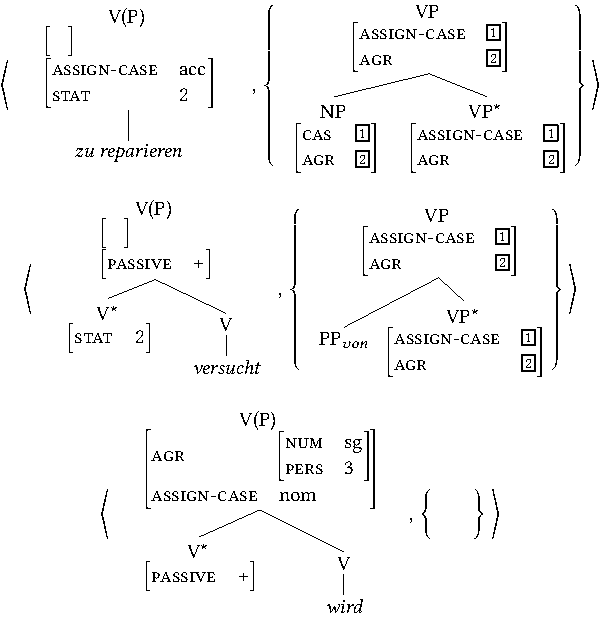
\includegraphics{graphics/abb723.pdf}
\caption{\label{fig-ttmctag-fern-2}Baumtupel für die Derivation des Fernpassivs in \ref{ex-ttmctag-fern-b}}
\end{figure}
Dort ist im NP-Blatt des Argumentbaums von {\it zu reparieren} das Kasusmerkmal\is{Kasus} ({\sc cas}) und das Kongruenzmerkmal\is{Kongruenz} ({\sc agr}) unterspezifiziert. Beide Merkmale sind jedoch mit Merkmalen auf der Verbprojektion verlinkt. Die Kasuszuweisung\is{Kasusmarkierung} erfolgt durch das Merkmal {\sc assign-case},\footnote{Das Merkmal {\sc assign-case} ist aus der XTAG-Grammatik\is{XTAG} übernommen und dient dort ebenfalls zur Kasusmarkierung valenzfremder NPs.} das in dem Kopfbaumwurzelknoten von {\it zu reparieren} einen Akkusativwert zugewiesen wird. Allerdings ist die Kasuszuweisung mit {\sc assign-case} nur im {\sc bottom}-Bereich spezifiziert und damit prinzipiell durch Adjunktion veränderbar. Das Passivhilfsverb\is{Hilfsverb} {\it wird} nützt diesen Umstand aus, unterbricht die Perkolation der Akkusativzuweisung (ebenso wie der Kopfbaum von {\it versucht}) und weist stattdessen per {\sc assign-case} den Nominlativkasus zu. Man beachte, dass das {\it wird}-Baumtupel mit {\sc assign-case} auch für die Derivation des einfachen Passiv in \ref{ex-ttmctag-pass} geeignet ist. %\ifdraft{\marginpar{Vgl.\ mit Reapes Lokalitätsdomänen \citep{Kathol:98}}} 

Die Verteilung von Kasusmarkierung und Valenzbindung auf zwei unterschiedliche Verben hat erfreuliche Konsequenzen für die Modellierung partieller Voranstellungen\is{Voranstellung!partielle} in Fernpassiv-Konstruktionen wie \ref{ex-ttmctag-pass-3}:

%\clearpage

\ex. \label{ex-ttmctag-pass-3} Der Wagen zu reparieren versucht wurde lange Zeit. \hfill \citep[(316-b)]{Meurers:99}

{\it Der Wagen} ist hier eine Ergänzung von {\it zu reparieren}, soll aber vom finiten Passivhilfsverb {\it wurde} seinen Kasus erhalten. Man kann daraus schlussfolgern, dass  für die Zugänglichkeit zu einem vorangestelltem Kohärenzfeld allein die \isi{Valenzbindung} (bzw.\ Valenzrahmenzugehörigkeit) ausschlaggebend ist.  {\it Der Wagen} kann also deshalb mit {\it zu reparieren versucht} vorangestellt werden, weil es sich dabei um eine \isi{Ergänzung} von {\it zu reparieren} handelt. Da die Node-Sharing-Lokalität\is{Node Sharing} auf Grundlage von Baumtupeln entschieden wird, die durch das Valenzprinzip\is{Wohlgeformtheitsprinzip!Valenzprinzip für TT-MCTAG} motiviert sein müssen, fällt eine Erfassung solcher Voranstellungsdaten wie in \ref{ex-ttmctag-pass-3} nicht schwer. Es muss den Baumtupeln in Abbildung~\ref{fig-ttmctag-fern-2} nur ein Baumtupel wie in Abbildung~\ref{fig-ttmctag-fern-3} hinzugefügt werden, das eine Voranstellung bewirkt und die gewünschte \isi{Merkmalsperkolation} in Gang setzt. 
\begin{figure}[t]
\centering
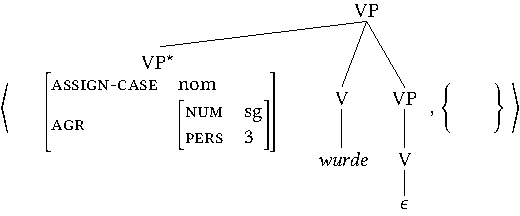
\includegraphics{graphics/abb724.pdf}
\caption{\label{fig-ttmctag-fern-3}Baumtupel für das voranstellende Passivhilfsverb {\it wurde}}
\end{figure}
\is{Passiv!Fern-|)}  

\is{Voranstellung!partielle|(}
Von der Modellierung passivischer Voranstellungdaten wie \ref{ex-ttmctag-pass-3} ist es schlie\ss lich nicht weit zur Modellierung von partiellen VP-Voranstellungen in aktivischen Sätzen. Auch hier kann, wie schon mehrfach erwähnt, ein \isi{Subjekt} in die Voranstellung einbezogen werden, falls das kasusmarkierende Verb nicht gleichzeitig in einer Valenzbeziehung zum Subjekt steht. Dies ist naturgemä\ss\ in Anhebungskonstruktionen\is{Anhebung} der Fall, also in Passivkonstruktionen (mit dem Passivhilfsverb als Anhebungsverb) oder in Konstruktionen wie \ref{ex-ttmctag-pass-4} mit dem Anhebungsverb {\it scheinen}:  

\ex. \label{ex-ttmctag-pass-4} 
\a. \label{ex-ttmctag-pass-4-a} Ein Au\ss enseiter zu gewinnen scheint hier eigentlich nie. \hfill \citep[(265)]{Meurers:99}
\b. \label{ex-ttmctag-pass-4-b} Ein Lehrling den Wagen zu reparieren scheint hier eigentlich nie.

Beim Vergleich von \ref{ex-ttmctag-pass-4-b} mit dem vorangestellten Fernpassiv in \ref{ex-ttmctag-pass-3} fällt zunächst auf, dass {\it zu reparieren} neben der Patiensrolle {\it den Wagen} auch die Agensrolle {\it ein Lehrling} realisiert. Da beide Rollen nicht zum Rollenbestand von {\it scheint} gehören, müssen sie im Baumtupel von {\it zu reparieren} repräsentiert sein. Das ist in Abbildung~\ref{fig-ttmctag-fern-4} auch der Fall.
\begin{figure}[t]
\centering
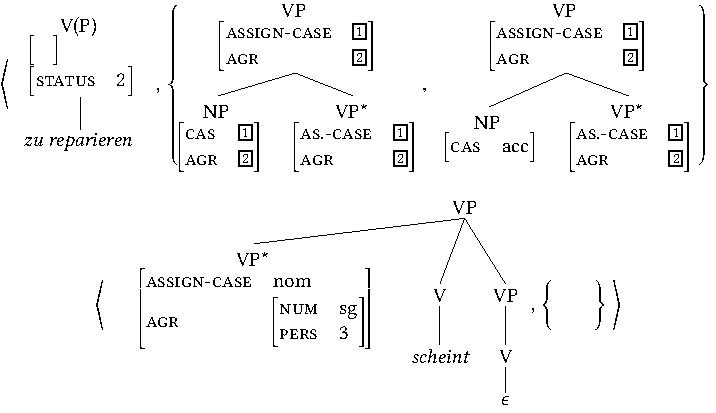
\includegraphics{graphics/abb725.pdf}
\caption{\label{fig-ttmctag-fern-4}Baumtupel für die partielle VP-Voranstellung in \ref{ex-ttmctag-pass-4-b}}
\end{figure}
Die Voranstellung des Subjekts\is{Subjekt} ist also deswegen möglich, weil es als Argumentbaum des vorangestellten Kopfes {\it zu reparieren} fungiert und diesem per Node-Sharing-Lokalität\is{Node Sharing} die Vorfeldphrase zugänglich ist.

Unzugänglich soll die Vorfeldphrase dagegen in den Fällen sein, wo das finite Verb das \isi{Subjekt} nicht anhebt, sondern qua Valenz direkt regiert. Eine Voranstellung wie in \ref{ex-ttmctag-pass-5} mit dem Kontrollverb\is{Kontrolle} {\it versuchen} an Stelle des Anhebungsverbs {\it scheinen} soll also verhindert werden:  

\ex. \label{ex-ttmctag-pass-5} *Ein Lehrling den Wagen zu reparieren versucht hier eigentlich nie.

Dass {\it ein Lehrling} als Ergänzung von {\it versucht} nicht in der Vorfeldphrase platziert werden kann, folgt in der TT-MCTAG-Modellierung direkt aus der Lokalitätsbeschränkung, die für die Verwendung eines Baumtupels gilt: Ein Kopfbaum kann nicht an seinen \isi{Argumentbaum} adjungieren, denn im Ableitungsbaum dominiert ein \isi{Kopfbaum} immer seine Argumentbäume.  Genau das umgekehrte Dominanzverhältnis wäre aber nötig, wenn \textit{versucht} den Elementarbaum von \textit{scheint} in Abbildung~\ref{fig-ttmctag-fern-4} ankern würde. Denn dann müsste der Subjekt-Argumentbaum im Fall einer Voranstellung unterhalb des Fu\ss knotens des Kopfbaums stehen (aufgrund der \isi{Vorfeldbündelung}) und damit im Ableitungsbaum den Kopfbaum dominieren.\is{Voranstellung!partielle|)}

So weit die Skizzierung der TT-MCTAG-Modellierung des Fernpassivs und der Subjekt-Voranstellung. Zusammenfassend kann man deren Strategie folgenderma\ss en charakterisieren: 
In Fällen der \isi{Anhebung} kann die \isi{Kasusmarkierung}, wie auch die Subjekt-Verb-Kongruenz\is{Kongruenz}, mittels \isi{Merkmalsperkolation} in der abgeleiteten syntaktischen Struktur erfolgen, während die Lokalitätsbeschränkungen generell von der valenztheoretisch fundierten Gestalt lexikalischer Baumtupel bestimmt werden. Als Folge dieser Modellierungsstrategie muss eine systematische Ambiguität der Status-2-Verben in Kauf genommen werden, will man nicht auf leere PRO-NPs\is{PRO} zurückgreifen. 

In dieser Hinsicht gibt es naturgemä\ss\ gewisse Ähnlichkeiten zu Reapes HPSG-Ansatz\is{Head-driven Phrase Structure Grammar (HPSG)} mit Linearisierungsdomänen\is{Linearisierungsdomäne}, der ja ebenfalls eine direkte diskontinuierliche Valenzrealisierung durchführt. Auch dort kann Fernpassiv und Anhebung nur indirekt über dazu bestimmte syntaktische Merkmale kontrolliert werden (\citealt[Abschnitt~5.1]{Kathol:98}; \citealt[Abschnitt~21.1]{Mueller:99}; \citealt[Abschnitt~8.6]{Kathol:00}). Im TAG-Framework, wo die \isi{Valenzvereinigung} nicht zur Verfügung steht, ist das kein ungewöhnlicher Weg -- anders als vielleicht im HPSG"=Framework.\footnote{\citet[279]{Mueller:07} kritisiert, dass diese Lösung "`ad hoc"' sei. Doch selbst in einem HPSG-Valenz\-vereinigungs\-ansatz wie dem von \cite{Meurers:99} können Kasus und Kongruenz nicht immer ohne Weiteres direkt festgelegt werden. Üblicherweise werden dort Rektionsbeziehungen\is{Rektion} anhand der {\sc subcat}-Liste spezifiziert und die {\sc subcat}-Liste dann entlang der Kopfprojektion entleert. Da aber das Subjekt in einer vorangestellten VP eingebettet sein kann (siehe \ref{ex-ttmctag-pass-4}), muss Meurers die Existenz sogenannter Geister ("`spirits"') auf der {\sc subcat}-Liste (bzw.\ im {\sc subj}-Merkmal) stipulieren, damit die Kasus- und Kongruenzmerkmale des eingebetteten Subjekts für das Anhebungsverb noch sichtbar sind.}   



\section{Die Grenzen von TT-MCTAG} \label{sec-ttmctag-grenzen}

Zwischen den Analysebeispielen in Abschnitt \ref{sec-ttmctag-beispiele} fanden sich bereits Hinweise auf die derivationellen Unzulänglichkeiten des hier dargestellten TT"=MCTAG"=Ansatzes. In diesem Abschnitt werden wir diesen Unzulänglichkeiten auf den Grund gehen, d.\,h.\ ihre Voraussetzungen untersuchen und Anpassungsmöglichkeiten erkunden. Abschlie\ss end möchte ich einen Vergleich mit einem analogen V-TAG-Ansatz anstellen.  

\subsection{Grenzziehung durch drei Einschränkungen}

Die Gestalt der Elementarstrukturen des in dieser Arbeit vorgestellten TT"=MCTAG"=Ansatzes und ihre Verknüpfung sind einer Reihe von Einschränkungen unterworfen, die linguistisch oder komplexitätstheoretisch motiviert sind. Im Zusammenhang mit den Unzulänglichkeiten bei der Erfassung von Kohärenzphänomenen ist der Geltungsbereich der folgenden Einschränkungen wesentlich: (i) das Valenzprinzip, (ii) die Annahme von rechtsverzweigenden Phrasenstrukturen und (iii) die Node-Sharing-Lokalität bei der Verwendung von Tupeln. 

%\subsubsection*{Valenzprinzip}
\is{Wohlgeformtheitsprinzip!Valenzprinzip für TT-MCTAG}

Das Valenzprinzip für TT-MCTAG wurde oben in \ref{ex-valenzprinzip-mctag} (S.\,\pageref{ex-valenzprinzip-mctag}) formuliert. In \ref{ex-ttmctag-valenz} wird es wiederholt:

\ex. \label{ex-ttmctag-valenz}{\bf Valenzprinzip (für TT-MCTAG)} \\ 
Baumtupel entsprechen genau einem Valenzrahmen, wobei gilt:
\a. Der lexikalische Anker im Kopfbaum ist der Valenzträger.
\b. Es besteht ein bijektives Abbildungsverhältnis zwischen Valenzrollen einerseits und Substitutionsknoten und dem Kopfbaumfu\ss knoten andererseits.

%\subsubsection*{Rechtsverzweigende Phrasenstrukturen}
\is{Phrasenstruktur!rechtsverzweigende}

Im Einklang mit Phrasenstrukturkonventionen für die Satzsyntax nehme ich für V1- und V2-Sätze eine rechtsverzweigende Phrasenstruktur wie in Abbildung~\ref{fig-ttmctag-ps-2} an (modulo ternär verzweigende Vorfeldknoten bei partieller Voranstellung).
\begin{figure}[t]
\centering
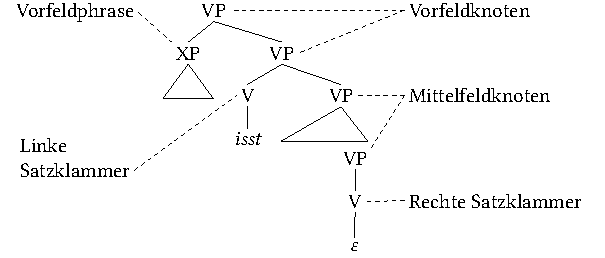
\includegraphics{graphics/abb726.pdf}
\caption{\label{fig-ttmctag-ps-2}Phrasenstrukturschema eines V2-Satzes (Wiederholung von Abbildung~\ref{fig-ttmctag-ps-1})}
\end{figure} 
Darin dominieren die Vorfeldknoten den Knoten der linken Satzklammer und die Mittelfeldknoten, und letzterer wiederum den Knoten der rechten Satzklammer. Daneben ist das Vorfeld unter einer Phrase gebündelt\is{Vorfeldbündelung}. Die Bedeutung dieser Phrasenstruktur für die TT-MCTAG-Modellierung wird im Phrasenstrukturprinzip\is{Wohlgeformtheitsprinzip!Phrasenstrukturprinzip} festgehalten (siehe auch S.\,\pageref{ex-psprinzip}):

\ex. {\bf Phrasenstrukturprinzip (für V2-Sätze):}
Der abgeleitete Baum enthält nur die vollständigen Projektionen der lexikalischen Anker und ist eine Instanz des Phrasenstrukturschemas in Abbildung~\ref{fig-ttmctag-ps-2}.


%\subsubsection*{Node-Sharing-Lokalität}
\is{Node Sharing|(}

Die Node-Sharing-Lokalität als Beschränkung der Argumentbaumverwendung ist ein Bestandteil des TT-MCTAG-Formalismus (siehe Definition \ref{def-ttmctag-ab}, S.\,\pageref{def-ttmctag-ab}). Sie besagt in einfachen Worten: Ein \isi{Argumentbaum} $\beta_i$ adjungiert Node-Sharing-lokal am \isi{Kopfbaum} $\gamma$, wenn $\beta_i$ entweder direkt an $\gamma$ adjungiert oder indirekt an den Wurzelknoten eines anderen Hilfsbaums, der an $\gamma$ Node-Sharing-lokal adjungiert. Bei einer \isi{Adjunktion} wird also nur der Wurzelknoten des adjungierenden Hilfsbaums geteilt.  
%
Anders als die Formulierung des Valenzprinzips und die Wahl einer Phrasenstruktur ist die Wahl der Node-Sharing-Lokalität komplexitätstheoretisch begründet: Die formale Ausdrucksstärke\is{TT-MCTAG!Ausdrucksstärke} des TT-MCTAG-Formalismus soll nur so gro\ss\ sein, wie es die Modellierung der strukturellen und derivationellen Eigenschaften eines Satzes verlangt und dabei die MCS-Kriterien\is{schwache Kontextsensitivität} erfüllen. Strukturelle und derivationelle Eigenschaften sind wiederum grammatiktheoretische Grö\ss en. Verallgemeinert lässt sich also sagen, dass sich die Frage der notwendigen Ausdrucksstärke nicht losgelöst von grammatiktheoretischen Rahmenbedingungen beantworten lässt. Im nächsten Abschnitt werde ich die Wechselwirkung dieser Faktoren anhand dreier ausgewählter Grenzfälle veranschaulichen. 
\is{Node Sharing|)}


\subsection{Jenseits der Grenzen}

Im Geltungsbereich von Valenzprinzip, Phrasenstrukturprinzip (in der oben dargelegten Formulierung) und Node-Sharing-Lokalität können gewisse Konstruktionstypen nicht durch eine TT-MCTAG erfasst werden. Es sind allerdings Anpassungen dieser Einschränkungen denkbar, die zu einer größeren derivationellen Mächtigkeit\is{derivationelle Mächtigkeit} führen und damit den Abdeckungsbereich der TT-MCTAG vergrößern. Ich werde hier drei Grenzfälle vorstellen, die sich letztlich in Art und Umfang der nötigen Anpassung unterscheiden, die zu ihrer Erfassung notwendig ist. 
%
Gemein ist diesen Grenzfällen die Existenz eines echt-dominierten Mittelfeldknotens, also das Vorliegen einer V1/V2-Satzstellung\is{Satz!V1-}\is{Satz!V2-},\footnote{Da das Dominanzverhältnis reflexiv ist, unterscheide ich zwischen Dominanz und \textsc{echter Dominanz}. Letztere besteht nur zwischen zwei Knoten $v_1, v_2 \in V$ für einen Baum $D = (V,E)$ mit reflexiv transitiver Dominanzrelation $\Rightarrow^*$, falls $v_1 \Rightarrow^* v_2$ und $v_1 \neq v_2$.} und die Adjunktion des Argumentbaums eines infiniten Verbs am Mittelfeldknoten. Die Position des infiniten Verbs ist dagegen in den Grenzfälle variabel und daher Bezugspunkt ihrer Unterscheidung. 

\subsubsection*{Erster Grenzfall}

Als ersten Grenzfall betrachte ich die TT-MCTAG-Modellierung von Satz \ref{ex-ttmctag-grenzen-1}, in dem das Infinitum {\it zu reparieren} im Schlussfeld steht und dessen Ergänzung {\it ihn} Teil des Mittelfelds ist:\is{kohärente Konstruktion!Intraposition}\footnote{Die TT-MCTAG-Modellierung von \ref{ex-ttmctag-grenzen-1} ist hier auch stellvertretend für die TT-MCTAG-Modellierung von Fällen der 3.~Konstruktion\is{kohärente Konstruktion!3.~Konstruktion}, bei der das infinite Verb extraponiert ist und seine Ergänzung im Mittelfeld erscheint (siehe \ref{ex-ttmctag-extra2} auf Seite~\pageref{ex-ttmctag-extra2}).} 

\ex. Heute versucht ihn Peter zu reparieren. \label{ex-ttmctag-grenzen-1}

Für diesen Satz wird entsprechend des Phrasenstrukturprinzips\is{Wohlgeformtheitsprinzip!Phrasenstrukturprinzip} der abgeleitete Baum in Abbildung~\ref{fig-ttmctag-grenzen-1} angenommen. Die gestrichelte Kante und das unübliche Knotenlabel V$|$VP weisen darauf hin, dass hier zwei Analyseansätze sinnvoll sind. 
\begin{figure}[t]
\centering
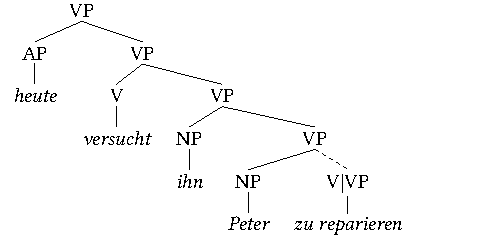
\includegraphics{graphics/abb727.pdf}
\caption{\label{fig-ttmctag-grenzen-1}Phrasenstruktur für \ref{ex-ttmctag-grenzen-1}. Die gestrichelte Kante und das Kantenlabel VP|V deuten die zwei unterschiedliche Ableitungsmöglichkeiten in Abbildung~\ref{fig-ttmctag-grenzen-2-b} an.}
\end{figure} 
Sie schlagen sich in Form zweier unterschiedlicher Kopfbäume für das {\it versucht}-Tupel nieder, dargestellt in Abbildung~\ref{fig-ttmctag-grenzen-2}, in denen ein Mittelfeldknoten vorhanden sein kann oder nicht. Das {\it zu reparieren}-Tupel ist dagegen bereits aus den den Analysebeispielen in Abschnitt~\ref{sec-ttmctag-beispiele} bekannt.\footnote{Gleichwohl könnte man den Mittelfeldknoten auch im Kopfbaum von {\it zu reparieren} unterbringen. Das ändert jedoch nichts an der spezifischen Unzulänglichkeit des Ansatzes, von der hier die Rede ist.}     
\begin{figure}[t]
\centering
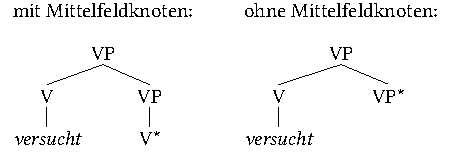
\includegraphics{graphics/abb728.pdf}
\caption{\label{fig-ttmctag-grenzen-2}Zwei alternative Kopfbäume für {\it versucht}, die zu den zwei Ableitungsmöglichkeiten in Abbildung~\ref{fig-ttmctag-grenzen-2-b} und dem abgeleiteten Baum in Abbildung~\ref{fig-ttmctag-grenzen-1} führen}
\end{figure} 
Beide {\it versucht}-Kopfbäume können jedoch nicht zur Generierung der Struktur in Abbildung~\ref{fig-ttmctag-grenzen-1} führen: Inkorporiert der {\it versucht}-Kopfbaum einen Mittelfeldknoten, dann ist es zwar möglich, dessen Argumentbäume im Mittelfeld zu platzieren, aber der Argumentbaum von {\it zu reparieren} hat aufgrund der Node-Sharing-Lokalität\is{Node Sharing} keinen Zugang, da der Mittelfeldknoten nicht der Wurzelknoten des {\it versucht}-Kopfbaums ist; im anderen Fall ohne Mittelfeldknoten kann zwar der Argumentbaum von {\it zu reparieren} im Mittelfeld platziert werden, dafür scheitert nun eine dortige Adjunktion des {\it versucht}-Argumentbaums. Das Dilemma wird auch mit Blick auf die Ableitungsbäume in Abbildung~\ref{fig-ttmctag-grenzen-2-b} deutlich: Entweder der Pfad zwischen {\tt zu\_reparieren} und {\tt NP$_{acc}$} enthält eine Adjunktion an einer Adresse unterhalb des Wurzelknotens (hier {\sc a.2}), oder der Argumentbaum {\tt NP$_{nom}$} dominiert den Kopfbaum {\tt versucht}, was ebenfalls durch die Node-Sharing-Lokalität verboten ist. 
\begin{figure}[t]
\centering
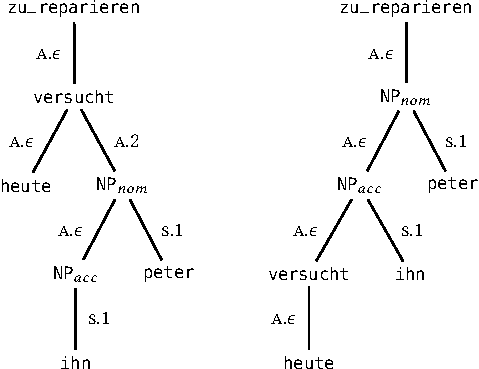
\includegraphics{graphics/abb729.pdf}
\caption{\label{fig-ttmctag-grenzen-2-b}Ableitungsbaum mit {\it versucht}-Kopfbaum mit Mittelfeldknoten (links) und Ableitungsbaum mit {\it versucht}-Kopfbaum ohne Mittelfeldknoten (rechts)}
\end{figure} 

Um Instanzen dieses Grenzfalltyps dennoch zu generieren, gibt es zwei Anpassungsmöglichkeiten bei den Rahmenbedingungen, nämlich (i) die Erweiterung der Node-Sharing-Lokalität\is{Node Sharing} oder (ii) die Lockerung des Valenzprinzips\is{Wohlgeformtheitsprinzip!Valenzprinzip für TT-MCTAG}. Eine minimale Erweiterung der Node-Sharing-Lokalität könnte etwa die Knoten auf dem Pfad zwischen Wurzel- und Fu\ss knoten in das Sharing-Verhältnis einbeziehen.\footnote{Könnte man am Fu\ss knoten adjungieren, dann lie\ss e sich womöglich die Erweiterung des Node Sharings auf die Einbeziehung des Fu\ss knotens beschränken. Da die Spines aber in den betrachteten Elementarbäumen meist nur aus zwei Knoten bestehen, dem Wurzelknoten und dem Fu\ss knoten, ist das \isi{Spine Sharing} sogar in vielen Fällen sparsamer hinsichtlich der Stipulierung geteilter Knoten.} Im Geltungsbereich dieser sogenannte \textsc{Spine-Sharing-Lokalität}\is{Spine Sharing} kann der {\it versucht}-Elementarbaum mit Mittelfeldknoten in Abbildung~\ref{fig-ttmctag-grenzen-2} zur Generierung des Ableitungsbaums in Abbildung~\ref{fig-ttmctag-grenzen-1} verwendet werden, da nun der Mittelfeldknoten für den Argumentbaum von {\it zu reparieren} zugänglich ist. Alternativ ist jedoch auch eine Lockerung des Valenzprinzips\is{Wohlgeformtheitsprinzip!Valenzprinzip für TT-MCTAG} denkbar, so dass auch Tupel zulässig sind, deren Kopfbäume\is{Kopfbaum} nicht durch den \isi{Valenzträger} lexikalisiert sind. Das {\it versucht}-Tupel könnte beispielsweise dann die Gestalt in Abbildung~\ref{fig-ttmctag-grenzen-1-2} annehmen, in der der Vorfeldknoten und die linke Satzklammer (mit dem Finitum) vom Mittelfeldknoten und der rechte Satzklammer getrennt worden ist. Der Mittelfeldknoten ist dadurch sowohl für die Argumentbäume des {\it versucht}-Tupels als auch für den Argumentbaum des {\it zu reparieren}-Tupels zugänglich. 

\begin{figure}[t]
\centering
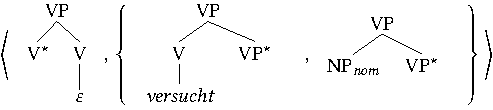
\includegraphics{graphics/abb730.pdf}
\caption{\label{fig-ttmctag-grenzen-1-2}Baumtupel für {\it versucht} ohne Valenzträger im Kopfbaum}
\end{figure}   


\subsubsection*{Zweiter Grenzfall}

Der zweite Grenzfall ist die partielle Voranstellung\is{Voranstellung!partielle} infiniter Verben, d.\,h.\ das infinite Verb tritt im Vorfeld auf, seine Ergänzung aber im Mittelfeld. Ein Beispiel dafür befindet sich in \ref{ex-ttmctag-grenzen-2}:   

\ex. Zu reparieren versucht ihn Peter. \label{ex-ttmctag-grenzen-2}

Gemä\ss\ des Phrasenstrukturprinzips\is{Wohlgeformtheitsprinzip!Phrasenstrukturprinzip} erwarten wir für \ref{ex-ttmctag-grenzen-2} einen abgeleiteten Baum wie in Abbildung~\ref{fig-ttmctag-grenzen-3}. Derivationell verantwortlich kann dafür der Elementarbaum des Finitums {\it versucht}, abgebildet in Abbildung~\ref{fig-ttmctag-grenzen-4}, gemacht werden. Wieder ist also der Mittelfeldknoten für den Argumentbaum von {\it zu reparieren} nach Ma\ss gabe der Node-Sharing-Lokalität\is{Node Sharing} unzugänglich und damit der abgeleitete Baum nicht generierbar.
 
\begin{figure}[t]
\centering
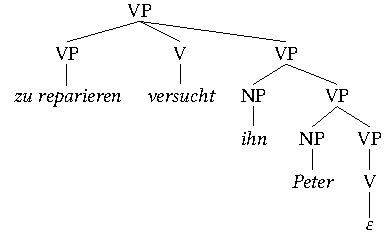
\includegraphics{graphics/abb731.pdf}
\caption{\label{fig-ttmctag-grenzen-3}Phrasenstruktur für die partielle Voranstellung in \ref{ex-ttmctag-grenzen-2}}
\end{figure} 
%%%%%%%%%%%%%%%%%%%%%%%%%%%%%%%%%%%%%%%%%%
\begin{figure}[t]
\centering
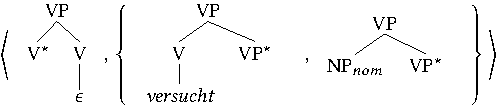
\includegraphics{graphics/abb732.pdf}
\caption{\label{fig-ttmctag-grenzen-4}{\it versucht}-Kopfbaum für die Ableitung der partiellen Voranstellung in \ref{ex-ttmctag-grenzen-2}, wobei eine Tree-Sharing-Lokalität benötigt wird}
\end{figure} 

Für die Erfassung des zweiten Grenzfalls sind die folgenden Anpassungsoptionen erfolgversprechend: (i) Erweiterung der Node-Sharing-Lokalität\is{Node Sharing}, (ii) Lockerung des Valenzprinzips\is{Wohlgeformtheitsprinzip!Valenzprinzip für TT-MCTAG} und (iii) Gebrauch einer linksverzweigenden Phrasenstruktur\is{Phrasenstruktur!linksverzweigende}. Anders als beim ersten Grenzfall erweist sich hier jedoch eine Spine-Sharing-Lokalität\is{Spine Sharing} als unzureichend, da der Mittelfeldknoten bei der Voranstellung nicht auf dem Pfad zwischen Wurzel- und Fu\ss knoten liegt. Um den Mittelfeldknoten erreichbar zu machen, bietet es sich an, die Spine-Sharing-Lokalität zu einer \textsc{Tree-Sharing-Lokalität}\is{Tree Sharing} auszuweiten, d.\,h.\ alle Knoten eines adjungierenden Hilfsbaums in das Sharing-Verhältnis einzubeziehen. Damit könnte der {\it versucht}-Kopfbaum in Abbildung~\ref{fig-ttmctag-grenzen-4} beibehalten werden. Allerdings reicht auch die Spine-Sharing-Lokalität aus, wenn stattdessen die Kopfbäume in Abbildung \ref{fig-ttmctag-grenzen-ii-3} verwendet werden. Hier geht die Voranstellung vom infiniten Verb aus, nicht vom Finitum, welches in der Standardform für V1/V2-Satztypen realisiert wird (vgl.\ Abbildung~\ref{fig-ttmctag-koh1}, S.\,\pageref{fig-ttmctag-koh1}).  

\begin{figure}[t]
\centering
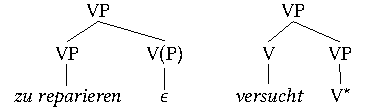
\includegraphics{graphics/abb733.pdf}
\caption{\label{fig-ttmctag-grenzen-ii-3}Alternative Kopfbäume, die unter Spine-Sharing-Lokalität zur Ableitung von \ref{ex-ttmctag-grenzen-2} eingesetzt werden können. Der \textit{versucht}-Baum muss dafür an den V(P)-Knoten des \textit{zu reparieren}-Baums adjungieren.}
\end{figure}

Alternativ, d.\,h.\ unter Beibehaltung der Node-Sharing-Lokalität, könnte man wiederum eine Lockerung des Valenzprinzips\is{Wohlgeformtheitsprinzip!Valenzprinzip für TT-MCTAG} vornehmen und die Gestalt der Tupel verändern. {\it zu reparieren} könnte dann mithilfe das Tupels in Abbildung~\ref{fig-ttmctag-grenzen-ii-4} modelliert werden, das im Zusammenspiel mit dem {\it versucht}-Tupel in Abbildung~\ref{fig-ttmctag-grenzen-1-2} die wesentlichen Struktureigenschaften des abgeleiteten Baums aus Abbildung~\ref{fig-ttmctag-grenzen-3} zu erzeugen und dem Phrasenstrukturprinzip\is{Wohlgeformtheitsprinzip!Phrasenstrukturprinzip} zu genügen vermag. Ein gravierendes Defizit dieser Lösung ist jedoch, dass die Voranstellung allein das infinite Verb betrifft. Ein Satz wie \ref{ex-ttmctag-grenzen-ii-2} kann damit nicht abgeleitet werden, ohne die \isi{Vorfeldbündelung} einzubüßen:

\ex. Ihn zu reparieren versuchte Peter nicht. \label{ex-ttmctag-grenzen-ii-2}  

\begin{figure}[t]
\centering
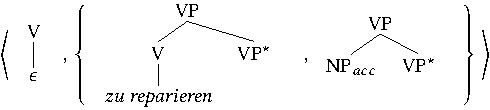
\includegraphics{graphics/abb734.pdf}
\caption{\label{fig-ttmctag-grenzen-ii-4}Baumtupel für {\it zu reparieren} ohne Valenzträger im Kopfbaum}
\end{figure}

Eine weitere Anpassungsoption betrifft die Orientierung der Phrasenstruktur. Man könnte nämlich auch eine linksverzweigende Struktur\is{Phrasenstruktur!linksverzweigende} wie in Abbildung~\ref{fig-ttmctag-ii-5} erzeugen.\footnote{\cite{Crysmann:03} schlägt im Rahmen der HPSG\is{Head-driven Phrase Structure Grammar (HPSG)} solche linksverzweigenden Strukturen\is{Phrasenstruktur!linksverzweigende} vor, um leere verbale Kategorien bei Verbbewegungsanalysen\is{Bewegung} zu verhindern und das Parsen mit HPSG-Grammatiken effizienter zu machen. Das gilt allerdings nur für V1\is{Satz!V1-}, da bei V2 das Vorfeld über Bewegung aus dem Mittelfeld besetzt wird und daher strukturell höher steht als die linke Satzklammer und das Mittelfeld. Siehe \cite{Mueller:05} für eine Erwiderung. Linksverzweigende HPSG-Analysen für alle Satzarten schlägt \cite{Haugereid:09} für das Englische und Norwegische vor. Nicht unerwähnt bleiben darf an dieser Stelle der Ansatz der Left-Associative Grammar \citep{Hausser:89}, der ausschließlich linksverzweigende Strukturen zulässt.}
\begin{figure}[t]
\centering
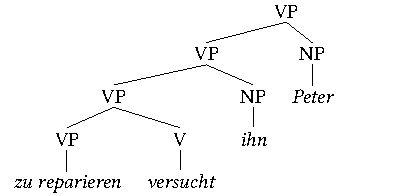
\includegraphics{graphics/abb735.pdf}
\caption{\label{fig-ttmctag-ii-5}Linksverzweigende Phrasenstruktur für die partielle Voranstellung in \ref{ex-ttmctag-grenzen-2} }
\end{figure}
Dementsprechend müssten die Tupel linksverzweigende Argumentbäume enthalten. Zwar widerspricht das Resultat den Sehgewohnheiten, aber ein Abweichen von der Node-Sharing-Lokalität und der strikten Form des Valenzprinzips lie\ss e sich dadurch umgehen. Unattraktiv hieran ist jedoch der eng begrenzte Nutzen dieser Anpassung, da für andere Konstruktionen wiederum eine rechtsverzweigende Struktur\is{Phrasenstruktur!rechtsverzweigende} vorteilhafter ist. Dazu mehr in Abschnitt~\ref{sec-ttmctag-grenzen-anpassung}. Zudem lässt sich auch bei einer linksverzweigenden Struktur\is{Phrasenstruktur!linksverzweigende} nicht immer vermeiden, dass eine Spine-Sharing-Lokalität\is{Spine Sharing} notwendig ist. Erstreckt sich das Finitum über beide Satzklammern wie in \ref{ex-ttmctag-grenzen-ii-3}, mit einem abtrennbaren Verbzusatz\is{abtrennbarer Verbzusatz} in der rechten Satzklammer, dann existiert wieder ein echt-dominierter Mittelfeldknoten:   

\ex. Zu reparieren fing ihn Peter an. \label{ex-ttmctag-grenzen-ii-3}  


\subsubsection*{Dritter Grenzfall}

Der dritte Grenzfall ist in gewisser Hinsicht der schwierigste der drei Grenzfälle. Dazu zählt beispielsweise die mehrfach partielle Voranstellung\is{Voranstellung!partielle} in \ref{ex-ttmctag-grenzen-iii-1}: 

\ex. Zu reparieren versprochen hat ihm das Peter. \label{ex-ttmctag-grenzen-iii-1}

Im Unterschied zur einfachen partiellen Voranstellung beim zweiten Grenzfall besteht das Vorfeld hier aus zwei infiniten Verben {\it zu reparieren} und {\it versprochen}, zwischen denen ein Rektionsverhältnis besteht und die jeweils eine Ergänzung, {\it das} bzw.\ {\it ihm}, im Mittelfeld regieren. Der abgeleitete Baum für \ref{ex-ttmctag-grenzen-iii-1} sollte so aussehen wie in Abbildung~\ref{fig-ttmctag-grenzen-iii}. 
\begin{figure}[t]
\centering
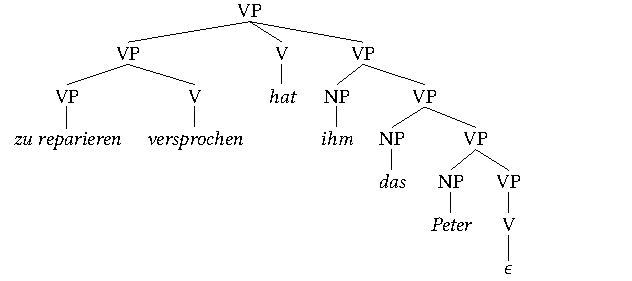
\includegraphics{graphics/abb736.pdf}
\caption{\label{fig-ttmctag-grenzen-iii}Phrasenstruktur der mehrfach partiellen Voranstellung in \ref{ex-ttmctag-grenzen-iii-1} mit Vor\-feld\-bündelung}
\end{figure}
Dessen Phrasenstruktur\is{Phrasenstruktur!rechtsverzweigende} ist also nicht nur rechtsverzweigend, sondern das Vorfeld ist unter einem VP-Knoten gebündelt\is{Vorfeldbündelung}, der nicht das Mittelfeld dominiert. Dies entspricht der Regel, dass das Vorfeld von maximal einer Konstituente besetzt werden kann (siehe Abschnitt \ref{sec-feldermodell}).    

Wünschenswert wäre die Verwendung der Kopfbäume in Abbildung~\ref{fig-ttmctag-grenzen-iii-2}, die oben bereits zum Einsatz kamen. Wie schon bei der einfachen partiellen Voranstellung ist dies aber nur unter einer Tree-Sharing-Lokalität\is{Tree Sharing} möglich, denn der Mittelfeldknoten liegt noch nicht einmal auf dem Pfad zwischen Wurzel- und Fu\ss knoten von {\it hat} oder {\it versprochen}. Spine-Sharing\is{Spine Sharing} allein ermöglicht also nicht die Adjunktion der Argumentbäume der vorangestellten Verbköpfe am Mittelfeldknoten.
\begin{figure}[t]
\centering
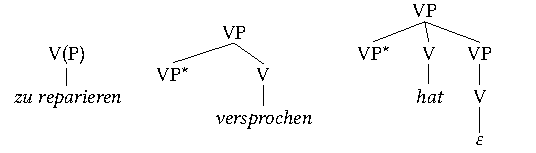
\includegraphics{graphics/abb737.pdf}
\caption{\label{fig-ttmctag-grenzen-iii-2}Kopfbäume für die Generierung der Phrasenstruktur in Abbildung \ref{fig-ttmctag-grenzen-iii} unter Tree-Sharing-Lokalität}
\end{figure}
Eine Beschränkung auf die Spine-Sharing-Lokalität (geschweige denn auf eine Node-Sharing-Lokalität) scheint selbst dann nicht möglich, wenn die Kopfbaumvarianten in Abbildung~\ref{fig-ttmctag-grenzen-iii-3} in die TT"=MCTAG"=Modellierung eingebracht werden. Diese Eigenschaft unterscheidet die mehrfache partielle Voranstellung von der einfach partiellen Voranstellung, bei der sich Kopfbäume wie in Abbildung~\ref{fig-ttmctag-grenzen-iii-3} dazu eignen, die Tree-Sharing-Lokalität\is{Tree Sharing} auf eine Spine-Sharing-Lokalität\is{Spine Sharing} zurückzuführen. Auch die Lockerung des Valenzprinzips\is{Wohlgeformtheitsprinzip!Valenzprinzip für TT-MCTAG} stellt keine Alternative zur Tree-Sharing-Lokalität dar. 
\begin{figure}[t]
\centering
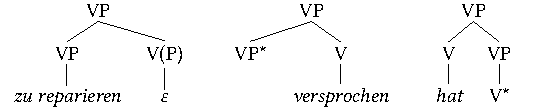
\includegraphics{graphics/abb738.pdf}
\caption{\label{fig-ttmctag-grenzen-iii-3}Alternative Kopfbäume für die Generierung der Phrasenstruktur in Abbildung \ref{fig-ttmctag-grenzen-iii}, die ebefalls nur unter Tree-Sharing-Lokalität verwendbar sind}
\end{figure}
 

Gibt man die Bündelung des Vorfelds\is{Vorfeldbündelung} auf und geht stattdessen von einer rechtsverzweigenden Strukur\is{Phrasenstruktur!rechtsverzweigende} wie in Abbildung~\ref{fig-ttmctag-grenzen-iii-4} aus, bei der die VP"=Projektion der linken Satzklammer bei jedem vorangestelltem Verb fortgesetzt wird, dann ergeben sich neue Spielräume. 
\begin{figure}[t]
\centering
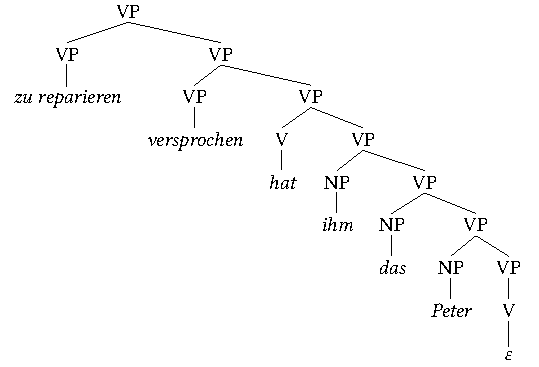
\includegraphics{graphics/abb739.pdf}
\caption{\label{fig-ttmctag-grenzen-iii-4}Phrasenstruktur der mehrfach partiellen Voranstellung in \ref{ex-ttmctag-grenzen-iii-1} ohne Vor\-feld\-bündelung}
\end{figure} 
Nun steht eine TT"=MCTAG"=Modellierung anhand der Kopfbäume in Abbildung~\ref{fig-ttmctag-grenzen-iii-5} zur Verfügung, der eine Spine"=Sharing"=Lokalität\is{Spine Sharing} genügt. Nimmt man zusätzlich noch eine Lockerung des Valenzprinzips\is{Wohlgeformtheitsprinzip!Valenzprinzip für TT-MCTAG} vor, reicht gar \isi{Node Sharing} aus. 
\begin{figure}[t]
\centering
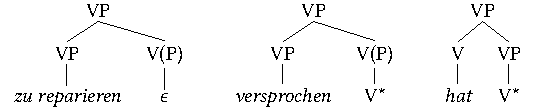
\includegraphics{graphics/abb740.pdf}
\caption{\label{fig-ttmctag-grenzen-iii-5}Kopfbäume für die Generierung der Phrasenstruktur ohne Vorfeldbündelung in Abbildung \ref{fig-ttmctag-grenzen-iii-4}, bei der die Spine-Sharing-Lokalität ausreicht}
\end{figure}
Alternativ kann man sich auf die Node-Sharing-Lokalität beschränken, wenn eine linksverzweigende Struktur\is{Phrasenstruktur!linksverzweigende} des Mittelfelds vorliegt. Hier bestehen also keine grundsätzlichen Unterschiede zwischen der mehrfach partiellen Voranstellung und der einfach partiellen Voranstellung\is{Voranstellung!partielle}. Dies schlie\ss t auch die Eigenschaft ein, eine Spine-Sharing-Lokalität zu erfordern, falls das Finitum einen abtrennbaren Verbzusatz\is{abtrennbarer Verbzusatz} in der rechten Satzklammer enthält.




\subsection{Anpassungsmöglichkeiten im Detail} \label{sec-ttmctag-grenzen-anpassung}

Die Ergebnisse des letzten Abschnitts sind in Tabelle~\ref{tab-ttmctag-grenzen-anpassung-1} zusammengefasst. Sie zeigt, durch welche Anpassungen am vorliegenden TT-MCTAG-Ansatz die betrachteten Grenzfälle modelliert werden können. In diesem Abschnitt werde ich die Anpassungsmöglichkeiten (Erweiterung der Sharing-Lokalität, Valenzprinzip und Phrasenstrukturpinzip) genauer betrachten und auf ihre grammatiktheoretischen und komplexitätstheoretischen Implikationen hin untersuchen. 

\begin{table}[ht]
\begin{center}

\begin{tabular}{l|ccc}
 & 1. GF & 2. GF & 3. GF \\
\hline
%Node-Sharing & - & - & - \\
Spine-Sharing & + & $-$/+ & $-$ \\ 
Tree-Sharing & + & + & + \\
abgeschw. Valenzprinzip & + & + & $-$ \\
linksverzweigende PS & $-$ & + & +  
\end{tabular}

\end{center}
\caption{\label{tab-ttmctag-grenzen-anpassung-1}Überblick über die Anpassungsmöglichkeiten und deren Auswirkungen auf die Modellierbarkeit der Grenzfälle}
\end{table}



\subsubsection*{Valenzprinzip}\is{Wohlgeformtheitsprinzip!Valenzprinzip für TT-MCTAG|(}

Die Anpassung des Valenzprinzips für TT-MCTAG, ausgehend von der Formulierung in \ref{ex-ttmctag-valenz}, war beim ersten und zweiten Grenzfall erfolgreich. Dabei bestand die Anpassung in einer Abschwächung, nämlich dass der \isi{Kopfbaum} nicht mehr vom \isi{Valenzträger} geankert werden muss. Statt \ref{ex-ttmctag-valenz} gilt also das ab\-ge\-schwäch\-te Valenzprinzip in \ref{ex-ttmctag-grenzen-anpassung-2}:

\ex. {\bf Abgeschwächtes Valenzprinzip (für TT-MCTAG):}\label{ex-ttmctag-grenzen-anpassung-2}\\
Baumtupel entsprechen genau einem Valenzrahmen, wobei gilt:
\a. Der Valenzträger lexikalisiert mindestens einen Elementarbaum des Baumtupels.
\b. Es besteht ein bijektives Abbildungsverhältnis zwischen Valenzrollen einerseits und Substitutionsknoten in der Argumentbaummenge bzw.\ Substitutionsknoten und Fu\ss knoten im Kopfbaum andererseits.

Die Folge ist, dass die Differenzierung von Valenzträger und Valenzrolle nunmehr alleine anhand der Lexikalisierung sichtbar ist. Das intuitive Verständnis eines Baumtupel, das sich in den Bezeichnungen "`Kopfbaum"' und "`Argumentbaum"' ausdrückt, wird konterkariert. Rein technisch betrachtet ist daran jedoch kein gravierender Nachteil erkennbar. Die Unterscheidung zwischen \isi{Kopfbaum} und Argumentbäumen\is{Argumentbaum} ist letztlich ein technisches Hilfsmittel, um einen relativen Lokalitätsbegriff zu definieren, d.\,h.\ es wird ein Fixpunkt definiert (der Kopfbaum), relativ zu dem bestimmte Lokalitätsrestriktionen für die Adjunktion der Argumentbäume gelten. Die fehlende Korrelation von Kopfbaum und Valenzträger bzw.\ von Argumentbaum und Valenzrolle diskreditiert also das Kernanliegen des Formalismus überhaupt nicht. 

Tatsächlich nähert sich das abgeschwächte Valenzprinzip in \ref{ex-ttmctag-grenzen-anpassung-2} der CETM für V-TAG\is{Wohlgeformtheitsprinzip!CETM für V-TAG} an, die wir bereits (S.\,\pageref{sec-tag-varianten-vtag}) kennengelernt haben und mit der wir uns im nächsten Abschnitt im Zuge eines Vergleichs von V-TAG und TT-MCTAG nochmals auseinandersetzen werden.  
\is{Wohlgeformtheitsprinzip!Valenzprinzip für TT-MCTAG|)}


 

\subsubsection*{Phrasenstruktur}\is{Wohlgeformtheitsprinzip!Phrasenstrukturprinzip|(}

Zwei Anpassungspunkte hinsichtlich der Phrasenstruktur gilt es zu unterscheiden: (i) die Orientierung des Mittelfelds und (ii) die \isi{Vorfeldbündelung} der vorangestellten Verben.

Es wurde gezeigt, dass {\bf linksverzweigende Phrasenstrukturen} die TT"=MCTAG"=Modellierung der partiellen Voranstellung\is{Voranstellung!partielle} erheblich erleichtert. Doch kann dies wirklich eine erstrebenswerte Anpassung sein? Die möglicherweise überraschende Antwort lautet: Ich sehe keine zwingenden Gründe, warum diese Anpassungsmöglichkeit an sich ausgeschlossen werden sollte:\footnote{Siehe auch die kurze Diskussion in \cite{Crysmann:03}, wo mit Blick auf das HPSG-Framework\is{Head-driven Phrase Structure Grammar (HPSG)} ebenfalls keine zwingenden Gründe gegen die Annahme linksverzweigender Phrasenstrukturen gefunden werden können.}

\begin{itemize}
  \item Die \isi{Syntax-Semantik-Schnittstelle} von TT-MCTAG/LTAG hat keinen direkten Bezug zur Phrasenstruktur, d.\,h. zum abgeleiteten Baum\is{abgeleiteter Baum}. Sie kann dank der erweiterten Lokalitätsdomäne\is{erweiterte Lokalitätsdomäne} des TAG-Formalismus auf dem \isi{Ableitungsbaum} operieren.
  \item Es gibt bei einer TT-MCTAG-Modellierung keinen asymmetrischen Zusammenhang zwischen linker und rechter \isi{Satzklammer}, anders als in vielen generativen Theorien. Es gibt z.\,B.\ keine \isi{Bewegung} oder Transformation, die von einer rechtsverzweigenden Phrasenstruktur ausgeht. Der VE-Konstruktion\is{Satz!VE-} und der V2-Konstruktion\is{Satz!V2-} liegen aus Sicht einer TT-MCTAG zwei Tupel zugrunde, die in keinem bedingenden Verhältnis zueinander stehen.\footnote{Ein bedingendes oder zumindest asymmetrisches Verhältnis zwischen V2- und VE-Elementarbäumen könnte allerdings in der sogenannten \isi{Metagrammatik} hergestellt werden, sei es durch nicht-monotone Metaregeln \citep{Becker:94,Becker:00,Prolo:02} oder durch monotone Vererbung \citep{Candito:96,Crabbe:etal:13}.}   
\end{itemize}

Freilich wird für VE-Konstruktionen\is{Satz!VE-} weiterhin eine rechtsverzweigende Phrasenstruktur benötigt (falls nicht das Valenzpinzip angepasst werden soll) und ein Nebeneinander von links- und rechtsverzweigenden Alternativen hat unschöne technische Konsequenzen: Alles, was an das Mittelfeld adjungieren kann, also etwa Angaben\is{Angabe} oder die Argumentslots der Infinita, muss ebenfalls links- und rechtsverzweigende Alternativen im Lexikon enthalten. Die Einheitlichkeit der Mittelfeldmodellierung ginge damit ein Stück weit verloren. Doch auch wenn ich mich in dieser Situation für die eine oder andere Phrasenstruktur entscheide, bleibt ein grundsätzliches Problem dieser Phrasenstruktur: Ihre Wahl ist letztendlich willkürlich. Die Existenz gleichwertiger Alternativen bedeutet nämlich immer, dass beide Alternativen unerhebliche Unterschiede und damit unerhebliche Eigenschaften aufweisen und dass deshalb im Sinne eines Ockhamschen Rasiermessers gefragt werden muss, welche phrasenstrukturellen Eigenschaften im Rahmen einer TT-MCTAG-Modellierung tatsächlich notwendig sind. Ich werde diesen Gedanken in Abschnitt \ref{sec-ttmctag-spinal} weiterführen und in die Motivierung einer spinalisierten TT-MCTAG-Variante\is{TT-MCTAG!spinalisierte} einflie\ss en lassen.    

Eine generelle Beseitigung der \isi{Vorfeldbündelung} hätte schwerwiegende Folgen für die Modellierung der Vorfeldbesetzungsregel, wonach maximal ein Satzglied das Vorfeld besetzen kann. Der oben dargestellten Modellierungsansatz basiert nämlich auf einer Adjunktionsbeschränkung, die mittels des {\sc vf}-Merkmals auf dem Wurzelnknoten desjenigen Hilfsbaums hergestellt wird, der am Vorfeldknoten adjungiert. Die Adjunktionsmöglichkeit an eben diesem Wurzelknoten ist jedoch Voraussetzung für die Generierung eines ungebündelten Vorfelds. Die Vorfeldbündelung müsste dann wohl in der Semantik stattfinden, was für eine als originär syntaktisch angesehene Gesetzmä\ss igkeit wenig erstrebenswert ist. Das kleinere Übel scheint im Vergleich dazu zu sein, einen Sonderfall zu schaffen und die Beseitigung der Vorfeldbündelung auf die Modellierung von mehrfach partiellen Voranstellungen\is{Voranstellung!partielle} zu beschränken (siehe Abbildung \ref{fig-ttmctag-grenzen-iii-5}). 
\is{Wohlgeformtheitsprinzip!Phrasenstrukturprinzip|)}


\subsubsection*{Sharing-Lokalität}

Die Erweiterung der Sharing-Lokalität um weitere Knoten ist das Mittel der Wahl, wenn es darum geht, das Phrasenstrukturprinzip und das Valenzprinzip in deren ursprünglichen Form beizubehalten. Es wurde gezeigt, dass die Ausdrucksstärke der Spine-Sharing-Lokalität\is{Spine Sharing} für die Erfassung des 1.~Grenzfalls und eingeschränkt auch des 2.~Grenzfalls ausreichend ist, während die Tree-Sharing-Lokalität\is{Tree Sharing} eine Derivation aller drei Grenzfälle möglich macht. Bevor jedoch die Spine-Sharing-Loklität oder die Tree-Sharing-Lokalität ernsthaft als Ersatz für die Node-Sharing-Lokalität\is{Node Sharing} in Erwägung gezogen werden kann, muss zuerst geklärt werden, was genau unter diesen Erweiterungen zu verstehen ist und ob sie eine Erfüllung der MCS-Kriterien\is{schwache Kontextsensitivität} erlauben.  

Die Definitionen dieser Node-Sharing-Erweiterungen kann man mit wenigen Änderungen aus der Definition von TT-MCTAG-Ableitungsbäumen in Definition \ref{def-ttmctag-ab} gewinnen, die hier nochmals wiedergegeben wird:\is{TT-MCTAG!Definition}  
\begin{definition}[TT-MCTAG-Ableitungsbaum mit Node Sharing]
Sei $G = \langle N,T,$""$S,I,A,\mathcal{A},h \rangle$ eine TT-MCTAG und sei $D=\langle V,E \rangle$ ein MCTAG"=Ableitungsbaum. \linebreak $D$ ist ein TT-MCTAG-Ablei\-tungs\-baum gdw.:
Für jedes $v \in V$, wobei $v \in arg(\Gamma)$ mit einer Baummengeninstanz $\Gamma$, gilt:
\begin{itemize} 
  \item $\langle h(\Gamma),v,p \rangle \in E$ für beliebiges $p$, oder
  \item es gibt Instanzen von Hilfsbäumen $u_1, \ldots, u_n \in V$ mit $n>1$ , so dass
  \begin{itemize}
    \item $\langle h(\Gamma),u_1,p \rangle \in E$ für beliebiges $p$, und
    \item $\langle u_i,u_{i+1},\epsilon \rangle \in E$ für $1 \leq i < n$, und
    \item $\langle u_n,v,\epsilon \rangle \in E$.
  \end{itemize}
\end{itemize}  
\end{definition}
Erinnert sei daran, dass $arg(\Gamma)$ die Menge der Argumentbäume einer Baummenge $\Gamma$ ist.

Für die Definition der Spine-Sharing-Lokalität\is{Spine Sharing} muss zunächst geklärt werden, was unter einem Spine zu verstehen ist. Intuitiv handelt es sich beim Spine eines Hilfsbaums um den Pfad zwischen Wurzelknoten und Fu\ss knoten. Betrachtet man nur die Gorn-Adressen der Knoten auf dem Spine-Pfad, kann man sagen: Der Spine eines Hilfsbaums (bzw.\ einer Hilfsbauminstanz) $\gamma$ mit einem Fu\ss knoten mit der Gorn-Adresse $p_n$ ist die größte Menge $spine(\gamma) = \{ \epsilon , p_1 , \ldots, p_n \}$, so dass $p_i$ mit $1 \leq i \leq n$ ein Präfix von $p_n$ ist. Die Definition von TT"=MCTAG"=Ableitungsbäumen, die eine Spine-Sharing-Lokalität erlauben, lautet dann folgenderma\ss en:
\begin{definition}[TT-MCTAG-Ableitungsbaum mit Spine Sharing]\is{TT-MCTAG!Definition}
Sei $G = \langle N,T,$""$S,I,A,$""$\mathcal{A},h \rangle$ eine TT-MCTAG und sei $D = \langle V,E \rangle$ ein MCTAG"=Ableitungsbaum. $D$ ist ein TT-MCTAG-Ablei\-tungs\-baum gdw.:
Für jedes $v \in V$, wobei $v \in arg(\Gamma)$ mit einer Baummengeninstanz $\Gamma$, gilt:
\begin{itemize} 
  \item $\langle h(\Gamma),v,p \rangle \in E$ für beliebiges $p$, oder
  \item es gibt Instanzen von Hilfsbäumen $u_1, \ldots, u_n \in V$ mit $n>1$ , so dass
  \begin{itemize}
    \item $\langle h(\Gamma),u_1,p \rangle \in E$ für beliebiges $p$, und
    \item $\langle u_i,u_{i+1},p \rangle \in E$ für $1 \leq i < n$ mit $p \in spine(u_i)$, und
    \item $\langle u_n,v,p \rangle \in E$ mit $p \in spine(u_i)$.
  \end{itemize}
\end{itemize}  
\end{definition}
Im Wesentlichen werden hier einfach die Beschränkungen auf Wurzeladjunktionen ersetzt durch Beschränkungen auf Spine-Adjunktionen.

Noch einfacher fällt die Definition der Tree-Sharing-Lokalität\is{Tree Sharing} qua TT"=MCTAG"=Ableitungsbaum, weil dabei weder auf Wurzelknoten, noch auf Spine"=Knoten Rücksicht genommen werden muss:\is{TT-MCTAG!Definition}
\begin{definition}[TT-MCTAG-Ableitungsbaum mit Tree Sharing]
Sei $G = \langle N,T,$""$S,I,A,\mathcal{A},h \rangle$ eine TT-MCTAG und sei $D = \langle V,E \rangle$ ein MCTAG-Ableitungsbaum. $D$ ist ein TT"=MCTAG"=Ableitungsbaum gdw.:
Für jedes $v \in V$, wobei $v \in arg(\Gamma)$ mit einer Baummengeninstanz $\Gamma$, gilt:
\begin{itemize} 
  \item $\langle h(\Gamma),v,p \rangle \in E$ für beliebiges $p$, oder
  \item es gibt Instanzen von Hilfsbäumen $u_1, \ldots, u_n \in V$ mit $n>1$ , so dass
  \begin{itemize}
    \item $\langle h(\Gamma),u_1,p \rangle \in E$ mit beliebigem $p$, und
    \item $\langle u_i,u_{i+1},p \rangle \in E$ mit beliebigem $p$, und
    \item $\langle u_n,v,p \rangle \in E$ mit beliebigem $p$.
  \end{itemize}
\end{itemize}  
\end{definition}

Bleibt noch zu klären, ob TT-MCTAG mit diesen Erweiterungen der Sharing-Lokalität die MCS-Kriterien\is{schwache Kontextsensitivität}\is{TT-MCTAG!Ausdrucksstärke} erfüllt. Während noch immer unklar ist, ob TT-MCTAG mit Node Sharing semilinear ist (siehe Abschnitt~\ref{sec-ttmctag-funktionausdruck}), wurde in \cite{Kallmeyer:Satta:09} immerhin bewiesen, dass die Verarbeitungskomplexität von TT-MCTAG mit Node Sharing in PTIME liegt, dass damit also polynomielles Parsing möglich ist. Es besteht Anlass zu der Vermutung, dass sich dieser Beweis leicht so modifiziert lässt, dass er auch für TT-MCTAG mit Spine Sharing bzw.\ Tree Sharing die Zugehörigkeit zu PTIME nachweist (Kallmeyer, persönliche Mitteilung 2011).%\todo{OR: Mehr dazu sagen?}    





\subsection{Vergleich mit V-TAG}\is{Vector-MCTAG (V-TAG)|(}

TT-MCTAG und V-TAG haben unübersehbare Gemeinsamkeiten, vor allem bedingt durch das Fehlen der \isi{Simultanitätsbedingung} und das damit einhergehende valenztheoretische Verständnis der elementaren Multikomponentenstrukturen (siehe Abschnitte \ref{sec-tag-varianten-vtag} und \ref{sec-ttmctag-formalismus}). Daneben gibt es aber auch erhebliche Unterschiede im Modus der Lokalitätsbestimmung bei der Verwendung dieser Multikomponentenstrukturen: Wo TT-MCTAG die Node-Sharing-Lokalität (und ihre Erweiterungen) einsetzt, deren Grundlage die strikte Trennung von Kopf- und Argumentbaum bildet, verwendet V-TAG relativ frei spezifizierbare Dominanzlinks zwischen Elementen einer Baummenge, die durch Integrity Con"-straints\is{Integrity Constraint} blockiert werden können. 

Einen vollumfänglichen Vergleich der formalen Ausdrucksstärke zwischen V-TAG und TT-MCTAG werde ich in dieser Arbeit nicht durchführen. Es würde uns zu weit von der Betrachtung der Syntax-Valenz-Korrelation im TAG-Framework abbringen. Relevant ist dagegen, die Modellierungsmöglichkeiten, die V-TAG im Geltungsbereich des Valenzprinzips und des Phrasenstrukturprinzips zur Verfügung stellt, mit denen von TT-MCTAG zu vergleichen. 
Dazu muss das Folgende angemerkt werden: \cite{Rambow:94} konzentriert sich bei der Darstellung der V-TAG-Modellierung kohärenter Konstruktionen auf \isi{Scrambling} im Mittelfeld (insbesondere "`long-distance scrambling"'\is{Long Distance Scrambling (LDS)}), die Vorfeldbesetzung durch Material aus infiniten Verbalfeldern ("`long-distance topicalization"') und die 3.~Konstruktion\is{kohärente Konstruktion!3.~Konstruktion}. Es liegen also keine Analysen der Grenzfälle mit partieller Voranstellung vor. Deswegen, und um den Vergleich zu erleichtern, werde ich möglichst nahe an der hier vertretenen TT-MCTAG-Modellierung bleiben.     

V-TAG wurde bereits informell in Abschnitt \ref{sec-tag-varianten-vtag} eingeführt. Drei wichtige Einschränkungen der Baummengen, die im Folgenden vorausgesetzt werden, wurden bisher noch nicht erwähnt: 

\begin{enumerate}
  \item {\bf Dominanzlinks\is{Dominanzlink} gehen nur von dem Fu\ss knoten eines Hilfsbaums aus.} Diese Einschränkung wird explizit in der Definition von V-TAG gemacht (siehe \citealt[Def.~21]{Rambow:94}).
  \item  {\bf Jeder Elementarbaum einer V-TAG-Baummenge enthält mindestens einen Knoten, der Ausgangspunkt oder Zielpunkt eines Dominanzlinks\is{Dominanzlink} ist.} Diese Einschränkung besteht implizit auch schon bei \cite{Rambow:94}. Bestünde sie nicht, wären  Rekursivität und Inselbildung in der Syntax nicht vereinbar, da V-TAG im Kern eine nicht-lokale MCTAG (ohne Simultanitätsbedingung) ist. Man kann diese Einschränkung noch verstärken und sagen, dass die Dominanzlinks und die Elementarbäume einen verbundenen Graphen bilden.  
  \item {\bf Die Integrity-Constraints\is{Integrity Constraint} befinden sich auf den \isi{Substitutionsknoten}.} Diese Einschränkung ist kein Bestandteil von V-TAG. Tatsächlich würden die Analysen in \cite{Rambow:94} mit dieser Einschränkung nicht funktionieren (insbesondere Abbildung~5.22, S.\,167). Dort werden Valenzslots, auch solche für regierte infinite Verben, immer durch Substitutionsknoten repräsentiert. Ich sehe jedoch nicht, dass die Maßnahme, alle Substitutionsknoten mit Integrity-Constraints zu belegen, in den betrachteten Fällen zu wesentlichen Einschnitten in der Ausdrucksstärke von V-TAG führt. Der Vorteil ist, dass dann die V-TAG-Analysen leichter mit den TT-MCTAG-Analysen vergleichbar sind. 
\end{enumerate}     
Hinzu kommt das Valenzprinzip für V-TAG, das Rambow (für uns etwas irreführend) CETM\is{Wohlgeformtheitsprinzip!CETM für V-TAG} nennt:    

\ex. The {\bf Condition on Elementary Tree Minimality} (V-TAG version, final): every lexical set contains exactly one lexical head. There is a bijection between $\theta$-roles the head assigns and the frontier nonterminal nodes of the set. \hfill
\citep[149]{Rambow:94} \label{ex-vtag-cetm}

Rambows CETM lässt sich unter Verwendung der vertrauten Terminologie als Valenzprinzip für V-TAG\is{Wohlgeformtheitsprinzip!Valenzprinzip für V-TAG} reformulieren:

\ex. {\bf Valenzprinzip (für V-TAG):} \label{ex-vtag-valenz}\\
Baummengen entsprechen genau einem Valenzrahmen, wobei gilt:
\a. Der Valenzträger lexikalisiert mindestens einen Elementarbaum der Baummenge.
\b. Es besteht ein bijektives Abbildungsverhältnis zwischen Valenzrollen einerseits und denjenigen nichtterminalen Blättern der Elementarbäume, von denen kein Dominanzlink ausgeht, andererseits.

Es gilt nun, zu klären, ob und wie eine so eingeschränkte V-TAG die Grenzfälle zu modellieren vermag, die oben für TT-MCTAG identifiziert wurden.


%\subsubsection*{Erster und zweiter Grenzfall}

Beim ersten Grenzfall steht das infinite Verb im Schlussfeld und seine Ergänzung getrennt davon im Mittelfeld. Das Datum in \ref{ex-ttmctag-vtag-1} zeigt eine solche Konstellation (eine Intraposition\is{kohärente Konstruktion!Intraposition}):

\ex. Heute versucht ihn Peter zu reparieren. \label{ex-ttmctag-vtag-1}

Wir haben oben festgestellt, dass TT-MCTAG im Geltungsbereich von Valenzprinzip und Phrasenstrukturprinzip den ersten Grenzfall nicht zu modellieren vermag. Entweder das Valenzprinzip muss angepasst werden, oder die Spine-Sharing-Lokalität gelten. Wie steht es mit V-TAG? Tatsächlich müssen hier keine Anpassungen vorgenommen werden. Mit den Baummengen in Abbildung \ref{fig-ttmctag-vtag-1} kann der Satz \ref{ex-ttmctag-vtag-1} bereits im Rahmen einer regulären V-TAG phrasenstrukturell korrekt deriviert werden.

\begin{figure}[t]
\centering
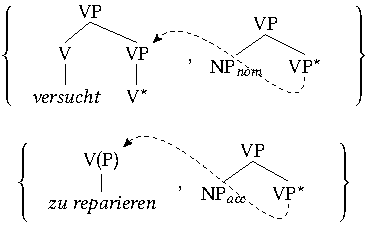
\includegraphics{graphics/abb741.pdf}
\caption{\label{fig-ttmctag-vtag-1}V-TAG-Baummenge für die Modellierung des 1.~Grenzfalls in \ref{ex-ttmctag-vtag-1} mit Scrambling im Mittelfeld}
\end{figure}

Ähnliches gilt für den zweiten Grenzfall, eine Kombination aus partieller Voranstellung\is{Voranstellung!partielle} des infiniten Verbs und der Platzierung seiner Ergänzung im Mittelfeld wie in \ref{ex-ttmctag-vtag-2}:

\ex. Zu reparieren versucht ihn Peter. \label{ex-ttmctag-vtag-2}

Auch hier reicht eine reguläre V-TAG zur Derivation aus, wie die Baummengen in Abbildung~\ref{fig-ttmctag-vtag-2} zeigen. Dabei handelt es sich bei den Elementarbäume in den Baummengen um genau jene, die bereits für TT-MCTAG mit Spine-Sharing-Lokalität vorgeschlagen wurden.
\begin{figure}[t]
\centering
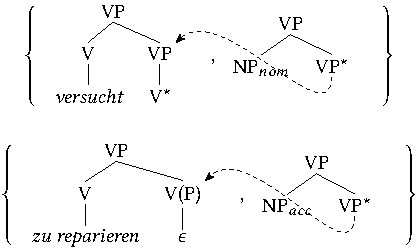
\includegraphics{graphics/abb742.pdf}
\caption{\label{fig-ttmctag-vtag-2}V-TAG-Baummenge für die Modellierung des 2.~Grenzfalls in \ref{ex-ttmctag-vtag-2} mit einfacher partieller Voranstellung}
\end{figure}
Es scheint also so zu sein, dass V-TAG unter diesen Rahmenbedingungen mindestens so ausdrucksstark ausfällt wie TT-MCTAG\is{TT-MCTAG} mit Spine-Sharing-Lokalität\is{Spine Sharing}. 

%\subsubsection*{Dritter Grenzfall}

Der dritte Grenzfall, d.\,h.\ eine mehrfach partielle Voranstellung\is{Voranstellung!partielle} wie in \ref{ex-ttmctag-vtag-3}, stellt an TT-MCTAG höhere Anforderungen als der erste und zweite Grenzfall. Eine Spine-Sharing-Loka\-li\-tät alleine reicht zur Modellierung nicht aus:

\ex. Zu reparieren versprochen hat ihm das Peter. \label{ex-ttmctag-vtag-3}

Doch auch V-TAG scheint dem dritten Grenzfall nicht ohne Weiteres gewachsen zu sein. Zwar kann eine Phrasenstruktur ohne \isi{Vorfeldbündelung} (siehe Abbildung~\ref{fig-ttmctag-grenzen-iii-4}) mit den Baummengen in Abbildung~\ref{fig-ttmctag-vtag-3}  generiert werden, aber die Modellierung der Vorfeldbündelung verlangt eine Anpassung anderer Art. 
\begin{figure}[t]
\centering
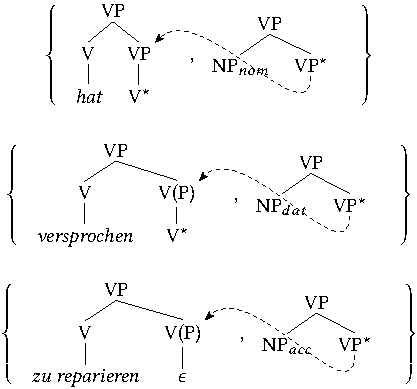
\includegraphics{graphics/abb743.pdf}
\caption{\label{fig-ttmctag-vtag-3}V-TAG-Baummenge für die Modellierung des 3.\ Grenzfalls in \ref{ex-ttmctag-vtag-3} mit mehrfach partieller Voranstellung ohne Vor"-feld"-bündelung}
\end{figure}
Ein Beispiel dafür ist in den Baummengen in Abbildung \ref{fig-ttmctag-vtag-4} zu sehen.
\begin{figure}[t]
\centering
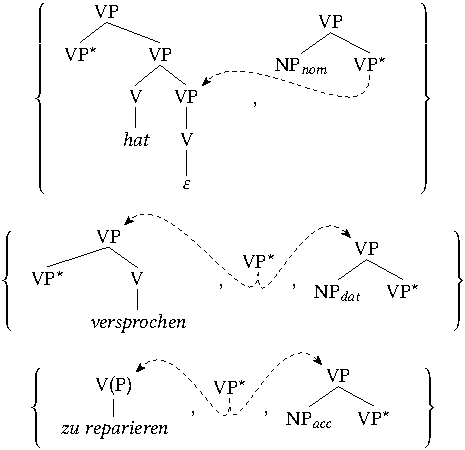
\includegraphics{graphics/abb744.pdf}
\caption{\label{fig-ttmctag-vtag-4}V-TAG-Baummenge für die Modellierung des 3.~Grenzfalls in \ref{ex-ttmctag-vtag-3} mit mehrfach partieller Voranstellung mit Vor"-feld"-bündelung}
\end{figure}
Mit ihrer Hilfe gelingt die Derivation von \ref{ex-ttmctag-vtag-3} mit Vorfeldbündelung und ohne vom Phrasenstrukturprinzip\is{Wohlgeformtheitsprinzip!Phrasenstrukturprinzip} in anderer Hinsicht abweichen zu müssen. Das Besondere an diesen Baummengen ist der zusätzliche Hilfsbaum, der nur aus einem Knoten besteht und jeweils mit Dominanzlinks auf die anderen Elementarbäume versehen ist. Sie werden am Wurzelknoten des {\it hat}-Baums adjungiert und dominieren damit sowohl das infinite Verb als auch dessen Ergänzung. Problematisch daran ist weniger die Tatsache, dass es sich um unlexikalisierte Elementarbäume handelt, als dass es einknotige Hilfsbäume sind. Eine der grundlegenden Konventionen des TAG-Formalismus besteht nämlich darin, dass an den Fu\ss knoten nicht adjungiert werden darf (siehe Abschnitt \ref{sec-ttmctag-formalismus}). Demzufolge ist es also gar nicht möglich, nacheinander zwei einknotige Hilfsbäume am Wurzelknoten des {\it hat}-Baums zu adjungieren, wie es in der Analyse von \ref{ex-ttmctag-vtag-3} nötig wäre. Ich sehe jedoch keine große Hürde darin, eine Ausnahme für solche einknotigen Hilfsbäume zu stipulieren.\footnote{Als unschön könnte man (neben der Stipulation als solcher) die Tatsache bewerten, dass dieser Ansatz zu falscher derivationeller Ambiguität führt, d.\,h.\ für ein und denselben abgeleiteten Baum\is{abgeleiteter Baum} gibt es mehrere mögliche Ableitungsbäume\is{Ableitungsbaum}.} Schwerwiegender sind da in meinen Augen die \isi{Fu\ss knoten} der Hilfsbäume mit NP-Blatt: Von ihnen geht kein \isi{Dominanzlink} aus, sie müssen also qua Valenzprinzip\is{Wohlgeformtheitsprinzip!Valenzprinzip für V-TAG} durch den Valenzrahmen des lexikalischen Ankers lizenziert sein, was hier aber nicht der Fall ist. Das Valenzprinzip müsste also ebenfalls angepasst werden, etwa indem der valenztheoretische Status eines Fu\ss knotens nicht aus der Existenz eines Dominanzlinks folgt, sondern explizit stipuliert werden muss.\footnote{Würde man stattdessen einen Dominanzlink vom Fußknoten des NP-Slots zu einer Spur des vorangestellten Kopfes annehmen, bestünde das Problem auch, nur an anderer Stelle.}

Zusammenfassend lässt sich also sagen, dass die V-TAG-Modellierung des 3.\ Grenzfalls Unzulänglichkeiten zeigt, deren Behebung grö\ss ere Eingriffe im System der Wohlgeformtheitsprinzipien erfordert. Die Annahme einer Tree"=Sharing"=Lokalität\is{Tree Sharing} bei TT-MCTAG scheint mir im Vergleich dazu das kleinere Übel zu sein.
\is{Vector-MCTAG (V-TAG)|)}


\section{Besser eine spinalisierte Variante?}\label{sec-ttmctag-spinal}\is{TT-MCTAG!spinalisierte|(}

Wir haben gesehen, dass TT-MCTAG mit Tree-Sharing-Lokalität für eine umfangreiche Modellierung kohärenter Konstruktionen eingesetzt werden kann. Selbst eine Modellierung der mehrfach partiellen Voranstellung ist möglich, ohne beim Valenzprinzip oder beim Phrasenstrukturprinzip Zugeständnisse machen zu müssen. Dies ist ein sehr erfreuliches Ergebnis und führt die TAG-Forschung endlich an das Niveau vergleichbarer HPSG-Forschung heran, die in dieser Arbeit ausgiebig zitiert wurde.

\subsection{Verbliebene Desiderata}

Doch so positiv dieses Ergebnis auch sein mag, es bleiben für mich Desiderata bestehen, die jenseits der Aspekte technischer Machbarkeit interessant werden:\footnote{Die folgenden Überlegungen wurden teilweise bereits in \cite{Lichte:10} gemacht.}
\begin{enumerate}\label{enum-ttmctag-spinal}
  \item Im Zusammenhang mit der Anpassung der \isi{Phrasenstruktur} in Abschnitt \ref{sec-ttmctag-grenzen-anpassung} habe ich bemerkt, dass sich aus den Grundprinzipien der TT"=MCTAG"=Modellierung keine Entscheidung zwischen links- und rechtsverzweigendem Mittelfeld herbeiführen lässt. Diese Strukturalternativen scheinen prinzipiell gleichwertig. Wie ich daraufhin schloss, zeigt deren Gleichwertigkeit, dass hier eine Struktureigenschaft variiert, die nicht benötigt wird, und die im Sinne des Ockhamschen Rasiermessers entfernt werden sollte: Lässt sich irgendwie eine grö\ss ere Verbindlichkeit der \isi{Phrasenstruktur} herstellen?
  \item Die TT-MCTAG-Modellierung soll prinzipiell ohne leere Elemente\is{leere Kategorie} auskommen, benötigt diese aber bisweilen aus  technischen Gründen in der rechten Satzklammer: Lassen sich diese leeren Elemente irgendwie vermeiden?
  \item Das topologische Felderschema\is{topologische Felder} und andere Linearisierungsgesetzmä\ss igkeiten werden mittels spezieller Linearisierungsmerkmale wie {\sc vf} implementiert, deren Verhalten bei Adjunktionen und {\sc top}"={\sc bottom}"=Unifikationen richtig antizipiert werden muss:  Gibt es einen intuitiveren Weg der Implementierung von Linearisierungsgesetzmä\ss igkeiten\is{Linearisierung}?
  \item Für unterschiedliche syntaktische Stellungen werden häufig unterschiedliche Baumtupel stipuliert: Wie lässt sich der Zusammenhang zwischen solchen Baumtupeln darstellen oder eine gemeinsame Repräsentation solcher Baumtupel finden? 
\end{enumerate} 

Zunächst soll die Überlegung angestellt werden, wie die abgeleitete Struktur ohne verzweigendes Mittelfeld und ohne leeres Element aussehen könnte, die durch eine noch zu bestimmende TT-MCTAG-Variante generiert werden soll. Dafür konzentriere ich mich auf die mehrfach partielle Voranstellung\is{Voranstellung!partielle}, die sich in den vorangegangenen Abschnitten als besondere Herausforderung für den TT-MCTAG-Ansatz erwiesen hat. Statt der Phrasenstruktur in Abbildung~\ref{fig-ttmctag-grenzen-iii} nehme ich die Phrasenstruktur\is{Phrasenstruktur!flache} in Abbildung~\ref{fig-ttmctag-spinal-1} an. 
\begin{figure}[t]
\centering
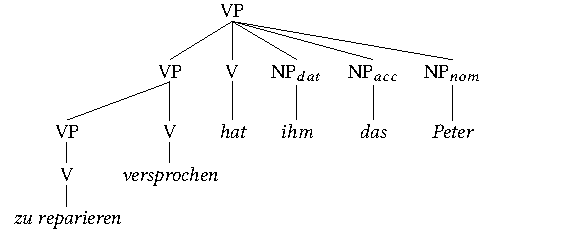
\includegraphics{graphics/abb745.pdf}
\caption{\label{fig-ttmctag-spinal-1}Flacher abgeleiteter Baum für eine mehrfach partielle Voran"-stellung}
\end{figure}
Sie behält die \isi{Vorfeldbündelung} bei, enthält aber nur einen VP-Knoten, der alle Vorfeld- und Mittelfeldknoten aus Abbildung \ref{fig-ttmctag-grenzen-iii} vereinigt. Dadurch erhalten wir einen flachen, nicht-binären Baum ohne mehrstufige VP-Projektion über dem Mittelfeld. Auf die Repräsentation der leeren rechten \isi{Satzklammer} wird verzichtet.     

Wie sich flache Phrasenstrukturen\is{Phrasenstruktur!flache} dieser Art erzeugen lassen, wurde bereits für GPSG\is{Generalized Phrase Structure Grammar (GPSG)} \citep{Uszkoreit:86,Uszkoreit:87} und HPSG\is{Head-driven Phrase Structure Grammar (HPSG)} \citep{Pollard:96} beschrieben.\footnote{In diesen Ansätzen ist allerdings die Anzahl der benötigten Regeln sehr gro\ss, unter Umständen sogar unendlich, da auch Angaben\is{Angabe} integriert werden müssen \citep[Abschnitt~2.2.1]{Mueller:04}.} Eine reguläre TT-MCTAG (oder LTAG) scheint mir dazu jedoch nicht in der Lage zu sein, ohne das Valenzprinzip in der jetzigen Form au\ss er Kraft zu setzen. Dafür fehlt hier schlicht die durch die \isi{Adjunktion} hervorgerufene Rekurrenz aus Wurzel- und Fu\ss knoten, d.\,h.\ die eben zusammengefasste mehrgliedrige VP-Projektion aus Vor- und Mittelfeldknoten. Es stellt sich also die Frage, welche Verknüpfungsoperation Strukturen wie in Abbildung~\ref{fig-ttmctag-spinal-1} erzeugen kann und zugleich eine valenztheoretisch befriedigende Analyse im Rahmen von TT-MCTAG zulässt.

\subsection{Spinal-TT-MCTAG und Fusion} 

Die Antwort, die ich hier darauf geben möchte, erschlie\ss t sich bei einem Blick auf die Ableitung (oder Elementarbaum-Partition) in Abbildung~\ref{fig-ttmctag-spinal-3}.\footnote{Dies stellt natürlich nicht die einzig mögliche Ableitung dar. Ein alternatives System basierend auf \isi{Sister Adjunction} wird in \cite{Lichte:10} diskutiert.} 
\begin{figure}[t]
\centering
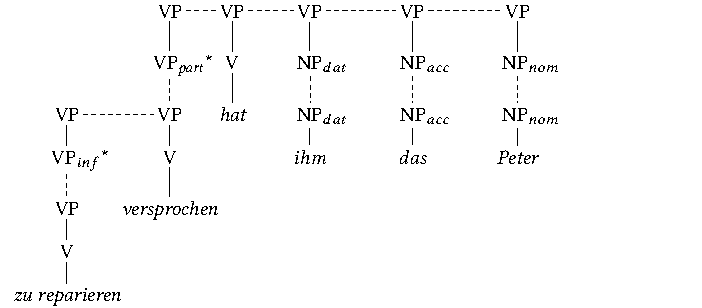
\includegraphics{graphics/abb746.pdf}
\caption{\label{fig-ttmctag-spinal-3}Eine Elementarbaum-Partition der flachen Phrasenstruktur in Abbildung~\ref{fig-ttmctag-spinal-1}}
\end{figure}
Auf Grundlage der hier verwendeten Elementarbäume lassen sich die Tupel in Abbildung~\ref{fig-ttmctag-spinal-3} erstellen.  
\begin{figure}[t]
\centering
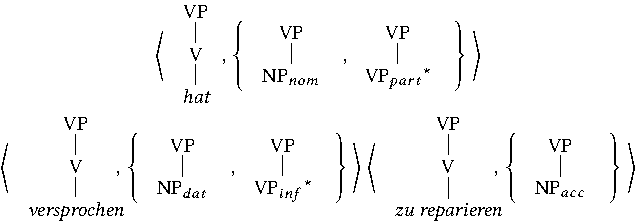
\includegraphics{graphics/abb747.pdf}
\caption{\label{fig-ttmctag-spinal-4}Baumtupel für die Elementarbaum-Partition in Abbildung~\ref{fig-ttmctag-spinal-1}}
\end{figure}
Zunächst fällt auf, dass die Elementarbäume allesamt unär sind, was in Anlehnung an \cite{Shen:06} und \cite{Shen:etal:08} Spinalisierung genannt wird.\footnote{Die Terminologie ist leider unglücklich gewählt, da man als \isi{Spine} auch den Pfad vom Fu\ss knoten zum Wurzelknoten bezeichnet, so etwa in \cite{Schabes:Waters:95}.} Die Spinalisierung der Elementarbäume ist ein charakteristisches (jedoch nicht zwingend notwendiges) Merkmal dieser TT-MCTAG-Variante, weshalb ich im Folgenden auch von \textsc{Spinal-TT-MCTAG} sprechen werde. Die waagrechten gestrichelten Linien stehen für eine neuartige Verknüpfungsoperation, die ich \textsc{Fusion}\is{Fusion} nennen möchte: Wenn zwei Knoten $v_i,v_j$ aus den Bäumen $\gamma_i,\gamma_j$ fusioniert werden, dann werden sie im resultierenden Baum $\gamma'$ durch einen Knoten $v'$ ersetzt, für den gilt, dass (i) alle direkt dominierenden Knoten von $v_i, v_j$ nun $v'$ direkt dominieren und (ii) die durch $v_i,v_j$ dominierten Teilbäume unmittelbar adjazent sind und $v'$ ausschlie\ss lich diese Teilbäume dominiert.   
Eine formale Definition befindet sich weiter unten in diesem Abschnitt. Drei Einschränkungen für den Gebrauch der \isi{Fusion} kommen noch hinzu: (i) die Knotenlabels der fusionierten Knoten müssen identisch sein; (ii) mindestens einer der fusionierten Knoten muss ein Wurzelknoten sein, um die Baumförmigkeit der abgeleiteten Struktur zu erhalten; (iii) es können nur \isi{Innenknoten} fusioniert werden.\footnote{Die Fusion kann als eingeschränkte Form der \isi{Baumunifikation} verstanden werden, die bei TUG verwendet wird \citep{Popowich:89,Gerdes:04}. Siehe dazu auch Abschnitt~\ref{sec-stug-intro}.} 

Neben der \isi{Fusion} stehen weiterhin Substitution und Adjunktion zur Verfügung, die für die Ersetzung nicht-terminaler Blätter benötigt werden und sich nur in der Rolle der Lokälitätsbestimmung im Rahmen der Sharing-Lokalität unterscheiden: Die \isi{Substitution} definiert Lokalitätsinseln, während die \isi{Adjunktion} die Lokalitätsdomäne per Sharing erweitert. Da mit der \isi{Fusion} eine Verknüpfungsoperation für Angaben/Modifizierer\is{Angabe} schon zur Verfügung steht, kann die Adjunktion so eingeschränkt werden, dass Hilfsbäume nur am Wurzelknoten des Zielbaums adjungieren dürfen. Dies hat durchaus erfreuliche Folgen für den Ableitungsbaum, wie wir gleich sehen werden. Blicken wir aber zunächst mit diesem Wissen auf die Tupel der experimentellen Spinal-TT-MCTAG in Abbildung \ref{fig-ttmctag-spinal-4}. 
Im Unterschied zu TT-MCTAG zeigen die Fu\ss knoten der Hilfsbäume in der Argumentbaummenge Ergänzungen\is{Ergänzung} des lexikalen Kopfes an. Das bedeutet, dass nicht nur diejenigen Argumentslots, die sich wie Inseln\is{Bewegungsinsel} verhalten und als \isi{Substitutionsknoten} angedeutet sind, in der Argumenbaummenge erscheinen,  sondern auch jene verbalen Ergänzungen, mit denen der valenztragende Kopf kohärent konstruiert. Da mehr als eine Ergänzung als Fu\ss knoten angedeutet sein kann, erlaubt es Spinal-TT-MCTAG im Unterschied zu TT-MCTAG, mehr als eine disjunkte Ergänzung abzuleiten.  

Entsprechend der Tupel-Idee, müssen die Argumentbäume\is{Argumentbaum} mit dem \isi{Kopfbaum} im Laufe der Ableitung verknüpft werden -- direkt oder indirekt über Node"=Sharing\is{Node Sharing}. Als direkte Verknüpfung zählt bei Spinal-TT-MCTAG die \isi{Fusion} von Kopfbaum und Argumentbaum. In Abbildung~\ref{fig-ttmctag-spinal-3} trifft das beispielsweise auf den {\it versprochen}-Baum und den VP$_{\mathit{inf}}$-Hilfsbaum zu. Die Verknüpfung des {\it versprochen}"=Baums mit dem NP$_{\mathit{dat}}$-Baum erfolgt dagegen indirekt, indem der NP$_{\mathit{dat}}$-Baum mit einem Hilfsbaum fusioniert, der am Wurzelknoten des {\it versprochen}-Baums adjungiert. Dies entspricht der TT-MCTAG-Intuition des Node Sharings\is{Node Sharing}: Der Wurzelknoten eines Hilfsbaums $\gamma_1$, der an einem Elementarbaum $\gamma_2$ adjungiert, wird also von $\gamma_1$ und $\gamma_2$ geshared.

\subsection{Ableitungsbäume}

Auch bei Spinal-TT-MCTAG kann die Festlegung der Node-Sharing-Loka\-li\-tät\is{Node Sharing} anhand des Ableitungsbaums\is{Ableitungsbaum} erfolgen. Dieser weicht jedoch von den Ableitungsbäumen einer TT-MC\-TAG wesentlich ab. Ursache dafür ist die \isi{Fusion}, die im Unterschied zu Adjunktion und Substitution als symmetrische Verknüpfung verstanden werden muss, d.\,h.\ als eine Verknüpfung derivationell gleichwertiger Bäume. Man kann hier nicht davon sprechen, dass einer der Bäume die Verknüpfung irgendwie hervorruft oder einen Knoten des anderen Baumes ersetzt.\footnote{Vgl.\ auch die Bemerkung von \citet[21]{Gerdes:04} zu Ableitungsbäumen in TUG\is{Tree Unification Grammar (TUG)}, wo ja ebenfalls Knoten unifiziert werden: "`In  standard TAG, the derivation tree just records which node was substituted or adjoined into which other node. The case for TUG is less simple, as the atom unification is not directional, not unique, and non-local in the sense that an elementary tree can unify with branches `belonging' to different elementary trees."' } Allein die lineare Abfolge der beteiligten Bäume stellt so etwas wie Asymmetrie her. Ich schlage deshalb vor, im \isi{Ableitungsbaum} die \isi{Fusion} als Kette (d.\,h.\ als spinalisierten Teilableitungsbaum) darzustellen, und diese Ketten als Knoten des Ableitungsbaums zu betrachten. Die Ableitung in Abbildung~\ref{fig-ttmctag-spinal-3} soll also durch den Ableitungsbaum in Abbildung~\ref{fig-ttmctag-spinal-5} repräsentiert werden. Man beachte, dass die Fusionsketten dann einelementig sind, wenn keine Fusion stattfindet.\footnote{Eine interessante Beobachtung lässt sich hier machen: Der abgeleitete Baum\is{abgeleiteter Baum} und der \isi{Ableitungsbaum} gleichen sich einander an, auch wenn natürlich nach wie vor Unterschiede bestehen. Möglicherweise ist der Idealfall einer, in dem der abgeleitete Baum und der Ableitungsbaum übereinstimmen, der Ableitungsbaum also direkt generiert wird.} 
\begin{figure}[t]
\centering
\includegraphics{graphics/abb748.pdf}
\caption{\label{fig-ttmctag-spinal-5}Ableitungsbaum mit Fusionsketten für die Ableitung in Abbildung~\ref{fig-ttmctag-spinal-4}}
\end{figure}

Eine andere wesentliche Veränderung am \isi{Ableitungsbaum} sehen wir in den Kantenlabels: Statt Gorn-Adressen\is{Gorn-Adresse} werden zur Identifizierung des Zielbaums\is{Zielbaum} die Elemente der Ketten verwendet. Das Kantenlabel \textsc{s.np$_{\mathit{dat}}$} bedeutet beispielsweise, dass eine Substitution am Elementarbaum {\tt NP$_{\mathit{dat}}$} stattfindet, einem Element der Fusionskette, von dem die Kante ausgeht. Gorn-Adressen sind bei der Repräsentation der Substitution und Wurzeladjunktion irrelevant, da ein Elementarbaum in der spinalisierten Form maximal ein nicht-terminales Blatt enthält. Bei der Repräsentation der \isi{Fusion} kann dagegen die Angabe der \isi{Gorn-Adresse} notwendig sein, falls die Fusion echt-dominierte Innenknoten betrifft. Ich klammere diesen Fall hier aus, um die Darstellung nicht unnötig komplizierter zu machen.

Schlie\ss lich besteht eine wesentliche Neuerung hinsichtlich der Form des Ableitungsbaums\is{Ableitungsbaum} darin, dass Hilfsbäume\is{Hilfsbaum} (bzw.\ die Ketten, die sie enthalten) ihre Zielbäume\is{Zielbaum} dominieren. Da nur Wurzeladjunktionen möglich sind, kommen dadurch keine mehrwurzligen Ableitungsbäume zustande und man vermeidet sie sogar in Situationen, wo eine Fusionskette mehrere Hilfsbäume enthält. Ein willkommener Nebeneffekt dieser Repräsentation besteht au\ss erdem darin, dass sich Spinal-TT-MCTAG-Ableitungsbäume und die entsprechenden Dependenzgraphen\is{Dependenzgraph} strukturell etwas annähern.\footnote{Trotz der Beschränkung auf Wurzeladjunktion können weite Abhängigkeiten (z.\,B.\ Brückenkonstruktionen\is{Brückenkonstruktion}) erfasst werden. Die Platzierung der Brückenverben zwischen Filler und Gap ermöglicht die Fusionsoperation.}

Diese Umkehrung der Adjunktionskanten erinnert an das Vorgehen bei der "`flexible composition"'\is{Flexible Composition} bzw.\ "`reversed adjunction"' (\citealt{Joshi:etal:03, Kallmeyer:Joshi:03, Chiang:Scheffler:08}): Der Hilfsbaum kann dort optional als Zielbaum der Adjunktionsoperation fungieren, dessen Fu\ss knoten dann ähnlich wie ein Substitutionsknoten behandelt wird. Da die klassische Adjunktionsvariante weiterhin zur Verfügung steht, sind die Umkehrungen der Adjunktionskanten nicht trivial, d.\,h.\ es können Kanten nicht nur umgekehrt, sondern auch umgesetzt werden. Genau das ist auch erwünscht, um bestimmte Phänomene mit einer baumlokalen MCTAG\is{Multi-Component TAG (MCTAG)!baumlokale (TL-MCTAG)} behandeln zu können (siehe \cite{Chiang:Scheffler:08} für eine Übersicht).\footnote{Eine alternative Sichtweise auf die "`flexible composition"'\is{Flexible Composition} ohne Kantenumkehrung im Ableitungsbaum schlagen \cite{Chiang:Scheffler:08} mit der "`delayed tree-locality"' vor. Die Elementarbäume einer Baummenge müssen dort nicht unmittelbar mit demselben Elementarbaum verknüpft werden, sondern können dies mit einer bestimmten Verzögerung.} Im Unterschied dazu ist die hier vorgeschlagene Umkehrung der Adjunktionskanten rein notationeller Art, denn (i) die \isi{Adjunktion} kann ausschlie\ss lich am \isi{Wurzelknoten} vollzogen werden und (ii) die Umkehrung der Adjunktionskanten im Ableitungsbaum ist obligatorisch, nicht optional.

\subsection{Node-Sharing-Lokalität}

Diese auf das wesentliche beschränkte Darstellung der zentralen Eigenschaften von Spinal-TT-MCTAG-Ableitungsbäumen genügt, um eine Anpassung der Node-Sharing-Lokalität\is{Node Sharing} vorzunehmen: Ein Argumentbaum $\beta$ fusioniert mit seinem Kopfbaum $\gamma$ Node-Sharing-lokal, falls im Spinal-TT-MCTAG-Ablei\-tungs\-baum $\beta$ entweder einer Fusionskette angehört, deren Mitglied auch $\gamma$ ist, oder falls $\beta$ einer Fusionskette angehört, die die Fusionskette mit $\gamma$ entlang eines Kantenpfads dominiert, der ausschlie\ss lich aus Wurzeladjunktionen besteht.\footnote{Könnten die Argumentbäume auch mit echt-dominierten Innenknoten der Hilfsbäume fusionieren? Nein, denn eine solche \isi{Fusion} wird im Ableitungsbaum wie eine Substitution repräsentiert. Auf diese Form der Fusion möchte ich hier, wie bereits angekündigt, nicht genauer eingehen.} Im Ableitungsbaum in Abbildung~\ref{fig-ttmctag-spinal-5} besteht beispielsweise der Pfad zwischen dem Argumentbaum {\tt NP$_{\mathit{acc}}$} und seinem Kopfbaum {\tt zu\_reparieren} aus Kanten mit den Labeln {\tt A.VP$_{\mathit{part}}$} und {\tt A.VP$_{\mathit{inf}}$} und erfüllt damit die Kriterien der Node"=Sharing"=Lokalität. 

Dass eine solche Node-Sharing-Lokalität\is{Node Sharing} auch für den Argumentbaum {\tt NP$_{\mathit{dat}}$} und den Kopfbaum {\tt versprochen} besteht, beweist die Modellierbarkeit der mehrfach partiellen Voranstellung\is{Voranstellung!partielle} durch eine Spinal-TT-MCTAG -- und das im Geltungsbereich eines Valenzprinzips, das das ursprüngliche Valenzprinzip für TT-MCTAG (vgl.\ \ref{ex-valenzprinzip-mctag}) nur unwesentlich abwandelt:\is{Wohlgeformtheitsprinzip!Valenzprinzip für Spinal-TT-MCTAG}

\ex. \label{ex-valenzprinzip-spinal-tt-mctag}{\bf Valenzprinzip (für Spinal-TT-MCTAG)} \\ 
Baumtupel entsprechen genau einem Valenzrahmen, wobei gilt:
\a. Der lexikalische Anker im Kopfbaum ist der Valenzträger.
\b. Es besteht ein bijektives Abbildungsverhältnis zwischen Valenzrollen einerseits und Substitutions- und Fu\ss knoten in der Elementarbaummenge andererseits.

Die Rolle des Kopfbaums und der nicht-terminalen Blätter kann im Valenzprinzip für Spinal-TT-MCTAG klarer charakterisiert werden.

Mit der hier skizzierten Spinalisierung von TT-MCTAG und der Einführung der Fusion als einer symmetrischen Verknüpfunsoperation scheint es also möglich, flache Phrasenstrukturen\is{Phrasenstruktur!flache} ohne leere Elemente\is{leere Kategorie} wie in Abbildung~\ref{fig-ttmctag-spinal-1} zu erzeugen und dabei die Modellierung von Lokalitätsdomänen per Node Sharing \is{Node Sharing} beizubehalten, die oben für TT-MCTAG ausgearbeitet worden ist. Das erste und zweite Desideratum auf Seite \pageref{enum-ttmctag-spinal} ist damit ansatzweise berücksichtigt. Wie steht es aber um das dritte und vierte Desideratum? Dazu kommen wir jetzt, wenn wir uns die Fusion und eine mögliche Methode ihrer Regulierung genauer anschauen.   
 

\subsection{Regulierung der Fusion}

Substitution und Adjunktion werden üblicherweise durch die Unifikation von Merkmalsstrukturen\is{Merkmalsstruktur} reguliert, wie oben bei der TT-MCTAG-Modellierung in einiger Ausführlichkeit zu sehen war. Möglicherweise lässt sich diese Form der Regulierung mehr oder weniger direkt auf die \isi{Fusion} übertragen. Die Fusion ermöglicht jedoch auch eine ganz andere Form der Regulierung, nämlich \textsc{endliche Automaten}\is{endlicher Automat}. Endliche Automaten zeichnen sich durch zwei Eigenschaften aus:

\begin{enumerate}
  \item Endliche Automaten können Abfolgen kompakt und überschaubar darstellen. Dagegen führt die Regulierung qua Merkmalstrukturen eine dezentrale Darstellung mit sich, indem Abfolgeaspekte unterschiedlichen Merkmalen zugeordnet sind, deren Wikungsweise sich erst im Zusammenspiel unterschiedlicher Elementarbäume erschlie\ss t.
\item Endliche Automaten können Abfolgealternativen zusammenfassen. Damit fällt die Stipulierung unterschiedlicher Elementarbäume für unterschiedliche Abfolgetypen weg. 
\end{enumerate}

Diese Eigenschaften lassen vermuten, dass sich die Grammatik wesentlich kompakter und gleichzeitig transparanter darstellen lässt, wodurch auch die Grammatikentwicklung und -implementierung wesentlich leichter fallen sollte.\footnote{Vgl.\ auch die Darstellung der Vorteile von Augmented Transition Networks (ATNs)\is{Augmented Transition Network (ATN)} in \citet[599ff]{Woods:70}. ATNs basieren auf dem Konzept endlicher Automaten, besitzen aber die Ausdrucksstärke von Turingmaschinen.} 
Aus meiner Sicht macht das den architektonischen Nachteil mehr als wett, nämlich dass zu den Merkmalsstrukturen, die weiterhin zur Verfügung stehen sollen, eine weitere Modellierungsstruktur hinzukommt. 

Die Verbindung zwischen dem Knoten eines Elementarbaums und einem endlichen Automaten\is{endlicher Automat} wird durch das Knotenlabel und der Funktion $\mathit{fsa}$ hergestellt, indem $\mathit{fsa}$ etwa das Knotenlabel VP auf den endlichen Automaten in Abbildung~\ref{fig-fsa} abbildet.
\begin{figure}[t]
\centering
\begin{tikzpicture}[->,>=stealth',shorten >=1pt,auto,node distance=2.8cm,
                    semithick]
  \tikzstyle{every state}=[draw=black,text=black]

  \node[initial,initial text={},state] (A) {$z_0$};
  \node[state]         (B) [right of=A]   {$z_1$};
  \node[state,accepting]         (C) [right of=B]    {$z_2$};

  \path (A) edge node {\textsc{ap|np|vp}} (B)
        (B) edge node {\textsc{v}$_{\text{fin}}$} (C)
        (C) edge [loop above] node {\textsc{ap|np|vp}} (B);
\end{tikzpicture}
\caption{\label{fig-fsa}Skizze eines endlichen Automaten für das Knotenlabel VP}
\end{figure} 
Dieser ist mit seinen drei Zuständen natürlich grob vereinfacht und erfasst gerade mal V2-Sätze\is{Satz!V2-}. Man sieht aber sehr deutlich, wie die Besetzung des Vorfelds\is{Vorfeld} mit genau einem Satzglied erzwungen werden kann: Vom Startzustand $z_0$ ausgehend muss in der Eingabe zunächst etwas von der Kategorie AP, NP oder VP stehen, um in den nächsten Zustand $z_1$ zu gelangen. Hier wird nur genau ein V$_{\mathit{fin}}$ akzeptiert, die Kategorie eines finiten Verbs. Im Endzustand $z_2$ wird schlie\ss lich eine beliebige Anzahl von  APs, NPs oder VPs akzeptiert.   

AP, NP, VP und V$_{\mathit{fin}}$ habe ich gerade als Kategoriebezeichnungen geführt. Es sind aber tatsächlich Knotenlabel. Die Eingabe für den endlichen Automaten\is{endlicher Automat}, der per Knotenlabel an den Knoten $v$ eines abgeleiteten Baums geknüpft ist, bildet die Konkatenation derjenigen Knotenlabel, die unmittelbar von $v$ dominiert werden. Wir definieren dafür die Funktion $\mathit{idom}$, die einen Knoten auf eine Knotenlabelkonkatenation abbildet. Für jeden Knoten $v$ eines wohlgeformten abgeleiteten Baums soll dann gelten: $\mathit{idom}(v) \in L(\mathit{fsa}(l_V(v)))$, wobei $l_V$ die Labelfunktion über Knoten ist, d.\,h.\ $l_V (v)$ ist das Label von $v$.   
 
Die Verwendung endlicher Automaten\is{endlicher Automat} bei der Modellierung der Syntax natürlicher Sprache ist unüblich.\footnote{Gemeint ist hier nicht der Parser für solche Syntaxmodelle. Manche TAG-Parser\is{Parsing} verwenden sehr wohl endliche Automaten\is{endlicher Automat} für bestimmte Teilaspekte, z.\,B.\ zur internen Repräsentation von Baumschablonen und Elementarbäumen \citep{Nasr:Rambow:04} oder zur lexikalischen Disambiguierung vor dem eigentlichen Parsen \citep{Gardent:etal:14}. Dank an Owen Rambow für den Hinweis!} Ein Grund dafür liegt sicherlich in deren unzulänglicher Ausdrucksstärke, die nur die Generierung von regulären Sprachen zulässt. Doch auch die in \cite{Woods:70} vorgeschlagenen Varianten, die Recursive Transition Networks\is{Recursive Transition Network (RTN)} für die Generierung kontextfreier Sprachen und die Augmented Transition Networks\is{Augmented Transition Network (ATN)} mit einer der \isi{Transformationsgrammatik} entsprechenden Ausdrucksstärke, genie\ss en heutzutage bestenfalls den Status historischer Fu\ss noten. In der vorliegenden Arbeit dienen endliche Automaten\is{endlicher Automat} zur Modellierung eines bestimmten Teilbereichs der Syntax, nämlich der \isi{Linearisierung} von nicht-terminalen Schwesterknoten. Erstaunlicherweise trifft man selbst auf solche im syntaktischen Modell eingebettete endliche Automaten nur überaus selten.\footnote{Eine Arbeit dieser Art ist z.\,B.\ \cite{Maxwell:Manning:96}, wo im Rahmen einer LFG\is{Lexical-Functional Grammar (LFG)} endliche Automaten für die Repräsentation der rechten Seite einer c-Struktur-Regel genutzt werden, um bei der Modellierung der Konstituentenkoordination von der konkreten morphosyntaktischen Form der Konjunkte abstrahieren zu können.} Angesichts der oben erwähnten Vorteile, nämlich Kompaktheit und Transparenz, erscheint mir diese Ignoranz als ungerechtfertigt.

Zum Schluss möchte ich noch auf einen anderen, sehr interessanten Aspekt von Spinal-TT-MCTAG hinweisen: Es scheint mir hier ein inkrementeller Grammatikformalismus\is{Inkrementalität} vorzuliegen, dessen Derivationen der "`full connectivity"' \citep{Sturt:Lombardo:05} bzw.\ "`strong connectivity"' \citep{Stabler:94} genügen. Das bedeutet, dass für jedes Präfix einer Eingabe eine (unfertige) zusammenhängende syntaktische Repräsentation generiert werden kann. Damit würde Spinal-TT-MCTAG zu den inkrementellen TAG-Versionen wie DVTAG \citep{Mazzei:etal:07} und PLTAG \citep{Demberg:Keller:08, Demberg:10} zählen. 


\subsection{Definitionen}

Die vorangegangenen informellen Erläuterungen des Spinal"=TT"=MCTAG"=Formalismus sollen nun formal expliziter gemacht werden. Zunächst kann eine spinalisierte TT-MCTAG als TT-MCTAG mit einer Funktion $\mathit{fsa}$ definiert werden: 
\begin{definition}[Spinal-TT-MCTAG]
Sei $G = \langle N,T,S,I,A,\mathcal{A},h\rangle$ eine TT"=MCTAG. $G' = \langle N,T,S,I,A,\mathcal{A},h,\mathit{fsa}\rangle$ ist eine spinalisierte TT"=MCTAG (Spinal"=TT"=MCTAG) mit $\mathit{fsa} = N \to M$, wobei $M$ die Menge der endlichen Automaten ist.
\end{definition}
Die Bedeutung der endlichen Automaten\is{endlicher Automat} für die Zulässigkeit eines abgeleiteten Baums bestimmt die folgende Definition:
\begin{definition}[Abgeleiteter Baum einer Spinal-TT-MCTAG]
Sei $D = \langle V,E\rangle$ ein abgeleiteter Baum einer Spinal-TT-MCTAG $G = \langle N,T,S,I,A,\mathcal{A},h,\mathit{fsa}\rangle$ mit einer partiellen Präzedensrelation $\prec$ über $V$ und einer Beschriftungsfunktion $l_V = V \times N \cup T$. Sei ferner $\mathit{dtrs}$ eine Abbildung von Knoten auf die Konkatenation der Label der unmittelbar dominierten Knoten, also: \\[-1ex]

\noindent$\mathit{dtrs} = \{ (v, l_V(v_1)\ldots l_V(v_n)) |$ \\[-4ex]
\begin{itemize}
  \item[] $v, v_1, \ldots, v_n \in V$, \\
  $(v,v_i) \in E$ für $1 \leq i \leq n$, \\
  $\forall v'$ mit $(v,v') \in E$, $v' \in \{v_1, \ldots, v_n\}$, \\ 
  $(v_{i-1}, v_i) \in \ \prec$ für $1 < i \leq n$ \\[1.5ex] 
  $\}$	
\end{itemize}
Dann gilt: $\forall v \in V [ \mathit{dtrs}(v) \in L( \mathit{fsa}(l_V(v))) ]$.
\end{definition}
Die Konkatenation der Label der unmittelbar dominierten Knoten eines Knotens $v$, d.\,h.\ der Tochterlabelstring $\mathit{dtrs}(v)$, soll also in der Sprache desjenigen endlichen Automaten sein, der mit dem Label von $v$ qua $\mathit{fsa}$ zusammenhängt. Ein kurzes Beispiel: Der Wurzelknoten mit VP-Label in Abbildung~\ref{fig-ttmctag-spinal-1} dominiert den Tochterlabelstring VP V NP NP NP (modulo Subskripte), und dieser ist in der Sprache des zum VP-Label zugehörigen endlichen Automaten in Abbildung~\ref{fig-fsa}.

Die Fusionsoperation\is{Fusion} kann ohne Bezug auf Spinal-TT-MCTAG und endliche Automaten folgenderma\ss en definiert werden: 
\begin{definition}[Fusion] \label{def-fusion} Seien $\gamma_i = \langle V_i,E_i \rangle$ mit der Präzedensrelation $\prec_i$ und $\gamma_j = \langle V_j,E_j \rangle$ mit der Präzedensrelation $\prec_j$ geordnete Bäume. $\gamma_i$ und $\gamma_j$ {\bf fusionieren} zu $\gamma_{ij} = \langle V_{ij}, E_{ij} \rangle$ mit $\prec_{ij}$ an den Knoten $v_i \in V_i$, $v_j \in V_j$, so dass gilt:
\begin{itemize}
  \item $\gamma_{ij}$ ist ein Baum,
  \item $V_{ij} = V_i \cup V_j \backslash v_i$,
  \item $E_{ij} = \{(v_1,v_2) \in E_i| v_1 \neq v_i \wedge v_2 \neq v_i \}$ \\
                 $~~~~~ \cup \ \{ (v_1, v_j) | (v_1,v_i) \in E_i \}$ \\
                 $~~~~~ \cup \ \{ (v_j, v_2) | (v_i,v_2) \in E_i \}$ \\
                 $~~~~~ \cup \ E_j$, 
  \item $\prec_{ij} = \{ (v_1,v_2) \in \ \prec_i| v_1 \neq v_i \wedge v_2 \neq v_i \}$ \\
                 $~~~~~ \cup \ \{ (v_1, v_j) | (v_1,v_i) \in \ \prec_i \}$ \\
                 $~~~~~ \cup \ \{ (v_j, v_2) | (v_i,v_2) \in \ \prec_i \}$ \\
                 $~~~~~ \cup \ \prec_j$ \\
                 $~~~~~ \cup \ \{ (v_i',v_j') | (v_i,v_i') \in E_i \wedge (v_j,v_j') \in E_j \ \wedge $ \\ 
                 $~~~~~~~~~~~~~~~~~~~$      es gibt kein $ (v_i',v_n) \in \ \prec_i$ \\
                 $~~~~~~~~~~~~~~~~~~~$      und kein $(v_m,v_j') \in \ \prec_j$ für beliebige $v_n, v_m \}$
\end{itemize}
\end{definition}
Zwei Bäume fusionieren\is{Fusion} an je einem ihrer Knoten, wobei der resultierende Graph wiederum baumförmig ist. Dadurch muss einer der fusionierenden Knoten ein \isi{Wurzelknoten} sein. Man beachte, dass in dieser Definition die beteiligten Bäume zunächst einmal derivationell ungleichwertig sind: Ein Knoten aus $\gamma_i$ wird durch einen Knoten aus $\gamma_j$ ersetzt, wobei durch die Bestimmung von $\prec_{ij}$ eine lineare Ordnung bezüglich den entsprechenden Teilbäumen von $\gamma_i$ und $\gamma_j$ vorgegeben ist. Diese Festlegung ist für die folgende Definition des Ableitungsbaums wesentlich. Die derivationelle Ungleichwertigkeit im Zuge der Fusion ist aber schwächer ausgeprägt als bei der Substitution oder Adjunktion, denn sie hängt nur von Aspekten der linearen Ordnung ab und ist deshalb prinzipiell umkehrbar. 

% \begin{definition}[Baum mit Ketten]
% Ein Baum mit Ketten ist ein Tupel $D = \langle V,C,E\rangle$ mit den Labelfunktionen $l_E = E \to L_E$ und $l_V = V \to L_V$, wobei $V$ die Menge der Knoten, $C$ die Menge der Ketten mit $C = V \times 2^{V \times V}$ und $E$ die Menge der Kanten mit $E = C \times C$ ist. $E$ ist ein Baum über $C$.
% \end{definition}


In der Definition eines Spinal-TT-MCTAG-Ableitungsbaums\is{Ableitungsbaum} nutze ich der Lesbarkeit wegen die folgenden Schreibweisen: $\vec{\Gamma}$ ist eine Kette von Elementarbäumen und $\vec{\Gamma}.p$ das $p$te Element von $\vec{\Gamma}$. \#$_b(\vec{\Gamma})$ ist die Anzahl der nicht-terminalen Blätter in $\vec{\Gamma}$. Desweiteren sollen die Einschränkung gelten, dass sowohl \isi{Adjunktion} als auch \isi{Fusion} nur über \isi{Wurzelknoten} operieren kann.

\begin{definition}[Spinal-TT-MCTAG-Ableitungsbaum] \label{def-spinal-ablbaum}
Sei $G = \langle N,T,S,I,A,\mathcal{A},$""$h,\mathit{fsa}\rangle$ eine Spinal-TT-MCTAG und $D = \langle  V,E \rangle $ ein Ableitungsgraph. Sei ferner $\Gamma_G$ eine Menge von Elementarbauminstanzen aus G und $V \subseteq \Gamma_G \times 2^{\Gamma_G \times \Gamma_G}$ eine Menge von Ketten über $\Gamma_G$:
\begin{itemize}
  \item $D$ ist ein Baum.
  \item Für jede Kante $\langle v_i, v_j, p \rangle \in E$ gilt: $v_i.p$ hat ein nicht-terminales Blatt. 
  \item Für jeden Knoten $v$ gilt: $|\{ \langle v, v', p \rangle \in E | v'$ und $p$ sind beliebig$ \}| = $\#$_b(v)$.
  \item Für jedes $\gamma \in \Gamma_G$ gibt es genau eine Baummengeninstanz $\Gamma$ einer Baummenge in $\mathcal{A}$, so dass $\gamma \in \Gamma$.
  \item (MC) Wenn $\Gamma$ eine Baummengeninstanz einer Baummenge in $\mathcal{A}$ ist und es gibt ein $v \in V$, so dass $v.p \in \Gamma$ für beliebiges $p$, dann gilt für jedes $\gamma \in \Gamma$: Es gibt ein $v' \in V$ und $v'.p = \gamma$ für beliebiges $p$.
  \item (Node Sharing) Für jedes $\gamma \in arg(\Gamma)$ mit einer Baummengeninstanz $\Gamma$ gilt:
  \begin{itemize}
    \item Es gibt ein $v \in V$ mit $v.i = h(\Gamma)$ und $v.j = \gamma$ für beliebige $i,j$, oder
    \item es gibt Knoten $u_1, \ldots, u_n \in V$ mit $n > 1$ und $u_1.i = \gamma$ und $u_n.j = h(\Gamma)$ für beliebige $i,j$, so dass 
    \begin{itemize}
      \item $\langle u_1, u_2,p \rangle \in E$ für beliebiges $p$, und $u_1$ ist ein Hilfsbaum, und
      \item $\langle u_i,u_{i+1},p \rangle \in E$ für $1 \leq i < n$ und beliebiges $p$, und $u_i.p$ ist ein Hilfsbaum, und 
      \item $\langle u_{n-1},u_n,p \rangle \in E$ für beliebiges $p$, und $u_{n-1}.p$ ist ein Hilfsbaum. 
    \end{itemize}
  \end{itemize}
\end{itemize}

\end{definition}
Zur Bedeutung der Ketten in solchen Ableitungsbäumen\is{Ableitungsbaum} muss noch gesagt werden, dass in einer Kette $\langle \ldots, \gamma_i, \gamma_{i+1}, \ldots \rangle$ der Knoten $v_i$ von $\gamma_i$ mit dem Knoten $v_{i+1}$ von $\gamma_{i+1}$ so fusioniert, dass im resultierenden Baum der Teilbaum unterhalb von $v_i$ dem Teilbaum von $v_{i+1}$ linear vorangeht.
\is{TT-MCTAG!spinalisierte|)}


\section{Zusammenfassung}

Dieses Kapitel führte durch den TT-MCTAG-Formalismus und seine Anwendung auf kohärente Konstruktionen des Deutschen. Wir haben gesehen, dass die Ausdrucksstärke von TT-MCTAG mit Tree Sharing ausreicht, um selbst  komplexe Diskontinuitätsphänomene wie die mehrfach partielle Voranstellung zu modellieren. Die vorgeschlagene Modellierung zeichnet sich dabei durch die Wahrung des Valenzprinzips und des Phrasenstrukturprinzips aus -- ein Kombination von Merkmalen, die keiner der bisherigen Vorschläge zur Modellierung kohärenter Konstruktionen im Rahmen von TAG vorzuweisen hat. Die vorgelegte Modellierung besticht im Vergleich zu anderen TAG-Arbeiten nicht zuletzt durch ihren Umfang: Verschiedene  Verbalkomplexkonfigurationen (Oberfeldumstellung, Zwischenstellung), die Linksstellung, die 3.~Konstruktion und die partielle Voranstellung wurden zumindest ansatzweise in das Modell integriert, au\ss erdem Rektionsbesonderheiten wie Ersatzinfinitive, Ersatz-\emph{zu}-Infinitive und das Fernpassiv.  

Abschlie\ss end habe ich mich verbliebenen Desiderata (grö\ss ere Verbindlichkeit der Phrasenstruktur, Verzicht auf leere Elemente, intuitivere Implementierung von Linearisierungsgesetztmä\ss igkeiten, Faktorisierung in Baumtupelfamilien) gewidmet. Diese nahm ich zum Anlass, eine spinalisierte TT"=MCTAG"=Variante, Spinal-TT-MCTAG, zu entwickeln, die dazu in der Lage ist, flache Phrasenstrukturen ohne leere Elemente zu generieren, und deren Verknüpfungsoperation, die Fusion, mittels endlicher Automaten reguliert werden kann. Diese Mischung macht Spinal-TT-MCTAG in meinen Augen zu einem faszinierenden Forschungsgegenstand, der auch für das inkrementelle Parsen geeignet sein könnte.

Während die Idealisierung der Kontinuität im TT-MCTAG-Modell also zufriedenstellend vermieden werden kann, stellt die Vermeidung der Idealisierung der Vollständigkeit ein ganz anderes, möglicherweise schwierigeres Unterfangen dar. Damit werden wir uns im nächsten Kapitel auseinandersetzen.         





